\documentclass[10pt, a4paper]{article}

% Parametri che modificano il file main.tex
% Le uniche parti da cambiare su main.tex sono:
% - vari \vspace tra sezioni
% - tabella azioni da intraprendere
% - sezione altro

\def\data{2024-03-12}
\def\oraInizio{14:00}
\def\oraFine{15:30}
\def\luogo{Piattaforma Discord}

\def\tipoVerb{Interno} % Interno - Esterno

\def\nomeResp{Orlandi G.} % Cognome N.
\def\nomeVer{Bresolin G.} % Cognome N.
\def\nomeSegr{Michelon R.} % Cognome N.

\def\nomeAzienda{Azzurro Digitale}
\def\firmaAzienda{azzurrodigitale.png}
\def\firmaResp{giacomo.png} % nome Responsabile

\def\listaPartInt{
Bresolin G.,
Campese M.,
Ciriolo I.,
Dugo A.,
Feltrin E.,
Michelon R.,
Orlandi G.
}

\def\listaPartEst{
Azzurro B.,
Digitale C.,
}

% Se nessuna revisione: \def\listaRevisioneAzioni {x}
\def\listaRevisioneAzioni {x}

\def\listaOrdineGiorno {
{Aggiornamento da parte di tutti i membri del gruppo riguardo al lavoro di codifica iniziato dopo la riunione precedente;},
{Preparazione per la riunione con l'azienda pianificata in data 2024-03-13;},
{Assegnazione dei task relativi alla parte di testing.}
}

\def\listaDiscussioneInterna {
{Il team ha eseguito un aggiornamento generale relativo alla codifica del backend in corso da una settimana. Considerati i buoni risultati il gruppo ha discusso della possibilità di presentare il lavoro svolto durante la riunione con AzzurroDigitale pianificata per il 2024-03-13;},
{Il team ha riportato la discussione tenuta in settimana per la divisione del lavoro da svolgere riguardante la parte di test di unità delle componenti sviluppate durante la prima parte di codifica del progetto. La suddivisione delle task viene quindi riportata in 'Azioni da intraprendere'.
}
}



% Se nessuna decisione: \def\listaDecisioni {x}
\def\listaDecisioni{
{Il team presenterà all'azienda il lavoro di codifica delle componenti di backend svolto fino ad ora;},
{Il team continuerà la produzione della parte di test di unità delle componenti di backend secondo la suddivisione dei compiti riportata in 'Azioni da intraprendere'.}
}

\setcounter{secnumdepth}{5}
\setcounter{tocdepth}{5}
\makeatletter
\newcommand\subsubsubsection{\@startsection{paragraph}{4}{\z@}{-2.5ex\@plus -1ex \@minus -.25ex}{1.25ex \@plus .25ex}{\normalfont\normalsize\bfseries}}
\newcommand\subsubsubsubsection{\@startsection{subparagraph}{5}{\z@}{-2.5ex\@plus -1ex \@minus -.25ex}{1.25ex \@plus .25ex}{\normalfont\normalsize\bfseries}}
\makeatother

\usepackage{style}
\usepackage{headerfooter}
\usepackage{comment}

\title{\titolo}
\author{SWEetCode}

\begin{document}

% PRIMA PAGINA
\begin{titlepage}
    \thispagestyle{empty}
    \begin{tikzpicture}[remember picture, overlay]
        % TRIANGOLI
        \draw[fill=secondarycolor, secondarycolor] (current page.north west) -- (current page.south west) -- (8.8, -28);
        \draw[fill=primarycolor, primarycolor] (-3, 5) -- (4, -13.6) -- (11, 5);

        % LOGO
        \node [xshift=-5cm, yshift=25cm] (logo) at (current page.south east) {
\includegraphics[width=6.5cm]{img/logo.png}};

        % SWEETCODE - DATE
        \node [anchor=north east, align=right, xshift=-1.2cm, yshift=20.5cm, text=black] (sweetcode) at (current page.south east) {\fontsize{32pt}{36pt}\selectfont SWEetCode};
        \draw[line width=4pt, lightcol] ([xshift=-3cm, yshift=-0.37cm]sweetcode.south west) -- ([yshift=-0.37cm]sweetcode.south east);
        \node [anchor=north east, align=right, xshift=-1.2cm, yshift=18.7cm, text=black] (date) at (current page.south east){\fontsize{24pt}{24pt} \selectfont Verbale \tipoVerb};

        % NOME FILE
        \node [anchor=north east, text width=15cm, align=right, xshift=-1.2cm, yshift=17cm, text=black] (titolo) at (current page.south east){\fontsize{48pt}{48pt}\textbf{\data}};

        % BOX DATI PARTECIPANTI
        \ifthenelse{\equal{\tipoVerb}{Esterno}}{
            \node[anchor=north east, xshift=-1.2cm, yshift=14.5cm, minimum width=8cm] (box) at (current page.south east){};
        }{
            \node[anchor=north east, xshift=-1.2cm, yshift=12.5cm, minimum width=8cm] (box) at (current page.south east){};
        }

        % RESPONSABILE
        \node[anchor=north west, align=left] (dati2) at (box.north west) {\fontsize{15pt}{15pt}\selectfont \textbf{Responsabile}};
        \draw[line width=4pt, lightcol] (dati2.south west) -- ([xshift=8cm]dati2.south west);
        \node[anchor=north west, align=left] (dati21) at (dati2.south west){\fontsize{13pt}{13pt}\selectfont \nomeResp};

        % VERIFICATORE
        \node[anchor=north west, yshift=-1cm, align=left] (dati3) at (dati21.north west) {\fontsize{15pt}{15pt}\selectfont \textbf{Verificatore}};
        \draw[line width=4pt, lightcol] (dati3.south west) -- ([xshift=8cm]dati3.south west);
        \node[anchor=north west, align=left] (dati31) at (dati3.south west){\fontsize{13pt}{13pt}\selectfont \nomeVer};

        % SEGRETARIO DI RIUNIONE
        \node[anchor=north west, yshift=-1cm, align=left] (dati4) at (dati31.north west) {\fontsize{15pt}{15pt}\selectfont \textbf{Segretario di Riunione}};
        \draw[line width=4pt, lightcol] (dati4.south west) -- ([xshift=8cm]dati4.south west);
        \node[anchor=north west, align=left] (dati41) at (dati4.south west){\fontsize{13pt}{13pt}\selectfont \nomeSegr};
        
        % UNIPD - SWE
        \node [xshift=4.4cm, yshift=2.3cm, draw, secondarycolor, text=white] (uni) at (current page.south west) {\fontsize{20pt}{20pt} \selectfont Università di Padova};
        \node [xshift=0.65cm, yshift=0.7cm, draw, secondarycolor, text=white, below=of uni] (corso) {\fontsize{20pt}{20pt}\selectfont Ingegneria del Software};

        % FIRMA AZIENDA
        %\ifthenelse{\equal{\tipoVerb}{Esterno}}{
           % \draw[line width=4pt, lightcol] ([xshift=-1.2cm, yshift=5.2cm]current page.south east) -- ([xshift=-8cm, yshift=5.2cm]current page.south east);
          %  \node [xshift=-4.8cm, yshift=6.3cm] (logo) at (current page.south east) {\includegraphics[width=6cm]{img/firme/\firmaAzienda}};
          %  \node[anchor=north west, xshift=12.9cm, yshift=4.95cm, align=left] at (current page.south west)
           % {\fontsize{13pt}{13pt}\selectfont L'azienda: \nomeAzienda};
       % }

       %  FIRMA
        \draw[line width=4pt, lightcol] ([xshift=-1.2cm, yshift=1.8cm]current page.south east) -- ([xshift=-8cm, yshift=1.8cm]current page.south east);
        \node [xshift=-4.8cm, yshift=2.45cm] (logo) at (current page.south east) {\includegraphics[width=6cm]{img/firme/\firmaResp}};
        \node[anchor=north west, xshift=12.9cm, yshift=1.45cm, align=left] at (current page.south west)
        {\fontsize{13pt}{13pt}\selectfont Il Responsabile: \nomeResp};
        
    \end{tikzpicture}
\end{titlepage}

% REGISTRO DELLE VERSIONI
%Registro in ordine dalla più recente alla meno recente!

{\renewcommand{\arraystretch}{1.5}
\section*{Registro delle versioni}

\begin{xltabular}{\textwidth}{c|c|c|c|X}
\label{tab:long}

\textbf{Versione} & \textbf{Data} & \quantities{\textbf{Responsabile di}\\\textbf{stesura}}& \textbf{Revisore} & \quantities{\textbf{Dettaglio e}\\\textbf{motivazioni}} \\
\endfirsthead

\textbf{Versione} & \textbf{Data} & \quantities{\textbf{Responsabile di}\\\textbf{stesura}}& \textbf{Revisore} & \quantities{\textbf{Dettaglio e}\\\textbf{motivazioni}} \\
\endhead

\multicolumn{5}{r}{{Continua nella pagina successiva}} \\
\endfoot

\endlastfoot

\hline
v2.23.0(1) & $2024-03-20$ & \quantities{Ciriolo I.} & Feltrin E. & Gestione e visualizzazione delle chat.\\
\hline
v2.21.0(1) & $2024-03-19$ & \quantities{Ciriolo I.} & Michelon R. & Prima stesura.\\
\hline
    
\end{xltabular}}
\newpage

% INDICE
\tableofcontents
\newpage
\listoffigures
\newpage
\listoftables
\newpage

% INTRODUZIONE
\section{Introduzione}
\subsection{Obiettivo del documento}
L'obiettivo che ci si pone nella realizzazione di questo documento è la definizione delle metriche di valutazione e validazione del progetto, e la specifica degli obiettivi di qualità del prodotto finale. Tali parametri vengono stabiliti in accordo ai requisiti e 
alle aspettative del proponente e talvolta a discrezione del team sulla base delle valutazioni fatte nel corso di studi.

\subsection{Glossario}
Per evitare ambiguità ed incomprensioni relative al linguaggio e ai termini utilizzati nella documentazione del progetto viene presentato un Glossario.
I termini ambigui o tecnici-specifici presenti nello stesso, vengono identificati nei corrispondenti documenti con un pedice |g| e con una scrittura in corsivo.
All'interno dei documenti viene identificata con tale scrittura solo e soltanto la prima occorrenza presente nel testo di un termine definito nel Glossario.

\subsection{Riferimenti}
   \subsubsection{Riferimenti normativi}
   \begin{itemize}
    \item \textit{Guidelines for the application of ISO/IEC 90003:2004 to computer software}: \\
        \url{https://cdn.standards.iteh.ai/samples/35867/36860aa4caba4c84b26051db576456d3/ISO-IEC-90003-2004.pdf}\\
        (Ultimo accesso: 2024-02-08);
    \item \textit{(Norme di progetto v3.0.0(0))};
    \item \textit{Regolamento del progetto didattico}: \\
        \url{https://www.math.unipd.it/~tullio/IS-1/2023/Dispense/PD2.pdf}\\
        (Ultimo accesso: 2024-02-08);
    \item \textit{Standard ISO/IEC 9126}:\\
        \url{https://it.wikipedia.org/wiki/ISO/IEC_9126}\\
        (Ultimo accesso: 2024-02-08).
    \end{itemize}
    
    \subsubsection{Riferimenti informativi}
    \begin{itemize}
        \item \textit{(Analisi dei requisiti v3.0.0(0))};
        \item \textit{Capitolato C1}: \textit{Knowledge Management AI}
        \begin{itemize}
            \item \url{https://www.math.unipd.it/~tullio/IS-1/2023/Progetto/C1.pdf}\\
            (Ultimo accesso: 2024-02-08);
            \item \url{https://www.math.unipd.it/~tullio/IS-1/2023/Progetto/C1p.pdf}\\
            (Ultimo accesso: 2024-02-08).
        \end{itemize}
        \item \textit{Dispense sulla Qualità di processo (argomento T8)}: \\
            \url{https://www.math.unipd.it/~tullio/IS-1/2023/Dispense/T8.pdf}\\
            (Ultimo accesso: 2024-02-08);
        \item \textit{Dispense sulla Verifica e Validazione: Introduzione (argomento T9)}: \\
            \url{https://www.math.unipd.it/~tullio/IS-1/2023/Dispense/T9.pdf}\\
            (Ultimo accesso: 2024-02-08).
        \item \textit{(Glossario v3.0.0(0))};
        \item \textit{(Piano di progetto v3.0.0(0))};
        \item \textit{Verbali esterni ed interni}.
    \end{itemize}

    
% Obiettivi di qualità
\newpage
\section{Obiettivi di qualità}
\label{ObiettiviQualità}
Per garantire la qualità di processo si è deciso di aderire agli standard ISO/IEC 90003:2004 e ISO/IEC 9126 e agli obiettivi di qualità da essi previsti. In questa sezione si presentano i valori accettabili e ideali delle metriche sulle quali si basano questi obiettivi; le definizioni di tali metriche sono riportate in (Norme di progetto v3.0.0, \S Lista delle metriche).
\subsection{Qualità di processo}
%\paragraph{}breve descrizione qualità di processo da inserire.\\
\renewcommand{\arraystretch}{1.5}
%\begin{table}[H]
\begin{xltabular}{\textwidth}{p{0.13\textwidth}|p{0.5\textwidth}|X|X}


\textbf{ID} & \textbf{Nome metrica} & \textbf{Valore tollerabile} & \textbf{Valore ambito}   \\
\endfirsthead

\textbf{ID} & \textbf{Nome metrica} & \textbf{Valore tollerabile} & \textbf{Valore ambito}   \\
\endhead
\caption{Metriche per la qualità di processo (cont.)}\\
\multicolumn{4}{r}{\footnotesize\textit{Continua nella pagina successiva}} \\
\endfoot
\caption[]{Metriche per la qualità di processo}\\

\endlastfoot

\hline
M.PC.1.PMS & Percentuale di metriche soddisfatte & $ \ge75\% $& $ 100\% $\\
\hline
M.PC.2.RNP & Rischi non previsti & $ \le2 $ & $ 0 $\\
\hline
M.PC.3.VP & Variazione di piano & $ \le1 $ & $ 0 $ \\
\hline
M.PC.4.VC & Variazione di costo & $ 0 $ & $ \ge100 $ \\
\hline
M.PC.5.ISR &  Indice di stabilità dei requisiti & $ \ge70\% $ & $ 100\% $  \\
\hline
M.PC.6.CCM & Complessità ciclomatica media & $\le6 $ & $\le3 $ \\
\hline
M.PC.7.SC & Statement coverage & $ \ge90\% $ & $ 100\% $ \\
\hline
M.PC.8.BC & Branch coverage & $ \ge90\% $ & $ 100\% $ \\
\hline
M.PC.9.ET & Efficienza temporale & $ \le140\% $ & $ 100\% $ \\
\end{xltabular}
    
\subsection{Qualità di prodotto}
Abbiamo analizzato quali caratteristiche fossero necessarie per la realizzazione di un prodotto di 
qualità.\\

\renewcommand{\arraystretch}{1.5}
%\begin{table}[H]
\begin{xltabular}{\textwidth}{p{0.13\textwidth}|p{0.5\textwidth}|X|X}


\textbf{ID} & \textbf{Nome metrica} & \textbf{Valore tollerabile} & \textbf{Valore ambito}   \\
\endfirsthead

\textbf{ID} & \textbf{Nome metrica} & \textbf{Valore tollerabile} & \textbf{Valore ambito}   \\
\endhead
\caption{Metriche per la qualità di prodotto (cont.)}\\
\multicolumn{4}{r}{\footnotesize\textit{Continua nella pagina successiva}} \\
\endfoot
\caption[]{Metriche per la qualità di prodotto}\\

\endlastfoot


\hline
M.PD.1.IG & Indice di Gulpease & $ \ge60\% $& $\ge80\% $\\
\hline
M.PD.2.LMC & Linee medie di codice per metodo & $\le30$ & $\le20$ \\
\hline
M.PD.3.AFS &  Adeguatezza delle funzioni sviluppate &-& - \\
\hline
M.PD.4.AR &  Accuratezza della risposta &-& - \\
\hline
M.PD.5.RD &  Rimozione dei difetti &-& - \\
\hline
M.PD.6.LCG &   Livello di controllo dei guasti &-& - \\

\hline
M.PD.7.CD &  Completezza descrittiva &-& - \\
\hline
M.PD.8.IM & Impatto delle modifiche &-& - \\

\hline
M.PD.9.TS & Percentuale di test superati  & $ \ge90\% $& $100\%$\\
    \hline
M.PD.10.CSD & Correttezza dello scambio di dati (Percezione degli utenti) &-& - \\
\hline
M.PD.11.AFPH &Accesso fisico alle funzioni da  parte di personale portatore di handicap &-& - \\
\hline
M.PD.12.TR & Tempo di risposta &-& - \\
\hline
M.PD.13.EI & Efficienza dell’installazione &-& - \\
   
 

\end{xltabular}
%\caption{Metriche per la qualità di prodotto}
%\end{table}}

    
%\subsection{Software}





\subsection{Qualità per obiettivo}
\subsubsection{Processi primari}
 
\subsubsubsection{Fornitura}

\renewcommand{\arraystretch}{1.5}
\begin{table}[H]
\begin{xltabular}{\textwidth}{p{0.13\textwidth}|p{0.5\textwidth}|X|X}


\textbf{ID} & \textbf{Nome metrica} & \textbf{Valore tollerabile} & \textbf{Valore ambito}   \\
\endfirsthead

\textbf{ID} & \textbf{Nome metrica} & \textbf{Valore tollerabile} & \textbf{Valore ambito}   \\
\endhead

\multicolumn{4}{r}{{Continua nella pagina successiva}} \\
\endfoot

\endlastfoot

\hline
M.PC.3.VP & Variazione di piano & $ \le1 $ & $ 0 $ \\
\hline
M.PC.4.VC & Variazione di costo & $ 0 $ & $ \ge100 $ \\

\end{xltabular}
\caption{Metriche per la fornitura}
\end{table}


 
\subsubsubsection{Sviluppo}

\subsubsubsubsection{Analisi dei requisiti}
\renewcommand{\arraystretch}{1.5}
\begin{table}[H]
\begin{xltabular}{\textwidth}{p{0.13\textwidth}|p{0.5\textwidth}|X|X}

\textbf{ID} & \textbf{Nome metrica} & \textbf{Valore tollerabile} & \textbf{Valore ambito}   \\
\endfirsthead

\textbf{ID} & \textbf{Nome metrica} & \textbf{Valore tollerabile} & \textbf{Valore ambito}   \\
\endhead

\multicolumn{4}{r}{{Continua nella pagina successiva}} \\
\endfoot

\endlastfoot
\hline
M.PC.5.ISR &  Indice di stabilità dei requisiti & $ \ge70\% $ & $ 100\% $  \\
\end{xltabular}
\caption{Metriche per l'analisi dei requisiti}
\end{table}

\subsubsubsubsection{Codifica}
\renewcommand{\arraystretch}{1.5}
\begin{table}[H]
\begin{xltabular}{\textwidth}{p{0.13\textwidth}|p{0.5\textwidth}|X|X}

\textbf{ID} & \textbf{Nome metrica} & \textbf{Valore tollerabile} & \textbf{Valore ambito}   \\
\endfirsthead

\textbf{ID} & \textbf{Nome metrica} & \textbf{Valore tollerabile} & \textbf{Valore ambito}   \\
\endhead

\multicolumn{4}{r}{{Continua nella pagina successiva}} \\
\endfoot

\endlastfoot
\hline
M.PC.6.CCM & Complessità ciclomatica media & $\le6 $ & $\le3 $ \\
\hline
M.PC.7.SC & Statement coverage & $ \ge90\% $ & $ 100\% $ \\
\hline
M.PC.8.BC & Branch Coverage & $ \ge90\% $ & $ 100\% $ \\
\hline
M.PD.2.LMC & Linee medie di codice per metodo & $\le30$ & $\le20$ \\
       

\end{xltabular}
\caption{Metriche per la codifica}
\end{table}

\subsubsubsubsection{Testing}
\renewcommand{\arraystretch}{1.5}
\begin{table}[H]
\begin{xltabular}{\textwidth}{p{0.13\textwidth}|p{0.5\textwidth}|X|X}

\textbf{ID} & \textbf{Nome metrica} & \textbf{Valore tollerabile} & \textbf{Valore ambito}   \\
\endfirsthead

\textbf{ID} & \textbf{Nome metrica} & \textbf{Valore tollerabile} & \textbf{Valore ambito}   \\
\endhead

\multicolumn{4}{r}{{Continua nella pagina successiva}} \\
\endfoot

\endlastfoot

\hline
M.PD.9.TS & Percentuale di test superati  & $ \ge90\% $& $100\%$\\
\hline
M.PD.3.AFS &  Adeguatezza delle funzioni sviluppate &-& - \\
\hline
M.PD.8.IM & Impatto delle modifiche &-& - \\
\hline
M.PD.10.CSD & Correttezza dello scambio di dati (Percezione degli utenti) &-& - \\

    
\end{xltabular}
\caption{Metriche per il testing}
\end{table}
 
   
% PROCESSI DI SUPPORTO
\subsubsection{Processi di supporto}
\subsubsubsection{Documentazione}
\renewcommand{\arraystretch}{1.5}
\begin{table}[H]
\begin{xltabular}{\textwidth}{p{0.13\textwidth}|p{0.5\textwidth}|X|X}

\textbf{ID} & \textbf{Nome metrica} & \textbf{Valore tollerabile} & \textbf{Valore ambito}   \\
\endfirsthead

\textbf{ID} & \textbf{Nome metrica} & \textbf{Valore tollerabile} & \textbf{Valore ambito}   \\
\endhead

\multicolumn{4}{r}{{Continua nella pagina successiva}} \\
\endfoot

\endlastfoot
\hline
M.PD.1.IG & Indice di Gulpease & $ \ge60\% $& $\ge80\% $\\
\hline
M.PD.7.CD &  Completezza descrittiva &-& - \\
\end{xltabular}
\caption{Metriche per la documentazione}
\end{table}

\begin{comment}
%\subsubsection{Documentazione}
    \renewcommand{\arraystretch}{1.5}
    \begin{tabularx}{\textwidth}{p{0.18\textwidth}|p{0.6\textwidth}|X}
    \textbf{Obiettivo} & \textbf{Descrizione} & \textbf{Metriche}  \\
    \hline
    Correttezza Risposte &   & \\
    \hline
    Velocità di esecuzione &  &  \\
    \end{tabularx}
    \renewcommand{\arraystretch}{1.5}
    \begin{tabularx}{\textwidth}{p{0.18\textwidth}|p{0.6\textwidth}|X}
    \textbf{Obiettivo} & \textbf{Descrizione} & \textbf{Metriche}  \\
    \hline
    Verifica &  &  \\
    \hline
    Gestione della qualità &  &  \\
    \end{tabularx}
\end{comment}    

\subsubsubsection{Assicurazione della qualità}
\renewcommand{\arraystretch}{1.5}
\begin{table}[H]
\begin{xltabular}{\textwidth}{p{0.13\textwidth}|p{0.5\textwidth}|X|X}

\textbf{ID} & \textbf{Nome metrica} & \textbf{Valore tollerabile} & \textbf{Valore ambito}   \\
\endfirsthead

\textbf{ID} & \textbf{Nome metrica} & \textbf{Valore tollerabile} & \textbf{Valore ambito}   \\
\endhead

\multicolumn{4}{r}{{Continua nella pagina successiva}} \\
\endfoot

\endlastfoot
\hline
    M.PD.4.AR &  Accuratezza della risposta &-& - \\
        
    \hline
    M.PD.5.RD &  Rimozione dei difetti &-& - \\
   \hline
    M.PD.6.LCG &   Livello di controllo dei guasti &-& - \\
    \hline
   M.PD.11.AFPH &Accesso fisico alle funzioni da  parte di personale portatore di handicap &-& - \\
    \hline
 M.PD.12.TR & Tempo di risposta &-& - \\
   \hline
M.PD.13.EI & Efficienza dell’installazione &-& - \\

\end{xltabular}
\caption{Metriche per la assicurazione della qualità}
\end{table}

 % PROCESSI ORGANIZZATIVI   
\subsubsection{Processi organizzativi}
\renewcommand{\arraystretch}{1.5}
\begin{table}[H]
\begin{xltabular}{\textwidth}{p{0.13\textwidth}|p{0.5\textwidth}|X|X}

\textbf{ID} & \textbf{Nome metrica} & \textbf{Valore tollerabile} & \textbf{Valore ambito}   \\
\endfirsthead

\textbf{ID} & \textbf{Nome metrica} & \textbf{Valore tollerabile} & \textbf{Valore ambito}   \\
\endhead

\multicolumn{4}{r}{{Continua nella pagina successiva}} \\
\endfoot

\endlastfoot
\hline
M.PC.2.RNP & Rischi non previsti & $ \le2 $ & $ 0 $\\
\end{xltabular}
\caption{Metriche per i processi organizzativi}
\end{table}
\begin{comment}
    \renewcommand{\arraystretch}{1.5}
    \begin{tabularx}{\textwidth}{p{0.18\textwidth}|p{0.6\textwidth}|X}
    \textbf{Obiettivo} & \textbf{Descrizione} & \textbf{Metriche}  \\
    \hline
    Gestione organizzativa &  &  \\
    \end{tabularx}
\end{comment}

%Test e specifiche
\newpage
\section{Verifica}

\subsection{Test di unità}
Di seguito vengono elencati i test di unità:


\renewcommand{\arraystretch}{1.5}
\begin{xltabular}{\textwidth}{p{0.12\textwidth}|p{0.7\textwidth}|X}
\caption{Tabella dei test di unità}
\label{tab:test_test_unità}\\
\textbf{ID} & \textbf{Descrizione} & \textbf{Stato}  \\
\hline
TU1 & Verifica che il metodo toDocument di NewDocument gestisca correttamente un documento PDF. & S \\
\hline
TU2 & Verifica che il metodo toDocument di NewDocument gestisca correttamente un documento DOCX. & S \\
\hline
TU3 & Verifica che il metodo askChatbot di AskChatbotController gestisca correttamente una chat esistente. & S \\
\hline
TU4 & Verifica che il metodo askChatbot di AskChatbotController gestisca correttamente una chat non esistente. & S \\
\hline
TU5 & Verifica che il metodo changeLLMModel di ChangeConfigurationController gestisca correttamente un modello esistente. & S \\
\hline
TU6 & Verifica che il metodo changeLLMModel di ChangeConfigurationController gestisca correttamente un modello inesistente. & S \\
\hline
TU7 & Verifica che il metodo concealDocuments di ConcealDocumentsController funzioni correttamente. & S \\
\hline
TU8 & Verifica che il metodo deleteChats di DeleteChatsController funzioni correttamente. & S \\
\hline
TU9 & Verifica che il metodo deleteDocuments di DeleteDocumentsController funzioni correttamente. & S \\
\hline
TU10 & Verifica che il metodo deleteDocuments di DeleteDocumentsController gestisca correttamente un'eccezione. & S \\
\hline
TU11 & Verifica che il metodo embedDocuments di EmbedDocumentsController funzioni correttamente. & S \\
\hline
TU12 & Verifica che il metodo embedDocuments di EmbedDocumentsController gestisca correttamente un'eccezione. & S \\
\hline
TU13 & Verifica che il metodo enableDocuments di EnableDocumentsController funzioni correttamente. & S \\
\hline
TU14 & Verifica che il metodo getChatMessages di GetChatMessagesController funzioni correttamente. & S \\
\hline
TU15 & Verifica che il metodo getChats di GetChatsController funzioni correttamente con filter. & S \\
\hline
TU16 & Verifica che il metodo getChats di GetChatsController funzioni correttamente senza filter. & S \\
\hline
TU17 & Verifica che il metodo getConfigurationOptions di GetConfigurationOptionsController funzioni correttamente. & S \\
\hline
TU18 & Verifica che il metodo getConfiguration di GetConfigurationController funzioni correttamente. & S \\
\hline
TU19 & Verifica che il metodo getDocumentContent di GetDocumentContentController funzioni correttamente in caso di true. & S \\
\hline
TU20 & Verifica che il metodo getDocumentContent di GetDocumentContentController funzioni correttamente in caso di none. & S \\
\hline
TU21 & Verifica che il metodo getDocumentContent di GetDocumentContentController gestisca correttamente un'eccezione. & S \\
\hline
TU22 & Verifica che il metodo getDocuments di GetDocumentsController funzioni correttamente con filter. & S \\
\hline
TU23 & Verifica che il metodo getDocuments di GetDocumentsController funzioni correttamente senza filter. & S \\
\hline
TU24 & Verifica che il metodo getDocuments di GetDocumentsController gestisca correttamente un'eccezione. & S \\
\hline
TU25 & Verifica che il metodo renameChat di RenameChatController funzioni correttamente. & S \\
\hline
TU26 & Verifica che il metodo setConfiguration di SetConfigurationController funzioni correttamente. & S \\
\hline
TU27 & Verifica che il metodo setConfiguration di SetConfigurationController gestisca correttamente un modello LLM inesistente. & S \\
\hline
TU28 & Verifica che il metodo setConfiguration di SetConfigurationController gestisca correttamente un document store inesistente. & S \\
\hline
TU29 & Verifica che il metodo setConfiguration di SetConfigurationController gestisca correttamente un vectore store inesistente. & S \\
\hline
TU30 & Verifica che il metodo setConfiguration di SetConfigurationController gestisca correttamente un modello di embedding inesistente. & S \\
\hline
TU31 & Verifica che il metodo uploadDocuments di UploadDocumentsController funzioni correttamente in caso di false. & S \\
\hline
TU32 & Verifica che il metodo uploadDocuments di UploadDocumentsController funzioni correttamente in caso di true. & S \\
\hline
TU33 & Verifica che il metodo uploadDocuments di UploadDocumentsController gestisca correttamente un'eccezione. & S \\
\hline
TU34 & Verifica che il metodo askChatbot di AskChatbotService funzioni correttamente quando entrambe le risposte sono vere. & S \\
\hline
TU35 & Verifica che il metodo askChatbot di AskChatbotService funzioni correttamente quando la risposta del chatbot è falsa. & S \\
\hline
TU36 & Verifica che il metodo askChatbot di AskChatbotService gestisca correttamente un fallimento di persistenza. & S \\
\hline
TU37 & Verifica che il metodo askChatbot di AskChatbotService gestisca correttamente un fallimento sia del chatbot che della persistenza. & S \\
\hline
TU38 & Verifica che il metodo changeLLMModel di ChangeConfigurationService funzioni correttamente. & S \\
\hline
TU39 & Verifica che il metodo changeLLMModel di ChangeConfigurationService gestisca correttamente un fallimento. & S \\
\hline
TU40 & Verifica che il metodo concealDocuments di ConcealDocumentsService funzioni correttamente. & S \\
\hline
TU41 & Verifica che il metodo concealDocuments di ConcealDocumentsService gestisca correttamente un fallimento. & S \\
\hline
TU42 & Verifica che il metodo deleteChats di DeleteChatsService funzioni correttamente. & S \\
\hline
TU43 & Verifica che il metodo deleteChats di DeleteChatsService gestisca correttamente un fallimento. & S \\
\hline
TU44 & Verifica che il metodo deleteDocumentsEmbeddings di DeleteDocumentsEmbeddings funzioni correttamente. & S \\
\hline
TU45 & Verifica che il metodo deleteDocumentsEmbeddings di DeleteDocumentsEmbeddings gestisca correttamente un fallimento. & S \\
\hline
TU46 & Verifica che il metodo deleteDocuments di DeleteDocumentsService funzioni correttamente quando entrambe le operazioni sono vere. & S \\
\hline
TU47 & Verifica che il metodo deleteDocuments di DeleteDocumentsService gestisca correttamente un fallimento degli embeddings. & S \\
\hline
TU48 & Verifica che il metodo deleteDocuments di DeleteDocumentsService gestisca correttamente un fallimento del documento. & S \\
\hline
TU49 & Verifica che il metodo deleteDocuments di DeleteDocumentsService gestisca correttamente un fallimento sia del documento che degli embeddings. & S \\
\hline
TU50 & Verifica che il metodo deleteDocuments di DeleteDocumentsService gestisca correttamente un'eccezione di elaborazione. & S \\
\hline
TU51 & Verifica che il metodo deleteDocuments di DeleteDocuments funzioni correttamente. & S \\
\hline
TU52 & Verifica che il metodo deleteDocuments di DeleteDocuments gestisca correttamente un fallimento. & S \\
\hline
TU53 & Verifica che il metodo uploadDocuments di DocumentsUploader funzioni correttamente quando entrambe le risposte sono vere. & S \\
\hline
TU54 & Verifica che il metodo uploadDocuments di DocumentsUploader funzioni correttamente quando la risposta del caricamento forzato è falsa ma la risposta del documento è vera. & S \\
\hline
TU55 & Verifica che il metodo uploadDocuments di DocumentsUploader gestisca correttamente un fallimento quando il caricamento forzato è vero ma la risposta del documento è falsa. & S \\
\hline
TU56 & Verifica che il metodo uploadDocuments di DocumentsUploader gestisca correttamente un fallimento quando sia il caricamento forzato che la risposta del documento sono falsi. & S \\
\hline
TU57 & Verifica che il metodo embedDocuments di EmbedDocumentsService funzioni correttamente. & S \\
\hline
TU58 & Verifica che il metodo uploadEmbeddings di EmbeddingsUploader funzioni correttamente. & S \\
\hline
TU59 & Verifica che il metodo enableDocuments di EnableDocumentsService funzioni correttamente. & S \\
\hline
TU60 & Verifica che il metodo getChatMessages di GetChatMessagesService funzioni correttamente. & S \\
\hline
TU61 & Verifica che il metodo getChats di GetChatsService funzioni correttamente. & S \\
\hline
TU62 & Verifica che il metodo getConfigurationOptions di GetConfigurationOptionsService funzioni correttamente. & S \\
\hline
TU63 & Verifica che il metodo getConfiguration di GetConfigurationService funzioni correttamente. & S \\
\hline
TU64 & Verifica che il metodo getDocumentsContent di GetDocumentsContentFacadeService funzioni correttamente. & S \\
\hline
TU65 & Verifica che il metodo getDocumentsContent di GetDocumentsContent funzioni correttamente. & S \\
\hline
TU66 & Verifica che il metodo getDocuments di GetDocumentsFacadeService funzioni correttamente. & S \\
\hline
TU67 & Verifica che il metodo getDocumentsMetadata di GetDocumentsMetadata funzioni correttamente. & S \\
\hline
TU68 & Verifica che il metodo getDocumentsStatus di GetDocumentsStatus funzioni correttamente. & S \\
\hline
TU69 & Verifica che il metodo renameChat di RenameChatService funzioni correttamente. & S \\
\hline
TU70 & Verifica che il metodo uploadDocuments di UploadDocumentsService funzioni correttamente. & S \\
\hline
TU71 & Verifica che il metodo askChatbot di AskChatbotLangchain funzioni correttamente in caso ci sia il chat id. & S \\
\hline
TU72 & Verifica che il metodo askChatbot di AskChatbotLangchain funzioni correttamente in caso non ci sia il chat id. & S \\
\hline
TU73 & Verifica che il metodo askChatbot di AskChatbotLangchain gestisca correttamente un fallimento di ChatHistoryManager. & S \\
\hline
TU74 & Verifica che il metodo toPostgresMessageFrom di PostgresPersistChat funzioni correttamente in caso di messaggio dallo user. & S \\
\hline
TU75 & Verifica che il metodo toPostgresMessageFrom di PostgresPersistChat funzioni correttamente in caso di messaggio dal chatbot. & S \\
\hline
TU76 & Verifica che il metodo persistChat di PostgresPersistChat funzioni correttamente in caso la chat abbia id. & S \\
\hline
TU77 & Verifica che il metodo persistChat di PostgresPersistChat funzioni correttamente in caso la chat non abbia id. & S \\
\hline
TU78 & Verifica che il metodo toPostgresLLMModelTypeFrom di ChangeConfigurationPostgres funzioni correttamente. & S \\
\hline
TU79 & Verifica che il metodo changeLLMModel di ChangeConfigurationPostgres funzioni correttamente. & S \\
\hline
TU80 & Verifica che il metodo concealDocuments di ConcealDocumentsVectorStore funzioni correttamente. & S \\
\hline
TU81 & Verifica che il metodo deleteChats di DeleteChatsPostgres funzioni correttamente. & S \\
\hline
TU82 & Verifica che il metodo deleteDocuments di DeleteDocumentsAWSS3 funzioni correttamente. & S \\
\hline
TU83 & Verifica che il metodo deleteDocumentsEmbeddings di DeleteEmbeddingsVectorStore funzioni correttamente. & S \\
\hline
TU84 & Verifica che il metodo enableDocuments di EnableDocumentsVectorStore funzioni correttamente. & S \\
\hline
TU85 & Verifica che il metodo getChatMessages di GetChatMessagesPostgres funzioni correttamente. & S \\
\hline
TU86 & Verifica che il metodo getChatMessages di GetChatMessagesPostgres gestisca correttamente un fallimento. & S \\
\hline
TU87 & Verifica che il metodo getChats di GetChatsPostgres funzioni correttamente. & S \\
\hline
TU88 & Verifica che il metodo getChats di GetChatsPostgres funzioni correttamente se il db è vuoto. & S \\
\hline
TU89 & Verifica che il metodo getChats di GetChatsPostgres gestisca correttamente un fallimento. & S \\
\hline
TU90 & Verifica che il metodo getConfigurationOptions di GetConfigurationOptionsPostgres funzioni correttamente. & S \\
\hline
TU91 & Verifica che il metodo getConfiguration di GetConfigurationPostgres funzioni correttamente. & S \\
\hline
TU92 & Verifica che il metodo getConfiguration di GetConfigurationPostgres gestisca correttamente un fallimento. & S \\
\hline
TU93 & Verifica che il metodo getDocumentsContent di GetDocumentsContentAWSS3 funzioni correttamente. & S \\
\hline
TU94 & Verifica che il metodo getDocumentsContent di GetDocumentsContentAWSS3 funzioni correttamente se il contenuto non è presente. & S \\
\hline
TU95 & Verifica che il metodo getDocumentsMetadata di GetDocumentsListAWSS3 funzioni correttamente. & S \\
\hline
TU96 & Verifica che il metodo getDocumentsStatus di GetDocumentsStatusVectorStore funzioni correttamente in caso di concealed. & S \\
\hline
TU97 & Verifica che il metodo getDocumentsStatus di GetDocumentsStatusVectorStore funzioni correttamente in caso di eanbled. & S \\
\hline
TU98 & Verifica che il metodo getDocumentsStatus di GetDocumentsStatusVectorStore funzioni correttamente in caso di inconsistent. & S \\
\hline
TU99 & Verifica che il metodo getDocumentsStatus di GetDocumentsStatusVectorStore funzioni correttamente in caso di notEmbedded. & S \\
\hline
TU100 & Verifica che il metodo toDocumentMetadataFrom di AWSDocumentMetadata funzioni correttamente con i PDF. & S \\
\hline
TU101 & Verifica che il metodo toDocumentMetadataFrom di AWSDocumentMetadata funzioni correttamente con i DOCX. & S \\
\hline
TU102 & Verifica che il metodo toDocumentOperationResponse di AWSDocumentOperationResponse funzioni correttamente. & S \\
\hline
TU103 & Verifica che il metodo toDocumentOperationResponse di AWSDocumentOperationResponse gestisca correttamente un fallimento. & S \\
\hline
TU104 & Verifica che il metodo getDocumentById di AWSS3Manager funzioni correttamente. & S \\
\hline
TU105 & Verifica che il metodo uploadDocuments di AWSS3Manager funzioni correttamente in caso "FalsePresent". & S \\
\hline
TU106 & Verifica che il metodo uploadDocuments di AWSS3Manager funzioni correttamente in caso "FalseNotPresentTrue". & S \\
\hline
TU107 & Verifica che il metodo uploadDocuments di AWSS3Manager funzioni correttamente in caso "FalseNotPresentFalse". & S \\
\hline
TU108 & Verifica che il metodo uploadDocuments di AWSS3Manager funzioni correttamente in caso "TrueTrue". & S \\
\hline
TU109 & Verifica che il metodo uploadDocuments di AWSS3Manager funzioni correttamente in caso "TrueFail". & S \\
\hline
TU110 & Verifica che il metodo deleteDocuments di AWSS3Manager funzioni correttamente. & S \\
\hline
TU111 & Verifica che il metodo deleteDocuments di AWSS3Manager gestisca correttamente un fallimento. & S \\
\hline
TU112 & Verifica che il metodo deleteDocuments di AWSS3Manager funzioni correttamente in caso di "NotFound". & S \\
\hline
TU113 & Verifica che il metodo getDocumentsMetadata di AWSS3Manager funzioni correttamente in caso di "WithFilter". & S \\
\hline
TU114 & Verifica che il metodo getDocumentsMetadata di AWSS3Manager funzioni correttamente in caso di "WithoutFilter". & S \\
\hline
TU115 & Verifica che il metodo getDocumentContent di AWSS3Manager funzioni correttamente. & S \\
\hline
TU116 & Verifica che il metodo getDocumentContent di AWSS3Manager gestisca correttamente un fallimento. & S \\
\hline
TU117 & Verifica che il metodo getChatHistory di ChatHistoryManager funzioni correttamente. & S \\
\hline
TU118 & Verifica che il metodo toVectorStoreConfiguration di PostgresVectorStoreConfiguration funzioni correttamente. & S \\
\hline
TU119 & Verifica che il metodo toEmbeddingModelConfiguration di PostgresEmbeddingModelConfiguration funzioni correttamente. & S \\
\hline
TU120 & Verifica che il metodo toLLMModelConfiguration di PostgresLLMModelConfiguration funzioni correttamente. & S \\
\hline
TU121 & Verifica che il metodo toDocumentStoreConfiguration di PostgresDocumentStoreConfiguration funzioni correttamente. & S \\
\hline
TU122 & Verifica che il metodo toChatOperationResponse di PostgresChatOperationResponse funzioni correttamente in caso di risposta. & S \\
\hline
TU123 & Verifica che il metodo toChatOperationResponse di PostgresChatOperationResponse gestisca correttamente un fallimento. & S \\
\hline
TU124 & Verifica che il metodo saveMessages di PostgresChatORM funzioni correttamente. & S \\
\hline
TU125 & Verifica che il metodo saveMessages di PostgresChatORM funzioni correttamente gestisca correttamente un fallimento. & S \\
\hline
TU126 & Verifica che il metodo createChat di PostgresChatORM funzioni correttamente. & S \\
\hline
TU127 & Verifica che il metodo createChat di PostgresChatORM funzioni correttamente gestisca correttamente un fallimento. & S \\
\hline
TU128 & Verifica che il metodo persistChat di PostgresChatORM funzioni correttamente con il ChatId. & S \\
\hline
TU129 & Verifica che il metodo persistChat di PostgresChatORM funzioni correttamente senza il ChatId. & S \\
\hline
TU130 & Verifica che il metodo persistChat di PostgresChatORM funzioni correttamente senza messaggi. & S \\
\hline
TU131 & Verifica che il metodo deleteChats di PostgresChatORM funzioni correttamente. & S \\
\hline
TU132 & Verifica che il metodo deleteChats di PostgresChatORM gestisca correttamente un fallimento. & S \\
\hline
TU133 & Verifica che il metodo renameChat di PostgresChatORM funzioni correttamente. & S \\
\hline
TU134 & Verifica che il metodo renameChat di PostgresChatORM funzioni correttamente se la chat non viene trovata. & S \\
\hline
TU135 & Verifica che il metodo renameChat di PostgresChatORM gestisca correttamente un fallimento. & S \\
\hline
TU136 & Verifica che il metodo getChats di PostgresChatORM funzioni correttamente senza ultimo messaggio. & S \\
\hline
TU137 & Verifica che il metodo getChats di PostgresChatORM funzioni correttamente con ultimo messaggio. & S \\
\hline
TU138 & Verifica che il metodo getChats di PostgresChatORM gestisca correttamente un fallimento. & S \\
\hline
TU139 & Verifica che il metodo getChatMessages di PostgresChatORM funzioni correttamente. & S \\
\hline
TU140 & Verifica che il metodo getChatMessages di PostgresChatORM funzioni correttamente. & S \\
\hline
TU141 & Verifica che il metodo toChatPreview di PostgresChatPreview funzioni correttamente. & S \\
\hline
TU142 & Verifica che il metodo toChat di PostgresChat funzioni correttamente. & S \\
\hline
TU143 & Verifica che il metodo toConfigurationOperationResponse di PostgresConfigurationOperationResponse funzioni correttamente. & S \\
\hline
TU144 & Verifica che il metodo ok di PostgresConfigurationOperationResponse funzioni correttamente e ritorni true. & S \\
\hline
TU145 & Verifica che il metodo ok di PostgresConfigurationOperationResponse funzioni correttamente e ritorni false. & S \\
\hline
TU146 & Verifica che il metodo getConfiguration di PostgresConfigurationORM funzioni correttamente. & S \\
\hline
TU147 & Verifica che il metodo getConfiguration di PostgresConfigurationORM funzioni correttamente in caso di configurazione vuota. & S \\
\hline
TU148 & Verifica che il metodo getConfigurationChoices di PostgresConfigurationORM funzioni correttamente. & S \\
\hline
TU149 & Verifica che il metodo setConfiguration di PostgresConfigurationORM funzioni correttamente. & S \\
\hline
TU150 & Verifica che il metodo setConfiguration di PostgresConfigurationORM funzioni correttamente in caso di false. & S \\
\hline
TU151 & Verifica che il metodo changeLLMModel di PostgresConfigurationORM funzioni correttamente. & S \\
\hline
TU152 & Verifica che il metodo changeLLMModel di PostgresConfigurationORM funzioni correttamente in caso di false. & S \\
\hline
TU153 & Verifica che il metodo getVectorStoreOptions di PostgresConfigurationORM funzioni correttamente. & S \\
\hline
TU154 & Verifica che il metodo getEmbeddingModelOptions di PostgresConfigurationORM funzioni correttamente. & S \\
\hline
TU155 & Verifica che il metodo getLLMModelOptions di PostgresConfigurationORM funzioni correttamente. & S \\
\hline
TU156 & Verifica che il metodo toConfiguration di PostgresConfiguration funzioni correttamente. & S \\
\hline
TU157 & Verifica che il metodo toMessage di PostgresMessage funzioni correttamente mandando un messaggio allo user. & S \\
\hline
TU158 & Verifica che il metodo toMessage di PostgresMessage funzioni correttamente mandando un messaggio al chatbot. & S \\
\hline
TU159 & Verifica che il metodo getDocumentsStatus di VectorStoreChromaDBManager funzioni correttamente in caso notEmbedded. & S \\
\hline
TU160 & Verifica che il metodo getDocumentsStatus di VectorStoreChromaDBManager funzioni correttamente in caso enabled. & S \\
\hline
TU161 & Verifica che il metodo getDocumentsStatus di VectorStoreChromaDBManager funzioni correttamente in caso di conceal. & S \\
\hline
TU162 & Verifica che il metodo getDocumentsStatus di VectorStoreChromaDBManager funzioni correttamente in caso di inconsistent. & S \\
\hline
TU163 & Verifica che il metodo getDocumentsStatus di VectorStoreChromaDBManager gestisca correttamente un fallimento. & S \\
\hline
TU164 & Verifica che il metodo deleteDocumentsEmbeddings di VectorStoreChromaDBManager funzioni correttamente. & S \\
\hline
TU165 & Verifica che il metodo deleteDocumentsEmbeddings di VectorStoreChromaDBManager gestisca correttamente un fallimento. & S \\
\hline
TU166 & Verifica che il metodo concealDocuments di VectorStoreChromaDBManager funzioni correttamente. & S \\
\hline
TU167 & Verifica che il metodo concealDocuments di VectorStoreChromaDBManager gestisca correttamente un fallimento. & S \\
\hline
TU168 & Verifica che il metodo enableDocuments di VectorStoreChromaDBManager funzioni correttamente. & S \\
\hline
TU169 & Verifica che il metodo enableDocuments di VectorStoreChromaDBManager gestisca correttamente un fallimento. & S \\
\hline
TU170 & Verifica che il metodo uploadEmbeddings di VectorStoreChromaDBManager funzioni correttamente. & S \\
\hline
TU171 & Verifica che il metodo uploadEmbeddings di VectorStoreChromaDBManager gestisca correttamente un fallimento. & S \\
\hline
TU172 & Verifica che il metodo getRetriever di VectorStoreChromaDBManager funzioni correttamente. & S \\
\hline
TU173 & Verifica che il metodo toDocumentOperationResponse di VectorStoreDocumentOperationResponse funzioni correttamente. & S \\
\hline
TU174 & Verifica che il metodo getDocumentsStatus di VectorStorePineconeManager funzioni correttamente in caso di notEmbedded. & S \\
\hline
TU175 & Verifica che il metodo getDocumentsStatus di VectorStorePineconeManager funzioni correttamente in caso di enabled. & S \\
\hline
TU176 & Verifica che il metodo getDocumentsStatus di VectorStorePineconeManager funzioni correttamente in caso di concealed. & S \\
\hline
TU177 & Verifica che il metodo getDocumentsStatus di VectorStorePineconeManager funzioni correttamente in caso di inconsistent. & S \\
\hline
TU178 & Verifica che il metodo getDocumentsStatus di VectorStorePineconeManager gestisca correttamente un fallimento. & S \\
\hline
TU179 & Verifica che il metodo deleteDocumentsEmbeddings di VectorStorePineconeManager funzioni correttamente trovando embeddings. & S \\
\hline
TU180 & Verifica che il metodo deleteDocumentsEmbeddings di VectorStorePineconeManager gestisca correttamente un fallimento. & S \\
\hline
TU181 & Verifica che il metodo deleteDocumentsEmbeddings di VectorStorePineconeManager funzioni correttamente non trovando embeddings. & S \\
\hline
TU182 & Verifica che il metodo deleteDocumentsEmbeddings di VectorStorePineconeManager gestisca correttamente un fallimento. & S \\
\hline
TU183 & Verifica che il metodo concealDocuments di VectorStorePineconeManager funzioni correttamente. & S \\
\hline
TU184 & Verifica che il metodo concealDocuments di VectorStorePineconeManager gestisca correttamente un fallimento. & S \\
\hline
TU185 & Verifica che il metodo concealDocuments di VectorStorePineconeManager gestisca correttamente un fallimento della query. & S \\
\hline
TU186 & Verifica che il metodo enableDocuments di VectorStorePineconeManager funzioni correttamente. & S \\
\hline
TU187 & Verifica che il metodo enableDocuments di VectorStorePineconeManager gestisca correttamente un fallimento della query. & S \\
\hline
TU188 & Verifica che il metodo enableDocuments di VectorStorePineconeManager gestisca correttamente un fallimento di update. & S \\
\hline
TU189 & Verifica che il metodo uploadEmbeddings di VectorStorePineconeManager funzioni correttamente. & S \\
\hline
TU190 & Verifica che il metodo uploadEmbeddings di VectorStorePineconeManager gestisca correttamente un fallimento. & S \\
\hline
TU191 & Verifica che il metodo uploadEmbeddings di VectorStorePineconeManager gestisca correttamente un'eccezione. & S \\
\hline
TU192 & Verifica che il metodo getRetriever di VectorStorePineconeManager funzioni correttamente. & S \\
\hline
TU193 & Verifica che il metodo renameChat di RenameChatPostgres funzioni correttamente. & S \\
\hline
TU194 & Verifica che il metodo setConfiguration di SetConfigurationPostgres funzioni correttamente. & S \\
\hline
TU195 & Verifica che il metodo toPostgresLLMModelTypeFrom di SetConfigurationPostgres funzioni correttamente. & S \\
\hline
TU196 & Verifica che il metodo toPostgresDocumentStoreTypeFrom di SetConfigurationPostgres funzioni correttamente. & S \\
\hline
TU197 & Verifica che il metodo toPostgresVectorStoreTypeFrom di SetConfigurationPostgres funzioni correttamente. & S \\
\hline
TU198 & Verifica che il metodo toPostgresEmbeddingModelTypeFrom di SetConfigurationPostgres funzioni correttamente. & S \\
\hline
TU199 & Verifica che il metodo extractText di Chunkerizer funzioni correttamente con i PDF. & S \\
\hline
TU200 & Verifica che il metodo extractText di Chunkerizer funzioni correttamente con i DOCX. & S \\
\hline
TU201 & Verifica che il metodo extractText di Chunkerizer gestisca correttamente un fallimento. & S \\
\hline
TU202 & Verifica che il metodo getTextExtractorFrom di Chunkerizer funzioni correttamente con i PDF& S \\
\hline
TU203 & Verifica che il metodo getTextExtractorFrom di Chunkerizer funzioni correttamente con i DOCX. & S \\
\hline
TU204 & Verifica che il metodo getTextExtractorFrom di Chunkerizer gestisca correttamente un fallimento. & S \\
\hline
TU205 & Verifica che il metodo toAWSDocumentFrom di DocumentsUploaderAWSS3 funzioni correttamente. & S \\
\hline
TU206 & Verifica che il metodo uploadDocuments di DocumentsUploaderAWSS3 funzioni correttamente in caso di true. & S \\
\hline
TU207 & Verifica che il metodo uploadDocuments di DocumentsUploaderAWSS3 funzioni correttamente in caso di false. & S \\
\hline
TU208 & Verifica che il metodo extractText di DOCXTextExtractor funzioni correttamente. & S \\
\hline
TU209 & Verifica che il metodo embedDocument di EmbeddingsCreator funzioni correttamente. & S \\
\hline
TU210 & Verifica che il metodo uploadEmbeddings di EmbeddingsUploaderFacadeLangchain funzioni correttamente. & S \\
\hline
TU211 & Verifica che il metodo uploadEmbeddings di EmbeddingsUploaderFacadeLangchain gestisca correttamente un fallimento. & S \\
\hline
TU212 & Verifica che il metodo uploadEmbeddings di EmbeddingsUploaderVectorStore funzioni correttamente. & S \\
\hline
TU213 & Verifica che il metodo embedDocument di HuggingFaceEmbeddingModel funzioni correttamente. & S \\
\hline
TU214 & Verifica che il metodo embedDocument di HuggingFaceEmbeddingModel gestisca correttamente un fallimento. & S \\
\hline
TU215 & Verifica che il metodo getEmbeddingFunction di HuggingFaceEmbeddingModel funzioni correttamente. & S \\
\hline
TU216 & Verifica che il metodo embedDocument di OpenAIEmbeddingModel funzioni correttamente. & S \\
\hline
TU217 & Verifica che il metodo embedDocument di OpenAIEmbeddingModel gestisca correttamente un fallimento. & S \\
\hline
TU218 & Verifica che il metodo getEmbeddingFunction di OpenAIEmbeddingModel funzioni correttamente. & S \\
\hline
TU219 & Verifica che il metodo extractText di PDFTextExtractor funzioni correttamente. & S \\
\hline
TU220 & Verifica che il metodo getDocumentsUploaderPort di ConfigurationManager funzioni correttamente. & S \\
\hline
TU221 & Verifica che il metodo getDocumentsUploaderPort di ConfigurationManager gestisca correttamente un fallimento. & S \\
\hline
TU222 & Verifica che il metodo getEmbeddingsUploaderPort di ConfigurationManager funzioni correttamente. & S \\
\hline
TU223 & Verifica che il metodo getEmbeddingsUploaderPort di ConfigurationManager gestisca correttamente un fallimento del vector store. & S \\
\hline
TU224 & Verifica che il metodo getEmbeddingsUploaderPort di ConfigurationManager gestisca correttamente un fallimento dell'embeddingModel. & S \\
\hline
TU225 & Verifica che il metodo getGetDocumentsStatusPort di ConfigurationManager funzioni correttamente. & S \\
\hline
TU226 & Verifica che il metodo getGetDocumentsStatusPort di ConfigurationManager gestisca correttamente un fallimento. & S \\
\hline
TU227 & Verifica che il metodo getGetDocumentsMetadataPort di ConfigurationManager funzioni correttamente. & S \\
\hline
TU228 & Verifica che il metodo getGetDocumentsMetadataPort di ConfigurationManager gestisca correttamente un fallimento. & S \\
\hline
TU229 & Verifica che il metodo getDeleteDocumentsPort di ConfigurationManager funzioni correttamente. & S \\
\hline
TU230 & Verifica che il metodo getDeleteDocumentsPort di ConfigurationManager gestisca correttamente un fallimento. & S \\
\hline
TU231 & Verifica che il metodo getDeleteEmbeddingsPort di ConfigurationManager funzioni correttamente. & S \\
\hline
TU232 & Verifica che il metodo getDeleteEmbeddingsPort di ConfigurationManager gestisca correttamente un fallimento. & S \\
\hline
TU233 & Verifica che il metodo getConcealDocumentsPort di ConfigurationManager funzioni correttamente. & S \\
\hline
TU234 & Verifica che il metodo getConcealDocumentsPort di ConfigurationManager gestisca correttamente un fallimento. & S \\
\hline
TU235 & Verifica che il metodo getEnableDocumentsPort di ConfigurationManager funzioni correttamente. & S \\
\hline
TU236 & Verifica che il metodo getEnableDocumentsPort di ConfigurationManager gestisca correttamente un fallimento. & S \\
\hline
TU237 & Verifica che il metodo getGetDocumentsContentPort di ConfigurationManager funzioni correttamente. & S \\
\hline
TU238 & Verifica che il metodo getGetDocumentsContentPort di ConfigurationManager gestisca correttamente un fallimento. & S \\
\hline
TU239 & Verifica che il metodo getAskChatbotPort di ConfigurationManager funzioni correttamente. & S \\
\hline
TU240 & Verifica che il metodo getAskChatbotPort di ConfigurationManager gestisca correttamente un fallimento del vector store. & S \\
\hline
TU241 & Verifica che il metodo getAskChatbotPort di ConfigurationManager gestisca correttamente un fallimento dell'embeddingModel. & S \\
\hline
TU242 & Verifica che il metodo getAskChatbotPort di ConfigurationManager gestisca correttamente un fallimento del modello LLM. & S \\
\hline
TU243 & Verifica che il metodo ok di DocumentOperationResponse funzioni correttamente. & S \\
\hline
TU244 & Verifica che il metodo ok di DocumentOperationResponse gestisca correttamente un fallimento. & S \\
\hline


\end{xltabular}

\subsubsection{Tracciamento dei test di unità} 
\renewcommand{\arraystretch}{1.5}
\begin{xltabular}{\textwidth}{p{0.12\textwidth}|X}
\caption{Tabella di tracciamento dei test di unità}
\label{tab:test_tracciamento_test_unità}\\
\textbf{ID} & \textbf{Metodo} \\
\hline
TU1 & Batteria di test NewDocument, test toDocumentPDFType. \\
\hline
TU2 & Batteria di test NewDocument, test toDocumentDOCXType. \\
\hline
TU3 & Batteria di test AskChatbotController, test askChatbotWithExistentChat. \\
\hline
TU4 & Batteria di test AskChatbotController, test askChatbotWithoutChat. \\
\hline
TU5 & Batteria di test ChangeConfigurationController, test changeLLMModelWithExistentModel. \\
\hline
TU6 & Batteria di test ChangeConfigurationController, test changeLLMModelWithAbsentModel. \\
\hline
TU7 & Batteria di test ConcealDocumentsController, test concealDocuments. \\
\hline
TU8 & Batteria di test DeleteChatsController, test deleteChats. \\
\hline
TU9 & Batteria di test DeleteDocumentsController, test deleteDocuments. \\
\hline
TU10 & Batteria di test DeleteDocumentsController, test deleteDocumentsException. \\
\hline
TU11 & Batteria di test EmbedDocumentsController, test embedDocumentsTrue. \\
\hline
TU12 & Batteria di test EmbedDocumentsController, test embedDocumentsException. \\
\hline
TU13 & Batteria di test EnableDocumentsController, test enableDocuments. \\
\hline
TU14 & Batteria di test GetChatMessagesController, test getChatMessages. \\
\hline
TU15 & Batteria di test GetChatsController, test getChatsWithFilter. \\
\hline
TU16 & Batteria di test GetChatsController, test getChatsWithoutFilter. \\
\hline
TU17 & Batteria di test GetConfigurationOptionsController, test getConfigurationOptions. \\
\hline
TU18 & Batteria di test GetConfigurationController, test getConfiguration. \\
\hline
TU19 & Batteria di test GetDocumentContentController, test getDocumentContentTrue. \\
\hline
TU20 & Batteria di test GetDocumentContentController, test getDocumentContentNone. \\
\hline
TU21 & Batteria di test GetDocumentContentController, test getDocumentContentException. \\
\hline
TU22 & Batteria di test GetDocumentsController, test getDocumentsWithFilter. \\
\hline
TU23 & Batteria di test GetDocumentsController, test getDocumentsWithoutFilter. \\
\hline
TU24 & Batteria di test GetDocumentsController, test getDocumentsException. \\
\hline
TU25 & Batteria di test RenameChatController, test renameChat. \\
\hline
TU26 & Batteria di test SetConfigurationController, test setConfiguration. \\
\hline
TU27 & Batteria di test SetConfigurationController, test setConfigurationLLMModelFail. \\
\hline
TU28 & Batteria di test SetConfigurationController, test setConfigurationDocumentStoreFail. \\
\hline
TU29 & Batteria di test SetConfigurationController, test setConfigurationVectorStoreFail. \\
\hline
TU30 & Batteria di test SetConfigurationController, test setConfigurationEmbeddingModelFail. \\
\hline
TU31 & Batteria di test UploadDocumentsController, test uploadDocumentsFalse. \\
\hline
TU32 & Batteria di test UploadDocumentsController, test uploadDocumentsTrue. \\
\hline
TU33 & Batteria di test UploadDocumentsController, test uploadDocumentsException. \\
\hline
TU34 & Batteria di test AskChatbotService , test askChatbotBothTrue. \\
\hline
TU35 & Batteria di test AskChatbotService , test askChatBothResponseFail. \\
\hline
TU36 & Batteria di test AskChatbotService , test askChatBothPersistFail. \\
\hline
TU37 & Batteria di test AskChatbotService , test askChatBothFail. \\
\hline
TU38 & Batteria di test ChangeConfigurationService , test changeConfigurationTrue. \\
\hline
TU39 & Batteria di test ChangeConfigurationService , test changeConfigurationFail. \\
\hline
TU40 & Batteria di test ConcealDocumentsService , test concealDocumentsTrue. \\
\hline
TU41 & Batteria di test ConcealDocumentsService , test concealDocumentsFail. \\
\hline
TU42 & Batteria di test DeleteChatsService , test deleteChatTrue. \\
\hline
TU43 & Batteria di test DeleteChatsService , test deleteChatFail. \\
\hline
TU44 & Batteria di test DeleteDocumentsEmbeddings , test deleteDocumentsEmbeddingsTrue. \\
\hline
TU45 & Batteria di test DeleteDocumentsEmbeddings , test deleteDocumentsEmbeddingsFail. \\
\hline
TU46 & Batteria di test DeleteDocumentsService , test deleteDocumentsTrueBoth. \\
\hline
TU47 & Batteria di test DeleteDocumentsService , test deleteDocumentsFailEmbeddings. \\
\hline
TU48 & Batteria di test DeleteDocumentsService , test deleteDocumentsFailDocument. \\
\hline
TU49 & Batteria di test DeleteDocumentsService , test deleteDocumentsFailBoth. \\
\hline
TU50 & Batteria di test DeleteDocumentsService , test deleteDocumentsElaborationException. \\
\hline
TU51 & Batteria di test DeleteDocuments , test deleteDocumentsTrue. \\
\hline
TU52 & Batteria di test DeleteDocuments , test deleteDocumentsFail. \\
\hline
TU53 & Batteria di test DocumentsUploader , test uploadDocumentsForceUploadTrueTrue. \\
\hline
TU54 & Batteria di test DocumentsUploader , test uploadDocumentForceUploadFalseTrue. \\
\hline
TU55 & Batteria di test DocumentsUploader , test uploadDocumentForceUploadTrueFalse. \\
\hline
TU56 & Batteria di test DocumentsUploader , test uploadDocumentForceUploadFalseFalse. \\
\hline
TU57 & Batteria di test EmbedDocumentsService , test embedDocumentsService. \\
\hline
TU58 & Batteria di test EmbeddingsUploader , test embeddingUploader. \\
\hline
TU59 & Batteria di test EnableDocumentsService , test enable. \\
\hline
TU60 & Batteria di test GetChatMessagesService , test getChatMessages. \\
\hline
TU61 & Batteria di test GetChatsService , test getChats. \\
\hline
TU62 & Batteria di test GetConfigurationOptionsService , test getConfigurationOption. \\
\hline
TU63 & Batteria di test GetConfigurationService , test getConfiguration. \\
\hline
TU64 & Batteria di test GetDocumentsContentFacadeService , test getDocumentsContentFacade. \\
\hline
TU65 & Batteria di test GetDocumentsContent , test getDocumentsContent. \\
\hline
TU66 & Batteria di test GetDocumentsFacadeService , test getDocumentsFacadeService. \\
\hline
TU67 & Batteria di test GetDocumentsMetadata , test getDocumentsMetadata. \\
\hline
TU68 & Batteria di test GetDocumentsStatus , test getDocumentsStatus. \\
\hline
TU69 & Batteria di test RenameChatService , test renameChatService. \\
\hline
TU70 & Batteria di test UploadDocumentsService , test uploadDocumentsService. \\
\hline
TU71 & Batteria di test AskChatbotLangchain, test askChatbotWithChatId. \\
\hline
TU72 & Batteria di test AskChatbotLangchain, test askChatbotWithoutChatId. \\
\hline
TU73 & Batteria di test AskChatbotLangchain, test askChatbotChatHistoryManagerFail. \\
\hline
TU74 & Batteria di test PostgresPersistChat, test toPostgresMessageFromUser. \\
\hline
TU75 & Batteria di test PostgresPersistChat, test toPostgresMessageFromChatbot. \\
\hline
TU76 & Batteria di test PostgresPersistChat, test persistChatWithChatId. \\
\hline
TU77 & Batteria di test PostgresPersistChat, test persistChatWithoutChatId. \\
\hline
TU78 & Batteria di test ChangeConfigurationPostgres, test toPostgresLLModelTypeFrom. \\
\hline
TU79 & Batteria di test ChangeConfigurationPostgres, test changeLLMModel. \\
\hline
TU80 & Batteria di test ConcealDocumentsVectorStore, test concealDocuments. \\
\hline
TU81 & Batteria di test DeleteChatsPostgres, test deleteChats. \\
\hline
TU82 & Batteria di test DeleteDocumentsAWSS3, test deleteDocuments. \\
\hline
TU83 & Batteria di test DeleteEmbeddingsVectorStore, test deleteDocumentsEmbeddings. \\
\hline
TU84 & Batteria di test EnableDocumentsVectorStore, test enableDocuments. \\
\hline
TU85 & Batteria di test GetChatMessagesPostgres, test getChatMessagesPostgresTrue. \\
\hline
TU86 & Batteria di test GetChatMessagesPostgres, test getChatMessagesPostgresFail. \\
\hline
TU87 & Batteria di test GetChatsPostgres, test getChatsPostgresTrue. \\
\hline
TU88 & Batteria di test GetChatsPostgres, test getChatsPostgresEmpty. \\
\hline
TU89 & Batteria di test GetChatsPostgres, test getChatsPostgresFail. \\
\hline
TU90 & Batteria di test GetConfigurationOptionsPostgres, test getConfigurationOptions. \\
\hline
TU91 & Batteria di test GetConfigurationPostgres, test getConfigurationTrue. \\
\hline
TU92 & Batteria di test GetConfigurationPostgres, test getConfigurationFail. \\
\hline
TU93 & Batteria di test GetDocumentsContentAWSS3, test getDocumentsContent. \\
\hline
TU94 & Batteria di test GetDocumentsContentAWSS3, test getDocumentsContentNone. \\
\hline
TU95 & Batteria di test GetDocumentsListAWSS3, test getDocumentsList. \\
\hline
TU96 & Batteria di test GetDocumentsStatusVectorStore, test getDocumentsStatusVectorConcealed. \\
\hline
TU97 & Batteria di test GetDocumentsStatusVectorStore, test getDocumentsStatusVectorEnabled. \\
\hline
TU98 & Batteria di test GetDocumentsStatusVectorStore, test getDocumentsStatusVectorInconsistent. \\
\hline
TU99 & Batteria di test GetDocumentsStatusVectorStore, test getDocumentsStatusVectorNotEmbedded. \\
\hline
TU100 & Batteria di test AWSDocumentMetadata, test toDocumentMetadataFromPDF. \\
\hline
TU101 & Batteria di test AWSDocumentMetadata, test toDocumentMetadataFromDOCX. \\
\hline
TU102 & Batteria di test AWSDocumentOperationResponse, test toDocumentOperationResponseTrue. \\
\hline
TU103 & Batteria di test AWSDocumentOperationResponse, test toDocumentOperationResponseFail. \\
\hline
TU104 & Batteria di test AWSS3Manager, test getDocumentById. \\
\hline
TU105 & Batteria di test AWSS3Manager, test uploadDocumentsFalsePresent\\
\hline
TU106 & Batteria di test AWSS3Manager, test uploadDocumentsFalseNotPresentTrue. \\
\hline
TU107 & Batteria di test AWSS3Manager, test uploadDocumentsFalseNotPresentFalse. \\
\hline
TU108 & Batteria di test AWSS3Manager, test uploadDocumentsTrueTrue. \\
\hline
TU109 & Batteria di test AWSS3Manager, test uploadDocumentsTrueFail. \\
\hline
TU110 & Batteria di test AWSS3Manager, test deleteDocumentsTrue. \\
\hline
TU111 & Batteria di test AWSS3Manager, test deleteDocumentsFail. \\
\hline
TU112 & Batteria di test AWSS3Manager, test deleteDocumentsNotFound. \\
\hline
TU113 & Batteria di test AWSS3Manager, test getDocumentsMetadataWithFilter. \\
\hline
TU114 & Batteria di test AWSS3Manager, test getDocumentsMetadataWithoutFilter. \\
\hline
TU115 & Batteria di test AWSS3Manager, test getDocumentContentTrue. \\
\hline
TU116 & Batteria di test AWSS3Manager, test getDocumentContentFail. \\
\hline
TU117 & Batteria di test ChatHistoryManager, test getChatHistory. \\
\hline
TU118 & Batteria di test PostgresVectorStoreConfiguration, test toVectorStoreConfiguration. \\
\hline
TU119 & Batteria di test PostgresEmbeddingModelConfiguration, test toEmbeddingModelConfiguration. \\
\hline
TU120 & Batteria di test PostgresLLMModelConfiguration, test toLLMModelConfiguration. \\
\hline
TU121 & Batteria di test PostgresDocumentStoreConfiguration, test toDocumentStoreConfiguration. \\
\hline
TU122 & Batteria di test PostgresChatOperationResponse, test toChatOperationResponseTrue. \\
\hline
TU123 & Batteria di test PostgresChatOperationResponse, test toChatOperationResponseFalse. \\
\hline
TU124 & Batteria di test PostgresChatORM, test saveMessageTrue. \\
\hline
TU125 & Batteria di test PostgresChatORM, test saveMessageFail. \\
\hline
TU126 & Batteria di test PostgresChatORM, test createChatTrue. \\
\hline
TU127 & Batteria di test PostgresChatORM, test createChatFail. \\
\hline
TU128 & Batteria di test PostgresChatORM, test persistChatWithChatId. \\
\hline
TU129 & Batteria di test PostgresChatORM, test persistChatWithoutChatId. \\
\hline
TU130 & Batteria di test PostgresChatORM, test persistChatWithoutMessages. \\
\hline
TU131 & Batteria di test PostgresChatORM, test deleteChats. \\
\hline
TU132 & Batteria di test PostgresChatORM, test deleteChatsFail. \\
\hline
TU133 & Batteria di test PostgresChatORM, test renameChat. \\
\hline
TU134 & Batteria di test PostgresChatORM, test renameChatNotFound. \\
\hline
TU135 & Batteria di test PostgresChatORM, test renameChatFail. \\
\hline
TU136 & Batteria di test PostgresChatORM, test getChatsWithoutLastMessage. \\
\hline
TU137 & Batteria di test PostgresChatORM, test getChatsWithLastMessage. \\
\hline
TU138 & Batteria di test PostgresChatORM, test getChatsFail. \\
\hline
TU139 & Batteria di test PostgresChatORM, test getChatMessages. \\
\hline
TU140 & Batteria di test PostgresChatORM, test getChatMessagesFail. \\
\hline
TU141 & Batteria di test PostgresChatPreview, test toChatPreview. \\
\hline
TU142 & Batteria di test PostgresChat, test toChat. \\
\hline
TU143 & Batteria di test PostgresConfigurationOperationResponse, test toConfigurationOperationResponse. \\
\hline
TU144 & Batteria di test PostgresConfigurationOperationResponse, test postgresConfigurationOperationResponseOkTrue. \\
\hline
TU145 & Batteria di test PostgresConfigurationOperationResponse, test postgresConfigurationOperationResponseOkFalse. \\
\hline
TU146 & Batteria di test PostgresConfigurationORM, test getConfiguration. \\
\hline
TU147 & Batteria di test PostgresConfigurationORM, test emptyConfiguration. \\
\hline
TU148 & Batteria di test PostgresConfigurationORM, test getConfigurationChoices. \\
\hline
TU149 & Batteria di test PostgresConfigurationORM, test setConfigurationTrue. \\
\hline
TU150 & Batteria di test PostgresConfigurationORM, test setConfigurationAlreadySetted. \\
\hline
TU151 & Batteria di test PostgresConfigurationORM, test changeLLMModelTrue. \\
\hline
TU152 & Batteria di test PostgresConfigurationORM, test changeLLMModelFail. \\
\hline
TU153 & Batteria di test PostgresConfigurationORM, test getVectorStoreOptions. \\
\hline
TU154 & Batteria di test PostgresConfigurationORM, test getEmbeddingModelOptions. \\
\hline
TU155 & Batteria di test PostgresConfigurationORM, test getLLMModelOptions. \\
\hline
TU156 & Batteria di test PostgresConfiguration, test toConfiguration. \\
\hline
TU157 & Batteria di test PostgresMessage, test toMessageHuman. \\
\hline
TU158 & Batteria di test PostgresMessage, test toMessageAI. \\
\hline
TU159 & Batteria di test VectorStoreChromaDBManager, test getDocumentsStatusNotEmbedded. \\
\hline
TU160 & Batteria di test VectorStoreChromaDBManager, test getDocumentsStatusEnabled. \\
\hline
TU161 & Batteria di test VectorStoreChromaDBManager, test getDocumentsStatusConceal. \\
\hline
TU162 & Batteria di test VectorStoreChromaDBManager, test getDocumentsStatusInconsistent. \\
\hline
TU163 & Batteria di test VectorStoreChromaDBManager, test getDocumentsStatusFail. \\
\hline
TU164 & Batteria di test VectorStoreChromaDBManager, test deleteDocumentsEmbeddingsTrue. \\
\hline
TU165 & Batteria di test VectorStoreChromaDBManager, test deleteDocumentsEmbeddingsFail. \\
\hline
TU166 & Batteria di test VectorStoreChromaDBManager, test concealDocumentsTrue. \\
\hline
TU167 & Batteria di test VectorStoreChromaDBManager, test concealDocumentsFail. \\
\hline
TU168 & Batteria di test VectorStoreChromaDBManager, test enableDocumentsTrue. \\
\hline
TU169 & Batteria di test VectorStoreChromaDBManager, test enableDocumentsFail. \\
\hline
TU170 & Batteria di test VectorStoreChromaDBManager, test uploadEmbeddingsTrue. \\
\hline
TU171 & Batteria di test VectorStoreChromaDBManager, test uploadEmbeddingsFail. \\
\hline
TU172 & Batteria di test VectorStoreChromaDBManager, test getRetrieverTrue. \\
\hline
TU173 & Batteria di test VectorStoreDocumentOperationResponse, test toDocumentOperationResponse. \\
\hline
TU174 & Batteria di test VectorStorePineconeManager, test getDocumentsStatusNotEmbbeded. \\
\hline
TU175 & Batteria di test VectorStorePineconeManager, test getDocumentsStatusEnabled. \\
\hline
TU176 & Batteria di test VectorStorePineconeManager, test getDocumentsStatusConcealed. \\
\hline
TU177 & Batteria di test VectorStorePineconeManager, test getDocumentsStatusInconsistent. \\
\hline
TU178 & Batteria di test VectorStorePineconeManager, test getDocumentsStatusFail. \\
\hline
TU179 & Batteria di test VectorStorePineconeManager, test deleteDocumentsEmbeddingsFoundSomeEmbeddingsTrue. \\
\hline
TU180 & Batteria di test VectorStorePineconeManager, test deleteDocumentsEmbeddingsFoundSomeEmbeddingsFail. \\
\hline
TU181 & Batteria di test VectorStorePineconeManager, test deleteDocumentsEmbeddingsNotFoundEmbeddingsTrue. \\
\hline
TU182 & Batteria di test VectorStorePineconeManager, test deleteDocumentsEmbeddingsFail. \\
\hline
TU183 & Batteria di test VectorStorePineconeManager, test concealDocumentsEmbeddings. \\
\hline
TU184 & Batteria di test VectorStorePineconeManager, test concealDocumentsEmbeddingsFail. \\
\hline
TU185 & Batteria di test VectorStorePineconeManager, test concealDocumntsEmbeddingsFailQuery. \\
\hline
TU186 & Batteria di test VectorStorePineconeManager, test enableDocumentsEmmbeddings. \\
\hline
TU187 & Batteria di test VectorStorePineconeManager, test enableDocumentsEmmbeddingsFailQuery. \\
\hline
TU188 & Batteria di test VectorStorePineconeManager, test enableDocumentsEmmbeddingsFailUpdate. \\
\hline
TU189 & Batteria di test VectorStorePineconeManager, test uploadEmbeddingsTrue. \\
\hline
TU190 & Batteria di test VectorStorePineconeManager, test uploadEmbeddingsFailUpload. \\
\hline
TU191 & Batteria di test VectorStorePineconeManager, test uploadEmbeddingsException. \\
\hline
TU192 & Batteria di test VectorStorePineconeManager, test getRetriever. \\
\hline
TU193 & Batteria di test RenameChatPostgres, test renameChat. \\
\hline
TU194 & Batteria di test SetConfigurationPostgres, test setConfiguration. \\
\hline
TU195 & Batteria di test SetConfigurationPostgres, test toPostgresLLMModelTypeFrom. \\
\hline
TU196 & Batteria di test SetConfigurationPostgres, test toPostgresDocumentStoreTypeFrom. \\
\hline
TU197 & Batteria di test SetConfigurationPostgres, test toPostgresVectorStoreTypeFrom. \\
\hline
TU198 & Batteria di test SetConfigurationPostgres, test toPostgresEmbeddingModelTypeFrom. \\
\hline
TU199 & Batteria di test Chunkerizer, test extractTextPDF. \\
\hline
TU200 & Batteria di test Chunkerizer, test extractTextDOCX. \\
\hline
TU201 & Batteria di test Chunkerizer, test extractTextFail. \\
\hline
TU202 & Batteria di test Chunkerizer, test getTextExtractorFromPDF. \\
\hline
TU203 & Batteria di test Chunkerizer, test getTextExtractorFromDOCX. \\
\hline
TU204 & Batteria di test Chunkerizer, test getTextExtractorFromFail. \\
\hline
TU205 & Batteria di test DocumentsUploaderAWSS3, test toAWSDocumentFrom. \\
\hline
TU206 & Batteria di test DocumentsUploaderAWSS3, test uploadDocumentsForceTrue. \\
\hline
TU207 & Batteria di test DocumentsUploaderAWSS3, test uploadDocumentsForceFalse. \\
\hline
TU208 & Batteria di test DOCXTextExtractor, test extractText. \\
\hline
TU209 & Batteria di test EmbeddingsCreator, test createEmbeddings. \\
\hline
TU210 & Batteria di test EmbeddingsUploaderFacadeLangchain, test uploadEmbeddingsTrue. \\
\hline
TU211 & Batteria di test EmbeddingsUploaderFacadeLangchain, test uploadEmbeddingsFail. \\
\hline
TU212 & Batteria di test EmbeddingsUploaderVectorStore, test uploadEmbeddings. \\
\hline
TU213 & Batteria di test HuggingFaceEmbeddingModel, test embedDocumentTrue. \\
\hline
TU214 & Batteria di test HuggingFaceEmbeddingModel, test embedDocumentFail. \\
\hline
TU215 & Batteria di test HuggingFaceEmbeddingModel, test getEmbeddingFunction. \\
\hline
TU216 & Batteria di test OpenAIEmbeddingModel, test embedDocumentsTrue. \\
\hline
TU217 & Batteria di test OpenAIEmbeddingModel, test embedDocumentsFail. \\
\hline
TU218 & Batteria di test OpenAIEmbeddingModel, test getEmbeddingFunction. \\
\hline
TU219 & Batteria di test PDFTextExtractor, test extractText. \\
\hline
TU220 & Batteria di testConfigurationManager, test getDocumentsUploaderPortTrue. \\
\hline
TU221 & Batteria di test ConfigurationManager, test getDocumentsUploaderPortFail. \\
\hline
TU222 & Batteria di test ConfigurationManager, test getEmbeddingsUploaderPortTrue. \\
\hline
TU223 & Batteria di test ConfigurationManager, test getEmbeddingsUploaderPortFailVectorStore. \\
\hline
TU224 & Batteria di test ConfigurationManager, test getEmbeddingsUploaderPortFailVectorStore. \\
\hline
TU225 & Batteria di test ConfigurationManager, test getGetDocumentsStatusPortTrue. \\
\hline
TU226 & Batteria di test ConfigurationManager, test getGetDocumentsStatusPortFail. \\
\hline
TU227 & Batteria di test ConfigurationManager, test getGetDocumentsMetadataPortTrue. \\
\hline
TU228 & Batteria di test ConfigurationManager, test getGetDocumentsMetadataPortFail. \\
\hline
TU229 & Batteria di test ConfigurationManager, test getDeleteDocumentsPort. \\
\hline
TU230 & Batteria di test ConfigurationManager, test getDeleteDocumentsPortFail. \\
\hline
TU231 & Batteria di test ConfigurationManager, test getDeleteEmbeddingsPortTrue. \\
\hline
TU232 & Batteria di test ConfigurationManager, test getDeleteEmbeddingsPortFail. \\
\hline
TU233 & Batteria di test ConfigurationManager, test getConcealDocumentsPortTrue. \\
\hline
TU234 & Batteria di test ConfigurationManager, test getConcealDocumentsPortFail. \\
\hline
TU235 & Batteria di test ConfigurationManager, test getEnableDocumentStorePortTrue. \\
\hline
TU236 & Batteria di test ConfigurationManager, test getEnableDocumentStorePortFail. \\
\hline
TU237 & Batteria di test ConfigurationManager, test getGetDocumentsContentPortTrue. \\
\hline
TU238 & Batteria di test ConfigurationManager, test getGetDocumentsContentPortFail. \\
\hline
TU239 & Batteria di test ConfigurationManager, test getAskChatbotPortTrue. \\
\hline
TU240 & Batteria di test ConfigurationManager, test getAskChatbotPortFailVectorStore. \\
\hline
TU241 & Batteria di test ConfigurationManager, test getAskChatbotPortFailEmbeddingModel. \\
\hline
TU242 & Batteria di test ConfigurationManager, test getAskChatbotPortFailLLMModel. \\
\hline
TU243 & Batteria di test DocumentOperationResponse, test okTrue. \\
\hline
TU244 & Batteria di test DocumentOperationResponse, test okFalse. \\
\hline
\end{xltabular}



\subsection{Test di integrazione}
Di seguito vengono elencati i test di integrazione:

    \renewcommand{\arraystretch}{1.5}
    \begin{xltabular}{\textwidth}{p{0.12\textwidth}|p{0.7\textwidth}|X}
    \caption{Tabella dei test di integrazione}
    \label{tab:test_integrazione}\\
    \textbf{ID} & \textbf{Descrizione} & \textbf{Stato}  \\
    \hline
    TI1 & Questo test verifica la funzionalità di askChatbot. Il test simula l'invio di un messaggio all'utente e verifica la risposta del chatbot. & S \\
    \hline
    TI2 & Questo test verifica la funzionalità di changeConfiguration. Il test cambia il modello LLM in uso e verifica la risposta dell'operazione. & S \\
    \hline
    TI3 & Questo test verifica la funzionalità di concealDocuments. Il test nasconde un documento nel VectorStore e verifica la risposta dell'operazione. & S \\
    \hline
    TI4 & Questo test verifica la funzionalità di concealDocuments con ChromaDB. Il test nasconde un documento nel VectorStore utilizzando ChromaDB e verifica la risposta dell'operazione. & S \\
    \hline
    TI5 & Questo test verifica la funzionalità di deleteChats. Il test elimina una chat dal database e verifica la risposta dell'operazione. & S \\
    \hline
    TI6 & Questo test verifica la funzionalità di deleteDocumentsBusiness. Il test elimina i documenti e le loro rappresentazioni vettoriali e verifica la risposta dell'operazione. & S \\
    \hline
    TI7 & Questo test verifica la funzionalità di deleteDocumentsAWSS3. Il test elimina i documenti da un bucket AWS S3 e verifica la risposta dell'operazione. & S \\
    \hline
    TI8 & Questo test verifica la funzionalità di deleteDocumentsEmbeddingsWithPinecone. Il test elimina le rappresentazioni vettoriali dei documenti da un indice Pinecone e verifica la risposta dell'operazione. & S \\
    \hline
    TI9 & Questo test verifica la funzionalità di deleteDocumentsEmbeddingsWithChromaDB. Il test elimina le rappresentazioni vettoriali dei documenti da un indice ChromaDB e verifica la risposta dell'operazione. & S \\
    \hline
    TI10 & Questo test verifica la funzionalità di embedDocumentsBusiness. Il test recupera il contenuto dei documenti, verifica lo stato dei documenti, carica le rappresentazioni vettoriali e verifica la risposta dell'operazione. & S \\
    \hline
    TI11 & Questo test verifica la funzionalità di enableDocumentsWithPinecone. Il test abilita i documenti in un indice Pinecone e verifica la risposta dell'operazione. & S \\
    \hline
    TI12 & Questo test verifica la funzionalità di enableDocumentsWithChromaDB. Il test abilita i documenti in un indice ChromaDB e verifica la risposta dell'operazione. & S \\
    \hline
    TI13 & Questo test verifica la funzionalità di GetChatMessagesOutPort. Il test recupera i messaggi di una chat e verifica la risposta dell'operazione. & S \\
    \hline
    TI14 & Questo test verifica la funzionalità di GetChatsOutPort. Il test recupera le chat e verifica la risposta dell'operazione. & S \\
    \hline
    TI15 & Questo test verifica la funzionalità di getConfiguration. Il test recupera la configurazione corrente del sistema e verifica la risposta dell'operazione. & S \\
    \hline
    TI16 & Questo test verifica la funzionalità di getConfigurationOptions. Il test recupera le opzioni di configurazione disponibili per il sistema e verifica la risposta dell'operazione. & S \\
    \hline
    TI17 & Questo test verifica la funzionalità di getDocumentsContent. Il test recupera il contenuto dei documenti da un bucket AWS S3 e verifica la risposta dell'operazione. & S \\
    \hline
    TI18 & Questo test verifica la funzionalità di getDocumentsFacadeBusiness. Il test recupera i metadati dei documenti, verifica lo stato dei documenti e verifica la risposta dell'operazione. & S \\
    \hline
    TI19 & Questo test verifica la funzionalità di getDocumentsMetadata. Il test recupera i metadati dei documenti da un bucket AWS S3 e verifica la risposta dell'operazione. & S \\
    \hline
    TI20 & Questo test verifica la funzionalità di getDocumentsStatusWithPinecone. Il test recupera lo stato dei documenti da un indice Pinecone e verifica la risposta dell'operazione. & S \\
    \hline
    TI21 & Questo test verifica la funzionalità di getDocumentsStatusWithChromaDB. Il test recupera lo stato dei documenti da un indice ChromaDB e verifica la risposta dell'operazione. & S \\
    \hline
    TI22 & Questo test verifica la funzionalità di RenameChatPostgres. Il test rinomina una chat nel database e verifica la risposta dell'operazione. & S \\
    \hline
    TI23 & Questo test verifica la funzionalità di RenameChatPostgresFail. Il test tenta di rinominare una chat inesistente nel database e verifica la risposta dell'operazione. & S \\
    \hline
    TI24 & Questo test verifica la funzionalità di setConfiguration. Il test imposta la configurazione del sistema e verifica la risposta dell'operazione. & S \\
    \hline
    TI25 & Questo test verifica la funzionalità di uploadDocumentsBusiness. Il test carica i documenti e le loro rappresentazioni vettoriali e verifica la risposta dell'operazione. & S \\
    \hline
    TI26 & Questo test verifica la funzionalità di uploadDocumentsAWSS3. Il test carica i documenti su un bucket AWS S3 e verifica la risposta dell'operazione. & S \\
    \hline
    TI27 & Questo test verifica la funzionalità di uploadEmbeddingsWithHuggingFaceWithPineconeWithPDF. Il test carica le rappresentazioni vettoriali dei documenti utilizzando HuggingFace e Pinecone e verifica la risposta dell'operazione. & S \\
    \hline
    TI28 & Questo test verifica la funzionalità di uploadEmbeddingsWithOpenAIWithChromaDBWithDOCX. Il test carica le rappresentazioni vettoriali dei documenti utilizzando OpenAI e ChromaDB e verifica la risposta dell'operazione. & S \\
    \hline
    
    \end{xltabular}
    
    \subsubsection{Tracciamento dei test di integrazione} 
    \renewcommand{\arraystretch}{1.5}
    \begin{xltabular}{\textwidth}{p{0.12\textwidth}|X}
    \caption{Tabella di tracciamento dei test di integrazione}
    \label{tab:test_tracciamento_test_integrazione}\\
    \textbf{ID} & \textbf{Metodo} \\
    \hline
    TI1 & Batteria di test AskChatbotLangchain, test askChatbot. \\
    \hline
    TI2 & Batteria di test ChangeConfigurationPostgres, test changeConfiguration. \\
    \hline
    TI3 & Batteria di test ConcealDocumentsVectorStore, test concealDocuments. \\
    \hline
    TI4 & Batteria di test ConcealDocumentsVectorStore, test concealDocumentsWithChromaDB. \\
    \hline
    TI5 & Batteria di test DeleteChatsPostgres, test deleteChats. \\
    \hline
    TI6 & Batteria di test DeleteDocumentsService, test deleteDocumentsBusiness. \\
    \hline
    TI7 & Batteria di test DeleteDocumentsAWSS3, test deleteDocumentsAWSS3. \\
    \hline
    TI8 & Batteria di test DeleteEmbeddingsVectorStore, test deleteDocumentsEmbeddingsWithPinecone. \\
    \hline
    TI9 & Batteria di test DeleteEmbeddingsVectorStore, test deleteDocumentsEmbeddingsWithChromaDB. \\
    \hline
    TI10 & Batteria di test EmbedDocumentsService, test embedDocumentsBusiness. \\
    \hline
    TI11 & Batteria di test EnableDocumentsVectorStore, test enableDocumentsWithPinecone. \\
    \hline
    TI12 & Batteria di test EnableDocumentsVectorStore, test enableDocumentsWithChromaDB. \\
    \hline
    TI13 & Batteria di test GetChatMessagesPostgres, test GetChatMessagesOutPort. \\
    \hline
    TI14 & Batteria di test GetChatsPostgres, test GetChatsOutPort. \\
    \hline
    TI15 & Batteria di test GetConfigurationPostgres, test getConfiguration. \\
    \hline
    TI16 & Batteria di test GetConfigurationOptionsPostgres, test getConfigurationOptions. \\
    \hline
    TI17 & Batteria di test GetDocumentsContentAWSS3, test getDocumentsContent. \\
    \hline
    TI18 & Batteria di test GetDocumentsFacadeService, test getDocumentsFacadeBusiness. \\
    \hline
    TI19 & Batteria di test GetDocumentsListAWSS3, test getDocumentsMetadata. \\
    \hline
    TI20 & Batteria di test GetDocumentsStatusVectorStore, test getDocumentsStatusWithPinecone. \\
    \hline
    TI21 & Batteria di test GetDocumentsStatusVectorStore, test getDocumentsStatusWithChromaDB. \\
    \hline
    TI22 & Batteria di test RenameChatService, test RenameChatPostgres. \\
    \hline
    TI23 & Batteria di test RenameChatService, test RenameChatPostgresFail. \\
    \hline
    TI24 & Batteria di test SetConfigurationPostgres, test setConfiguration. \\
    \hline
    TI25 & Batteria di test UploadDocumentsService, test uploadDocumentsBusiness. \\
    \hline
    TI26 & Batteria di test DocumentsUploaderAWSS3, test uploadDocumentsAWSS3. \\
    \hline
    TI27 & Batteria di test EmbeddingsUploaderFacadeLangchain, test uploadEmbeddingsWithHuggingFaceWithPineconeWithPDF. \\
    \hline
    TI28 & Batteria di test EmbeddingsUploaderFacadeLangchain, test uploadEmbeddingsWithOpenAIWithChromaDBWithDOCX. \\
    \hline
\end{xltabular}





\subsection{Test di sistema}
Il documento Analisi dei Requisiti identifica i requisiti che devono essere completamente coperti dai test di sistema. Di seguito è presente l'elenco dei test di sistema:
\renewcommand{\arraystretch}{1.5}
\begin{xltabular}{\textwidth}{p{0.12\textwidth}|X|p{0.12\textwidth}}

    \caption{Tabella dei test di sistema}
    \label{tab:test_sistema}\\
    \textbf{ID} & \textbf{Descrizione} & \textbf{Stato}  \\
    \hline
    
    TS1 & Questo test verifica la funzionalità del metodo \texttt{askChatbot} del controller \texttt{AskChatbotController}. Il metodo \texttt{askChatbot} è responsabile per gestire le richieste dell'utente e restituire una risposta. Il test simula un ambiente in cui il metodo \texttt{askChatbot} viene chiamato con un messaggio di prova. Il test verifica che il risultato restituito dal metodo sia un oggetto \texttt{MessageResponse} con \texttt{chatId} impostato a \texttt{None}, \texttt{status} impostato a \texttt{False}, e \texttt{messageResponse} impostato a \texttt{None}. Questo indica che il metodo \texttt{askChatbot} non ha restituito una risposta valida. & N/I \\
    \hline
    TS2 & Questo test verifica la funzionalità del metodo \texttt{changeLLMModel} del controller \texttt{ChangeConfigurationController}. Il metodo \texttt{changeLLMModel} è responsabile per cambiare il modello LLM. Il test simula un ambiente in cui il metodo \texttt{changeLLMModel} viene chiamato con un modello di prova. Il test verifica che il risultato restituito dal metodo sia un oggetto \texttt{ConfigurationOperationResponse} con \texttt{status} impostato a \texttt{True}, e \texttt{message} impostato a 'Modello LLM aggiornato con successo'. & N/I \\
    \hline
    TS3 & Questo test verifica la funzionalità del metodo \texttt{concealDocuments} del controller \texttt{ConcealDocumentsController} quando viene utilizzato il manager \texttt{VectorStorePineconeManager}. Il metodo \texttt{concealDocuments} è responsabile per occultare i documenti. Il test simula un ambiente in cui il metodo \texttt{concealDocuments} viene chiamato con una lista di ID di documenti di prova. Il test verifica che il risultato restituito dal metodo sia una lista di oggetti \texttt{DocumentOperationResponse} con \texttt{status} impostato a \texttt{True}, e \texttt{message} impostato a 'Documento occultato con successo.' per ogni documento. Pinecone. & N/I \\
    \hline
    TS4 & Questo test verifica la funzionalità del metodo \texttt{concealDocuments} del controller \texttt{ConcealDocumentsController} quando viene utilizzato il manager \texttt{VectorStoreChromaDBManager}. Il metodo \texttt{concealDocuments} è responsabile per occultare i documenti. Il test simula un ambiente in cui il metodo \texttt{concealDocuments} viene chiamato con una lista di ID di documenti di prova. Il test verifica che il risultato restituito dal metodo sia una lista di oggetti \texttt{DocumentOperationResponse} con \texttt{status} impostato a \texttt{True}, e \texttt{message} impostato a 'Documento occultato con successo.' per ogni documento. Chroma. & N/I \\
    \hline
    TS5 & Questo test verifica la funzionalità del metodo \texttt{deleteChats} del controller \texttt{DeleteChatsController}. Il metodo \texttt{deleteChats} è responsabile per eliminare le chat. Il test simula un ambiente in cui il metodo \texttt{deleteChats} viene chiamato con una lista di ID di chat di prova. Il test verifica che il risultato restituito dal metodo sia una lista di oggetti \texttt{ChatOperationResponse} con \texttt{status} impostato a \texttt{True}, e \texttt{message} impostato a 'Chat eliminata correttamente.' per ogni chat. & N/I \\
    \hline
    TS6 & Questo test verifica la funzionalità del metodo \texttt{deleteDocuments} del controller \texttt{DeleteDocumentsController} quando viene utilizzato il manager \texttt{VectorStorePineconeManager}. Il metodo \texttt{deleteDocuments} è responsabile per eliminare i documenti. Il test simula un ambiente in cui il metodo \texttt{deleteDocuments} viene chiamato con una lista di ID di documenti di prova. Il test verifica che il risultato restituito dal metodo sia una lista di oggetti \texttt{DocumentOperationResponse} con \texttt{status} impostato a \texttt{True}, e \texttt{message} impostato a 'Eliminazione del documento avvenuta con successo.' per ogni documento. Pinecone. & N/I \\
    \hline
    TS7 & Questo test verifica la funzionalità del metodo \texttt{deleteDocuments} del controller \texttt{DeleteDocumentsController} quando viene utilizzato il manager \texttt{VectorStoreChromaDBManager}. Il metodo \texttt{deleteDocuments} è responsabile per eliminare i documenti. Il test simula un ambiente in cui il metodo \texttt{deleteDocuments} viene chiamato con una lista di ID di documenti di prova. Il test verifica che il risultato restituito dal metodo sia una lista di oggetti \texttt{DocumentOperationResponse} con \texttt{status} impostato a \texttt{True}, e \texttt{message} impostato a 'Eliminazione del documento avvenuta con successo.' per ogni documento. Chroma & N/I \\
    \hline
    TS8 & Questo test verifica la funzionalità del metodo \texttt{embedDocuments} del controller \texttt{EmbedDocumentsController} quando viene utilizzato il modello di embedding \texttt{OpenAIEmbeddings}, il manager \texttt{VectorStoreChromaDBManager}, e l'estratore di testo \texttt{Docx2txtLoader} per i documenti DOCX. Il metodo \texttt{embedDocuments} è responsabile per l'embedding dei documenti. Il test simula un ambiente in cui il metodo \texttt{embedDocuments} viene chiamato con una lista di ID di documenti di prova. Il test verifica che il risultato restituito dal metodo sia una lista di oggetti \texttt{DocumentOperationResponse} con \texttt{status} impostato a \texttt{True}, e \texttt{message} impostato a un valore qualsiasi . & N/I \\
    \hline
    TS9 & Questo test verifica la funzionalità del metodo \texttt{embedDocuments} del controller \texttt{EmbedDocumentsController} quando viene utilizzato il modello di embedding \texttt{HuggingFaceInferenceAPIEmbeddings}, il manager \texttt{VectorStorePineconeManager}, e l'estratore di testo \texttt{PyPDFLoader} per i documenti PDF. Il metodo \texttt{embedDocuments} è responsabile per l'embedding dei documenti. Il test simula un ambiente in cui il metodo \texttt{embedDocuments} viene chiamato con una lista di ID di documenti di prova. Il test verifica che il risultato restituito dal metodo sia una lista di oggetti \texttt{DocumentOperationResponse} con \texttt{status} impostato a \texttt{True}, e \texttt{message} impostato a un valore qualsiasi. & N/I \\
    \hline
    TS10 & Questo test verifica la funzionalità del metodo \texttt{enableDocuments} del controller \texttt{EnableDocumentsController} quando viene utilizzato il manager \texttt{VectorStoreChromaDBManager}. Il metodo \texttt{enableDocuments} è responsabile per abilitare i documenti. Il test simula un ambiente in cui il metodo \texttt{enableDocuments} viene chiamato con una lista di ID di documenti di prova. Il test verifica che il risultato restituito dal metodo sia una lista di oggetti \texttt{DocumentOperationResponse} con \texttt{status} impostato a \texttt{True}, e \texttt{message} impostato a un valore qualsiasi. Pinecone. & N/I \\
    \hline
    TS10 & Questo test verifica la funzionalità del metodo \texttt{enableDocuments} del controller \texttt{EnableDocumentsController} quando viene utilizzato il manager \texttt{VectorStoreChromaDBManager}. Il metodo \texttt{enableDocuments} è responsabile per abilitare i documenti. Il test simula un ambiente in cui il metodo \texttt{enableDocuments} viene chiamato con una lista di ID di documenti di prova. Il test verifica che il risultato restituito dal metodo sia una lista di oggetti \texttt{DocumentOperationResponse} con \texttt{status} impostato a \texttt{True}, e \texttt{message} impostato a un valore qualsiasi. Chroma. & N/I \\
    \hline
    TS11 & Questo test verifica la funzionalità del metodo \texttt{getChatMessages} del controller \texttt{GetChatMessagesController}. Il metodo \texttt{getChatMessages} è responsabile per ottenere i messaggi di una chat. Il test simula un ambiente in cui il metodo \texttt{getChatMessages} viene chiamato con un ID di chat di prova. Il test verifica che il risultato restituito dal metodo sia un oggetto \texttt{Chat} con \texttt{chatId} impostato a \texttt{1}, \texttt{title} impostato a 'test', e \texttt{messages} impostato a una lista di oggetti \texttt{Message} con \texttt{content} impostato a 'ciao', \texttt{timestamp} impostato a un valore qualsiasi, \texttt{relevantDocuments} impostato a una lista di oggetti \texttt{DocumentId} con \texttt{id} impostato a 'document\_1', e \texttt{sender} impostato a \texttt{MessageSender.USER}. & N/I \\
    \hline
    TS12 & Questo test verifica la funzionalità del metodo \texttt{getChats} del controller \texttt{GetChatsController}. & N/I \\
    \hline
    TS13 & Questo test verifica la funzionalità del metodo \texttt{getConfigurationOptions} del controller \texttt{GetConfigurationOptionsController}. Il metodo \texttt{getConfiguration} è responsabile per ottenere la configurazione. Il test simula un ambiente in cui il metodo \texttt{getConfiguration} viene chiamato. Il test verifica che il risultato restituito dal metodo sia un oggetto \texttt{Configuration} con \texttt{VectorStoreConfiguration} impostato a un oggetto \texttt{VectorStoreConfiguration} con \texttt{type} impostato a \texttt{VectorStoreType.PINECONE}, \texttt{name} impostato a 'pinecone', \texttt{description} impostato a 'description', \texttt{server} impostato a 'server', e \texttt{cost} impostato a 'cost', \texttt{EmbeddingModelConfiguration} impostato a un oggetto \texttt{EmbeddingModelConfiguration} con \texttt{type} impostato a \texttt{EmbeddingModelType.HUGGINGFACE}, \texttt{name} impostato a 'meta', \texttt{description} impostato a 'description', \texttt{server} impostato a 'local', e \texttt{cost} impostato a 'free', \texttt{LLMModelConfiguration} impostato a un oggetto \texttt{LLMModelConfiguration} con \texttt{type} impostato a \texttt{LLMModelType.OPENAI}, \texttt{name} impostato a 'openai', \texttt{description} impostato a 'description', \texttt{server} impostato a 'server', e \texttt{cost} impostato a 'cost', e \texttt{DocumentStoreConfiguration} impostato a un oggetto \texttt{DocumentStoreConfiguration} con \texttt{type} impostato a \texttt{DocumentStoreType.AWS}, \texttt{name} impostato a 'amazon', \texttt{description} impostato a 'description', \texttt{server} impostato a 'server', e \texttt{cost} impostato a 'cost'. & N/I \\
    \hline
    TS14 & Questo test verifica la funzionalità del metodo \texttt{getConfiguration} del controller \texttt{GetConfigurationController}. Il metodo \texttt{getConfiguration} è responsabile per ottenere la configurazione. Il test simula un ambiente in cui il metodo \texttt{getConfiguration} viene chiamato. Il test verifica che il risultato restituito dal metodo sia un oggetto \texttt{Configuration} con \texttt{VectorStoreConfiguration} impostato a un oggetto \texttt{VectorStoreConfiguration} con \texttt{type} impostato a \texttt{VectorStoreType.PINECONE}, \texttt{name} impostato a 'pinecone', \texttt{description} impostato a 'description', \texttt{server} impostato a 'server', e \texttt{cost} impostato a 'cost', \texttt{EmbeddingModelConfiguration} impostato a un oggetto \texttt{EmbeddingModelConfiguration} con \texttt{type} impostato a \texttt{EmbeddingModelType.HUGGINGFACE}, \texttt{name} impostato a 'meta', \texttt{description} impostato a 'description', \texttt{server} impostato a 'local', e \texttt{cost} impostato a 'free', \texttt{LLMModelConfiguration} impostato a un oggetto \texttt{LLMModelConfiguration} con \texttt{type} impostato a \texttt{LLMModelType.OPENAI}, \texttt{name} impostato a 'openai', \texttt{description} impostato a 'description', \texttt{server} impostato a 'server', e \texttt{cost} impostato a 'cost', e \texttt{DocumentStoreConfiguration} impostato a un oggetto \texttt{DocumentStoreConfiguration} con \texttt{type} impostato a \texttt{DocumentStoreType.AWS}, \texttt{name} impostato a 'amazon', \texttt{description} impostato a 'description', \texttt{server} impostato a 'server', e \texttt{cost} impostato a 'cost'. & N/I \\
    \hline
    TS15 & Questo test verifica la funzionalità del metodo \texttt{getDocumentsContent} del controller \texttt{GetDocumentsContentController} quando viene utilizzato il manager \texttt{VectorStorePineconeManager}. Il metodo \texttt{getDocumentsContent} è responsabile per ottenere il contenuto dei documenti. Il test simula un ambiente in cui il metodo \texttt{getDocumentsContent} viene chiamato con una lista di ID di documenti di prova. Il test verifica che il risultato restituito dal metodo sia una lista di oggetti \texttt{DocumentContent} con \texttt{documentId} impostato a 'Prova.pdf', \texttt{content} impostato a 'content', e \texttt{status} impostato a \texttt{True}. & N/I \\
    \hline
    TS16 & Questo test verifica la funzionalità del metodo \texttt{getDocument} del controller \texttt{GetDocumentsController}. Il metodo \texttt{getDocument} è responsabile per ottenere i documenti. Il test simula un ambiente in cui il metodo \texttt{getDocument} viene chiamato con un filtro di prova. Il test verifica che il risultato restituito dal metodo sia una lista di oggetti \texttt{LightDocument} con \texttt{metadata} impostato a un oggetto \texttt{DocumentMetadata} con \texttt{id} impostato a \texttt{DocumentId(id='Prova.pdf')}, \texttt{type} impostato a \texttt{DocumentType.PDF}, \texttt{size} impostato a \texttt{10}, e \texttt{uploadTime} impostato a \texttt{'2021-01-01T01:01:01Z'}, e \texttt{status} impostato a \texttt{DocumentStatus(status=Status.ENABLED)}. & N/I \\
    \hline
    TS17 & Questo test verifica la funzionalità del metodo \texttt{renameChat} del controller \texttt{RenameChatController}. Il metodo \texttt{renameChat} è responsabile per rinominare le chat. Il test simula un ambiente in cui il metodo \texttt{renameChat} viene chiamato con un ID di chat di prova e un nuovo titolo. Il test verifica che il risultato restituito dal metodo sia un oggetto \texttt{ChatOperationResponse} con \texttt{status} impostato a \texttt{True}, \texttt{message} impostato a un valore qualsiasi, e \texttt{chatId} impostato a \texttt{ChatId(1)}. & N/I \\
    \hline
    TS18 & Questo test verifica la funzionalità del metodo \texttt{renameChat} del controller \texttt{RenameChatController}. Il metodo \texttt{renameChat} è responsabile per rinominare le chat. Il test simula un ambiente in cui il metodo \texttt{renameChat} viene chiamato con un ID di chat di prova e un nuovo titolo. Il test verifica che il risultato restituito dal metodo sia un oggetto \texttt{ChatOperationResponse} con \texttt{status} impostato a \texttt{False}, \texttt{message} impostato a un valore qualsiasi, e \texttt{chatId} impostato a \texttt{ChatId(-1)}. & N/I \\
    \hline
    TS19 & Questo test verifica la funzionalità del metodo \texttt{setConfiguration} del controller \texttt{SetConfigurationController}. Il metodo \texttt{setConfiguration} è responsabile per impostare la configurazione. Il test simula un ambiente in cui il metodo \texttt{setConfiguration} viene chiamato con i parametri 'OPENAI', 'AWS', 'PINECONE', 'HUGGINGFACE'. Il test verifica che il risultato restituito dal metodo sia un oggetto \texttt{ConfigurationOperationResponse} con \texttt{status} impostato a \texttt{True}, e \texttt{message} impostato a 'Configurazione aggiornata con successo'. & N/I \\
    \hline
    TS20 & Questo test verifica la funzionalità del metodo \texttt{uploadDocuments} del controller \texttt{UploadDocumentsController} quando viene utilizzato il manager \texttt{VectorStorePineconeManager}. Il metodo \texttt{uploadDocuments} è responsabile per caricare i documenti. Il test simula un ambiente in cui il metodo \texttt{uploadDocuments} viene chiamato con una lista di oggetti \texttt{NewDocument} con \texttt{documentId} impostato a 'Prova.pdf', \texttt{type} impostato a 'PDF', \texttt{size} impostato a \texttt{10}, e \texttt{content} impostato a \texttt{b'content'}. Il test verifica che il risultato restituito dal metodo sia una lista di oggetti \texttt{DocumentOperationResponse} con \texttt{documentId} impostato a \texttt{DocumentId(id='Prova.pdf')}, \texttt{status} impostato a \texttt{False}, e \texttt{message} impostato a 'Il documento è già presente nel sistema.'. Pinecone. & N/I \\
    \hline
    TS21 & Questo test verifica la funzionalità del metodo \texttt{uploadDocuments} del controller \texttt{UploadDocumentsController} quando viene utilizzato il manager \texttt{VectorStoreChromaDBManager}. Il metodo \texttt{uploadDocuments} è responsabile per caricare i documenti. Il test simula un ambiente in cui il metodo \texttt{uploadDocuments} viene chiamato con una lista di oggetti \texttt{NewDocument} con \texttt{documentId} impostato a 'Prova.pdf', \texttt{type} impostato a 'PDF', \texttt{size} impostato a \texttt{10}, e \texttt{content} impostato a \texttt{b'content'}. Il test verifica che il risultato restituito dal metodo sia una lista di oggetti \texttt{DocumentOperationResponse} con \texttt{documentId} impostato a \texttt{DocumentId(id='Prova.pdf')}, \texttt{status} impostato a \texttt{False}, e \texttt{message} impostato a 'Il documento è già presente nel sistema.'. Chroma. & N/I \\
    \hline
\end{xltabular}



    
\subsection{Test di accettazione}
Questa sezione illustra i test di accettazione del prodotto. L’obiettivo dei test di accettazione è confermare la validità del prodotto.  
\begin{xltabular}{\textwidth}{|c|X|p{2.5cm}|c|}
\caption{Tabella dei test di accettazione}
\label{tab:test_accettazione}\\
\hline
\textbf{ID} & \textbf{Descrizione} & \textbf{Casi d'uso} & \textbf{Stato}  \\
\hline
\endfirsthead
\caption[]{Tabella dei test di accettazione (cont)}\\
\hline
\textbf{ID} & \textbf{Descrizione} & \textbf{Casi d'uso} & \textbf{Stato}  \\
\hline
\endhead
\multicolumn{4}{r}{\footnotesize\textit{Continua nella pagina successiva}}
\endfoot
\hline
\endlastfoot
TA.1 & Verificare che l'utente, durante la configurazione del modello LLM, possa: 
\begin{enumerate}
    \item Avviare la configurazione del modello LLM;
    \item Visualizzare la lista dei modelli LLM disponibili;
    \item Visualizzare le caratteristiche di ogni modello LLM in lista;
    \item Scegliere un modello LLM tra quelli disponibili;
    \item Confermare la configurazione.
\end{enumerate}
& UC1.1, UC2, UC6, UC6.1, UC7, UC7.1, UC7.2, UC7.3, UC7.4, UC7.5 & I \\
\hline
TA.2 & Verificare che l'utente, durante la configurazione del vector database, possa:
\begin{enumerate}
    \item Avviare la configurazione del vector database;
    \item Visualizzare la lista dei vector database disponibili;
    \item Visualizzare le caratteristiche di ogni vector database in lista;
    \item Scegliere un vector database tra quelli disponibili;
    \item Confermare la configurazione.
\end{enumerate}
& UC1.2, UC3, UC8, UC8.1, UC9, UC9.1, UC9.2, UC9.3, UC9.4, UC9.5 & I \\
\hline
TA.3 & Verificare che l'utente, durante la configurazione del modello di embeddings, possa:
\begin{enumerate}
    \item Avviare la configurazione del modello di embeddings;
    \item Visualizzare la lista dei modelli di embeddings disponibili;
    \item Visualizzare le caratteristiche di ogni modello di embeddings in lista;
    \item Scegliere un modello di embeddings tra quelli disponibili;
    \item Confermare la configurazione.
\end{enumerate}
& UC1.3, UC4, UC10, UC10.1, UC11, UC11.1, UC11.2, UC11.3, UC11.4 & I \\
\hline
TA.4 & Verificare che l'utente, durante la configurazione del sistema di archiviazione documenti, possa:
\begin{enumerate}
    \item Avviare la configurazione del sistema di archiviazione documenti;
    \item Visualizzare la lista dei sistemi di archiviazione documenti disponibili;
    \item Visualizzare le caratteristiche di ogni sistema di archiviazione documenti in lista;
    \item Scegliere un sistema di archiviazione documenti tra quelli disponibili;
    \item Confermare la configurazione.
\end{enumerate}
& UC1.4, UC5, UC12, UC12.1, UC13, UC13.1, UC13.2, UC13.3, UC13.4, UC13.5 & I \\
\hline
TA.5 & Verificare che l'utente possa:
\begin{enumerate}
    \item Accedere alla sezione di gestione dei documenti;
    \item Caricare un insieme di documenti valido nell'area di staging;
    \item Confermare il caricamento dei documenti presenti nell'area di staging verso il sistema di archiviazione e il vector database;
    \item Visualizzare un messaggio di conferma una volta che i documenti sono stati caricati correttamente.
\end{enumerate}
& UC16, UC17, UC18, UC19, UC20, UC21, UC22 & I \\
\hline
TA.6 & Verificare che l'utente possa:
\begin{enumerate}
    \item Accedere alla sezione di gestione dei documenti;
    \item Caricare un documento valido nell'area di staging che presenta lo stesso nome e formato di un documento già presente nel sistema;
    \item Confermare il caricamento del documento presente nell'area di staging verso il sistema di archiviazione e il vector database;
    \item Visualizzare un messaggio di conferma una volta che il documento è stato sostituito correttamente.
\end{enumerate}
& UC16, UC18, UC19, UC21, UC23 & I \\
\hline
TA.7 & Verificare che l'utente possa:
\begin{enumerate}
    \item Accedere alla sezione di gestione dei documenti;
    \item Caricare un insieme di documenti validi nell'area di staging che presentano gli stessi nomi e formati di documenti già presenti nel sistema;
    \item Confermare il caricamento dei documenti presenti nell'area di staging verso il sistema di archiviazione e il vector database;
    \item Visualizzare un messaggio di conferma una volta che i documenti sono stati caricati correttamente.
\end{enumerate}
& UC17, UC18, UC20, UC22, UC24 & I \\
\hline
TA.8 & Verificare che l'utente possa:
\begin{enumerate}
    \item Visualizzare la lista dei documenti caricati nel sistema;
    \item Visualizzare i dettagli di ogni documento in lista;
    \item Selezionare un documento presente nel sistema di archiviazione;
    \item Richiedere di visualizzare il contenuto del documento selezionato;
    \item Visualizzare il contenuto del documento selezionato.
\end{enumerate}
& UC15, UC15.1, UC15.1.1, UC15.1.2, UC15.1.3, UC15.1.4, UC25 & I \\
\hline
TA.9 & Verificare che l'utente possa:
\begin{enumerate}
    \item Visualizzare la lista dei documenti presenti nel sistema di archiviazione;
    \item Selezionare il documento che vuole eliminare;
    \item Richiedere di eliminare il documento selezionato;
    \item Visualizzare un messaggio di conferma una volta che il documento è stato eliminato correttamente.
\end{enumerate}
& UC26 & I \\
\hline
TA.10 & Verificare che l'utente possa:
\begin{enumerate}
    \item Visualizzare la lista dei documenti presenti nel sistema di archiviazione;
    \item Selezionare i documenti che vuole eliminare;
    \item Richiedere di eliminare i documenti selezionati;
    \item Visualizzare un messaggio di conferma una volta che i documenti sono stati eliminati correttamente.
\end{enumerate}
& UC27 & I \\
\hline
TA.11 & Verificare che l'utente possa:
\begin{enumerate}
    \item Visualizzare la lista dei documenti presenti nel sistema di archiviazione;
    \item Selezionare il documento che vuole occultare;
    \item Richiedere di occultare il documento selezionato;
    \item Visualizzare un messaggio di conferma una volta che il documento è stato occultato correttamente.
\end{enumerate}
& UC25, UC28 & I \\
\hline
TA.12 & Verificare che l'utente possa:
\begin{enumerate}
    \item Visualizzare la lista dei documenti presenti nel sistema di archiviazione;
    \item Selezionare i documenti che vuole occultare;
    \item Richiedere di occultare i documenti selezionati;
    \item Visualizzare un messaggio di conferma una volta che i documenti sono stati occultati correttamente.
\end{enumerate}
& UC25, UC29 & I \\
\hline
TA.13 & Verificare che l'utente possa:
\begin{enumerate}
    \item Visualizzare la lista dei documenti presenti nel sistema di archiviazione;
    \item Selezionare il documento che vuole riabilitare;
    \item Richiedere di riabilitare il documento selezionato;
    \item Visualizzare un messaggio di conferma una volta che il documento è stato riabilitato correttamente.
\end{enumerate}
& UC25, UC30 & I \\
\hline
TA.14 & Verificare che l'utente possa:
\begin{enumerate}
    \item Visualizzare la lista dei documenti presenti nel sistema di archiviazione;
    \item Selezionare i documenti che vuole riabilitare;
    \item Richiedere di riabilitare i documenti selezionati;
    \item Visualizzare un messaggio di conferma una volta che i documenti sono stati riabilitati correttamente.
\end{enumerate}
& UC25, UC31 & I \\
\hline
TA.15 & Verificare che l'utente possa:
\begin{enumerate}
    \item Visualizzare la lista dei documenti caricati;
    \item Richiedere al sistema di effettuare una ricerca dei documenti;
    \item Visualizzare i risultati della ricerca eseguita.
\end{enumerate}
& UC32 & I \\
\hline
TA.16 & Verificare che l'utente possa:
\begin{enumerate}
    \item Visualizzare la lista delle chat;
    \item Selezionare una chat;
    \item Richiedere di visualizzare il contenuto della chat selezionata;
    \item Visualizzare il contenuto della chat selezionata.
\end{enumerate}
& UC33, UC33.1, UC33.1.1, UC33.1.1, UC33.1.2, UC42 & I \\
\hline
TA.17 & Verificare che l'utente possa:
\begin{enumerate}
    \item Visualizzare la lista delle chat;
    \item Richiedere la creazione di una chat vuota;
    \item Visualizzare un messaggio di conferma una volta che la chat vuota è stata creata.
\end{enumerate}
& UC33, UC34, UC35 & I \\
\hline
TA.18 & Verificare che l'utente possa:
\begin{enumerate}
    \item Visualizzare la lista delle chat esistenti;
    \item Selezionare la chat che vuole eliminare;
    \item Richiedere di eliminare la chat selezionata;
    \item Visualizzare un messaggio di conferma una volta che la chat è stata eliminata correttamente.
\end{enumerate}
& UC33, UC36 & I \\
\hline
TA.19 & Verificare che l'utente possa:
\begin{enumerate}
    \item Visualizzare la lista delle chat esistenti;
    \item Selezionare le chat che vuole eliminare;
    \item Richiedere di eliminare le chat selezionate;
    \item Visualizzare un messaggio di conferma una volta che le chat sono state eliminate correttamente.
\end{enumerate}
& UC33, UC37 & I \\
\hline
TA.20 & Verificare che l'utente possa:
\begin{enumerate}
    \item Visualizzare la lista delle chat esistenti;
    \item Selezionare la chat che vuole rinominare;
    \item Richiedere la rinominazione della chat selezionata;
    \item Visualizzare un messaggio di conferma una volta che la chat è stata rinominata correttamente.
\end{enumerate}
& UC33, UC38, UC39, UC40 & I \\
\hline
TA.21 & Verificare che l'utente possa:
\begin{enumerate}
    \item Visualizzare la lista delle chat esistenti;
    \item Richiedere al sistema di effettuare una ricerca delle chat;
    \item Visualizzare i risultati della ricerca eseguita.
\end{enumerate}
& UC33, UC41 & I \\
\hline
TA.22 & Verificare che l'utente possa:
\begin{enumerate}
    \item Visualizzare la lista delle chat;
    \item Selezionare una chat;
    \item Richiedere di visualizzare il contenuto della chat selezionata;
    \item Visualizzare il contenuto della chat selezionata;
    \item Visualizzare la lista di documenti pertinenti nelle risposte del chatbot.
\end{enumerate}
& UC33, UC42, UC43 & I \\
\hline
TA.23 & Verificare che l'utente possa:
\begin{enumerate}
    \item Visualizzare la lista di domande suggerite in una chat vuota;
    \item Selezionare una domanda suggerita in lista;
    \item Inviare la domanda selezionata;
    \item Visualizzare la risposta generata dal chatbot.
\end{enumerate}
& UC42, UC44, UC45 & I \\
\hline
TA.24 & Verificare che l'utente possa:
\begin{enumerate}
    \item Visualizzare la lista delle chat;
    \item Selezionare una chat;
    \item Richiedere di visualizzare il contenuto della chat selezionata;
    \item Visualizzare il contenuto della chat selezionata;
    \item Selezionare un messaggio all'interno della chat;
    \item Richiedere al sistema di leggere il messaggio vocalmente;
    \item Ascoltare il messaggio selezionato.
\end{enumerate}
& UC42, UC46 & I \\
\hline
TA.25 & Verificare che l'utente possa:
\begin{enumerate}
    \item Visualizzare la lista delle chat;
    \item Selezionare una chat;
    \item Richiedere di visualizzare il contenuto della chat selezionata;
    \item Visualizzare il contenuto della chat selezionata;
    \item Selezionare un messaggio all'interno della chat;
    \item Richiedere al sistema di copiare il messaggio selezionato.
\end{enumerate}
& UC42, UC47 & I \\
\hline
TA.26 & Verificare che l'utente possa:
\begin{enumerate}
    \item Visualizzare la lista delle chat;
    \item Selezionare una chat;
    \item Richiedere di visualizzare il contenuto della chat selezionata;
    \item Visualizzare il contenuto della chat selezionata;
    \item Attivare la modalità vocale;
    \item Interagire con il chatbot vocalmente.
\end{enumerate}
& UC42, UC48 & I \\
\hline
TA.27 & Verificare che l'utente possa:
\begin{enumerate}
    \item Visualizzare la lista delle chat;
    \item Selezionare una chat;
    \item Richiedere di visualizzare il contenuto della chat selezionata;
    \item Visualizzare il contenuto della chat selezionata;
    \item Disattivare la modalità vocale.
\end{enumerate}
& UC42, UC49 & I \\
\hline
TA.28 & Verificare che l'utente possa:
\begin{enumerate}
    \item Visualizzare la lista delle chat;
    \item Selezionare una chat;
    \item Richiedere di visualizzare il contenuto della chat selezionata;
    \item Visualizzare il contenuto della chat selezionata;
    \item Inserire un messaggio testuale;
    \item Inviare il messaggio inserito;
    \item Visualizzare la risposta generata dal chatbot.
\end{enumerate}
& UC42, UC50, UC51, UC51.1 & I \\
\hline
TA.29 & Verificare che l'utente possa:
\begin{enumerate}
    \item Visualizzare la lista delle chat;
    \item Selezionare una chat;
    \item Richiedere di visualizzare il contenuto della chat selezionata;
    \item Visualizzare il contenuto della chat selezionata;
    \item Inserire un messaggio testuale tramite comando vocale;
    \item Inviare il messaggio inserito;
    \item Visualizzare la risposta generata dal chatbot.
\end{enumerate}
& UC42, UC50, UC51, UC51.2 & I \\
\hline

% TODO: Test accettazione per:
    % Invio messaggio testuale
    % Invio messaggio vocale

\end{xltabular}


\subsubsection{Tracciamento}
\begin{xltabular}{\textwidth}{|c|c|}
\caption{Tabella di tracciamento dei test di accettazione}
\label{tab:test_tracciamento_accettazione}\\
\hline
\textbf{ID Test} & \textbf{Casi d'uso}\\
\hline
\endfirsthead
\caption[]{Tabella di tracciamento dei test di accettazione (cont)}\\
\hline
\textbf{ID Test} & \textbf{Casi d'uso}\\
\hline
\endhead
\multicolumn{2}{r}{\footnotesize\textit{Continua nella pagina successiva}}
\endfoot
\hline
\endlastfoot 
TA.1 & UC1.1, UC2, UC6, UC6.1, UC7, UC7.1, UC7.2, UC7.3, UC7.4, UC7.5 \\
\hline
TA.2 & UC1.2, UC3, UC8, UC8.1, UC9, UC9.1, UC9.2, UC9.3, UC9.4, UC9.5 \\
\hline
TA.3 & UC1.3, UC4, UC10, UC10.1, UC11, UC11.1, UC11.2, UC11.3, UC11.4, UC11.5 \\
\hline
TA.4 & UC1.4, UC5, UC12, UC12.1, UC13, UC13.1, UC13.2, UC13.3, UC13.4, UC13.5 \\
\hline
TA.5 & UC16, UC17, UC18, UC19, UC20, UC21, UC22 \\
\hline
TA.6 & UC16, UC18, UC19, UC21, UC23 \\
\hline
TA.7 & UC17, UC18, UC20, UC22, UC24 \\
\hline
TA.8 & UC15, UC15.1, UC15.1.1, UC15.1.2, UC15.1.3, UC15.1.4, UC25 \\
\hline
TA.9 & UC26 \\
\hline
TA.10 & UC27 \\
\hline
TA.11 & UC25, UC28 \\
\hline
TA.12 & UC25, UC29 \\
\hline
TA.13 & UC25, UC30 \\
\hline
TA.14 & UC25, UC31 \\
\hline
TA.15 & UC32 \\
\hline
TA.16 & UC33, UC33.1, UC33.1.1, UC33.1.1, UC33.1.2, UC42 \\
\hline
TA.17 & UC33, UC34, UC35 \\
\hline
TA.18 & UC33, UC36 \\
\hline
TA.19 & UC33, UC37 \\
\hline
TA.20 & UC33, UC38, UC39, UC40 \\
\hline
TA.21 & UC33, UC41 \\
\hline
TA.22 & UC33, UC42, UC43 \\
\hline
TA.23 & UC42, UC44, UC45 \\
\hline
TA.24 & UC42, UC46 \\
\hline
TA.25 & UC42, UC47 \\
\hline
TA.26 & UC42, UC48 \\
\hline
TA.27 & UC42, UC49 \\
\hline
TA.28 & UC42, UC50, UC51, UC51.1 \\
\hline
TA.29 & UC42, UC50, UC51, UC51.2 \\
\hline
\end{xltabular}

\subsection{Checklist}
Questa sezione contiene le liste di controllo usate per l'ispezione dei documenti e del codice; questa è una tecnica di analisi statica che permette di esporre in maniera sistematica gli errori più comuni eventualmente presenti nel prodotto in esame.
\subsubsection{Struttura documentazione}

\renewcommand{\arraystretch}{1.5}
\begin{table}[H]
\begin{xltabular}{\textwidth}{c|X}
\textbf{Titolo} & \textbf{Descrizione}   \\
\endfirsthead
\textbf{Titolo} & \textbf{Descrizione}   \\
\endhead
\multicolumn{2}{r}{{Continua nella pagina successiva}} \\
\endfoot
\endlastfoot

\hline
\textbf{Riferimenti a documenti} &  Quando viene menzionato un documento versionabile del progetto, al suo titolo va affiancato il numero di versione a cui si riferisce.\\
\hline
\textbf{Riferimenti a risorse web} &  Quando viene menzionato una risorsa web, presumibilmente soggetta a cambiamenti frequenti, a questa va affiancata la data di ultimo accesso alla risorsa stessa.\\
\hline
\textbf{Metriche non ammissibili} & Questa circostanza si può verificare quando si ha l’uscita dal range di accettazione degli indici di misurazione descritti alla sezione \S \hyperref[ObiettiviQualità]{Obiettivi di qualità}; In particolare riferendosi all'indice di Gulpease.\\
\hline
\textbf{Didascalie mancanti} & Tutte le immagini e tabelle devono avere la propria didascalia.\\
\hline
\textbf{Vuoti documentativi} & Non devono essere presenti documenti che presentano sezioni vuote.\\

\hline
\textbf{Numerazione pagine/slide} & Ogni documento o presentazione deve presentare a piè di pagina una numerazione scritta come segue \textit{"\# pagina corrente / \# pagine totali"}.\\
\hline
\textbf{Occorrenze multiple con pedice} & Quando un termine appare più volte in un documento e ha un pedice, il pedice deve essere presente solamente nella prima occorrenza.\\
\hline
\textbf{Punteggiatura elenchi} & Gli elenchi devono terminare con un punto se completano la frase introduttiva, altrimenti con una virgola o punto e virgola.\\
\hline
\textbf{Formato delle date errato} & Tutte le date presenti nella documentazione prevedono il seguente formato: \textit{"AAAA-MM-GG"}.\\
\hline
\textbf{Menzioni a documenti errate} & Tutte le menzioni a documenti devono avere la lettera iniziale del documento in maiuscolo e le restanti lettere in minuscolo.\\
\hline
\textbf{Citazione scorretta di persona }& Ogni menzione di una persona deve essere formulata come segue: \textit{"Cognome N."} \\
\hline
\textbf{Ordine alfabetico} & Le liste e le tabelle di nomi devono essere riportate in ordine alfabetico a meno che non sia specificato diversamente o le circostanze richiedono altre tipologie di ordinamento.\\
\hline
\textbf{Ordine task per scadenza} & I task devono essere ordinati in base alla loro scadenza, dal più vicino al più lontano.\\

\end{xltabular}
\caption{Punti di controllo per l'ispezione della struttura dei documenti}
\end{table}


\subsubsection{Errori di forma e ortografici}

\renewcommand{\arraystretch}{1.5}
\begin{table}[H]
\begin{xltabular}{\textwidth}{c|X}


\textbf{Titolo} & \textbf{Descrizione}   \\
\endfirsthead

\textbf{Titolo} & \textbf{Descrizione}   \\
\endhead

\multicolumn{2}{r}{{Continua nella pagina successiva}} \\
\endfoot

\endlastfoot


\hline
\textbf{Repo sos. maschile} & Il termine "repository" deve essere usato nel genere maschile.\\
\hline
\textbf{Errori di sintassi e di ortografia} & Errori di sintassi e di ortografia devono essere rimossi.\\
\hline
\textbf{Errori di battitura} & Possono essere presenti piccoli errori di battitura o di distrazione.\\
\hline
\textbf{Forma dei verbi} & I documenti devono essere scritti in forma verbale impersonale, e sarebbe inoltre preferibile l'utilizzo del presente indicativo.\\
\hline
\textbf{Backend e frontend} & Può essere utilizzata la forma con o senza ‘-’, pertanto si ritiene corretto sia l’uso di "back-end" e "front-end", sia di "backend" e "frontend".\\
\hline
\textbf{Formalità} & Qualsiasi espressione non formale deve essere sostituita da una formale.\\

\end{xltabular}
\caption{Punti di controllo per l'ispezione degli errori di forma e ortografici}
\end{table}



\subsubsection{Analisi dei Requisiti}

\renewcommand{\arraystretch}{1.5}
\begin{table}[H]
\begin{xltabular}{\textwidth}{c|X}


\textbf{Titolo} & \textbf{Descrizione}   \\
\endfirsthead

\textbf{Titolo} & \textbf{Descrizione}   \\
\endhead

\multicolumn{2}{r}{{Continua nella pagina successiva}} \\
\endfoot

\endlastfoot

\hline
\textbf{Associazione UC - R}  &   Ogni caso d’uso dovrebbe avere un legame con uno o più requisiti.\\
\hline
\textbf{Ordinamento UC} & La numerazione dei casi d’uso dovrebbe rispecchiare la struttura di estensione.\\
\hline
\textbf{Diagrammi UML per UC} & Le estensioni di un caso d’uso dovrebbero essere rappresentate nello stesso diagramma UML del caso d’uso coinvolto.\\
\hline
\textbf{Coerenza UC}  &   Verificare la coerenza tra la descrizione e il diagramma dei casi d'uso.\\
\hline
\textbf{Chiarezza Requisiti non funzionali} & I requisiti non funzionali dovrebbero essere definiti in modo chiaro.\\
\hline
\textbf{Completezza Tracciamento requisiti} & Il tracciamento dei requisiti dovrebbe essere completo e senza errori.\\
\hline
\textbf{Prioritizzazione Requisiti} & La priorità dei requisiti dovrebbe essere definita in modo coerente con le esigenze del progetto.\\

\end{xltabular}
\caption{Punti di controllo per l'ispezione del documento di Analisi dei Requisiti}
\end{table}

\subsubsection{Codifica}

\renewcommand{\arraystretch}{1.5}
\begin{table}[H]
\begin{xltabular}{\textwidth}{c|X}


\textbf{Titolo} & \textbf{Descrizione}   \\
\endfirsthead

\textbf{Titolo} & \textbf{Descrizione}   \\
\endhead

\multicolumn{2}{r}{{Continua nella pagina successiva}} \\
\endfoot

\endlastfoot

\hline
\textbf{Nomi significativi} & Ogni componente del codice, come metodi e classi, dovrebbe avere un nome che ne descriva chiaramente la funzione.\\
\hline
\textbf{Case scorretto} & Le convenzioni descritte nelle Norme di progetto per i nomi delle classi o costanti devono essere rispettate.\\
\hline
\textbf{Commenti adeguati} & I metodi importanti dovrebbero essere preceduti da un commento che ne descriva lo scopo.\\
\hline
\textbf{Intestazioni mancanti} & Le intestazioni devono essere sempre presenti e conformi alle norme.\\
\hline
\textbf{Aggiornamento test} & Se un test produce un esito diverso da quanto riportato nel Piano di Qualifica, quest'ultimo deve essere aggiornato.\\

\end{xltabular}
\caption{Punti di controllo per l'ispezione del codice}
\end{table}

\newpage

\section{Dashboard di valutazione della qualità}
\subsection{M.PC.1.PMS}
\begin{figure}[H]
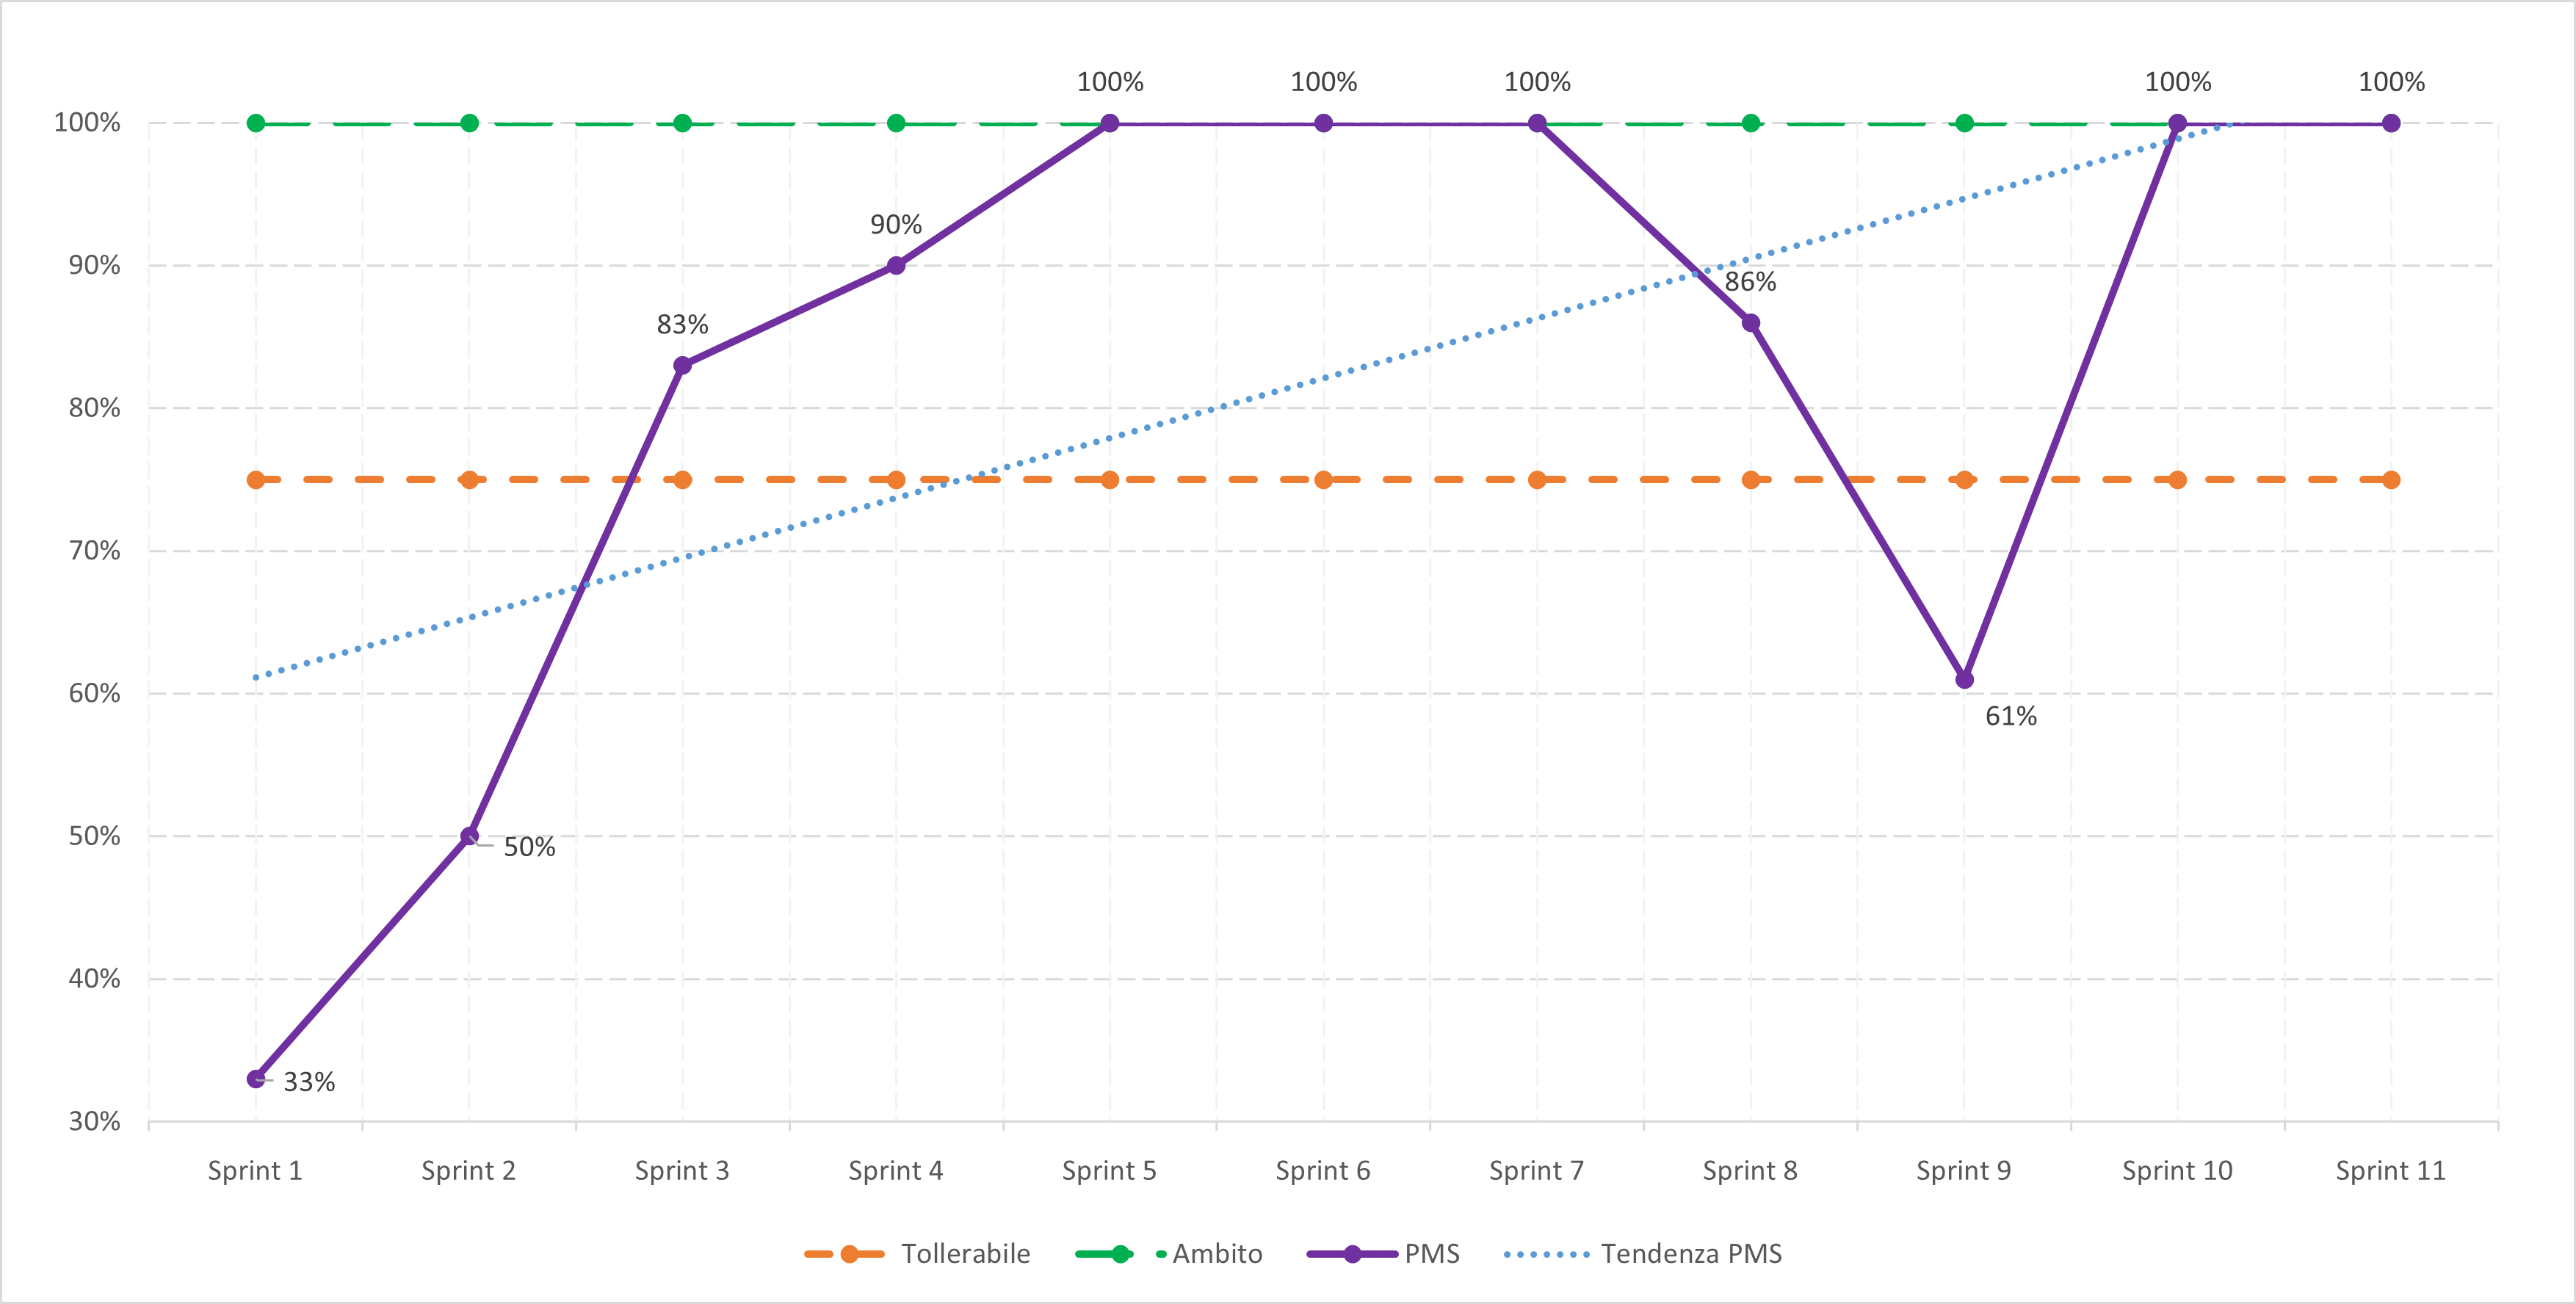
\includegraphics[width=15.5cm]{img/metriche/MPC1PMS.png}
\caption{M.PC.1.PMS - Percentuale di metriche soddisfatte.}
\end{figure}
\subsubsection{Considerazioni}
Osservando il grafico si nota come, per la maggior parte delle metriche, inizialmente non sia stata raggiunta la soglia tollerabile.
La difficoltà nel portare qualità al progetto era dovuta all’inesperienza iniziale, che ha portato il gruppo ad esplorare con cautela i vari aspetti del progetto.
Con il tempo, il team ha iniziato ad esporre più frequentemente le problematiche riscontrate, discutendo e proponendo migliorie.
Questo passo ha aiutato il gruppo a capire l’importanza della collaborazione e del dialogo aperto.
Alla fine del secondo sprint, il team ha iniziato a porre più attenzione al PDCA e alla definizione del proprio Way of working nelle Norme di progetto, aumentando notevolmente la qualità dei processi.
È possibile notare infatti un netto miglioramento a partire dal terzo sprint, fino ad arrivare ad un valore ambito, alla fine del quinto sprint. 
Il team punta a mantenere la stessa qualità anche per quanto riguarda le metriche di prodotto, le cui misurazioni verranno effettuate una volta iniziate le attività di progettazione, codifica e testing del processo di sviluppo.
\subsection{M.PC.2.RNP}
\begin{figure}[H]
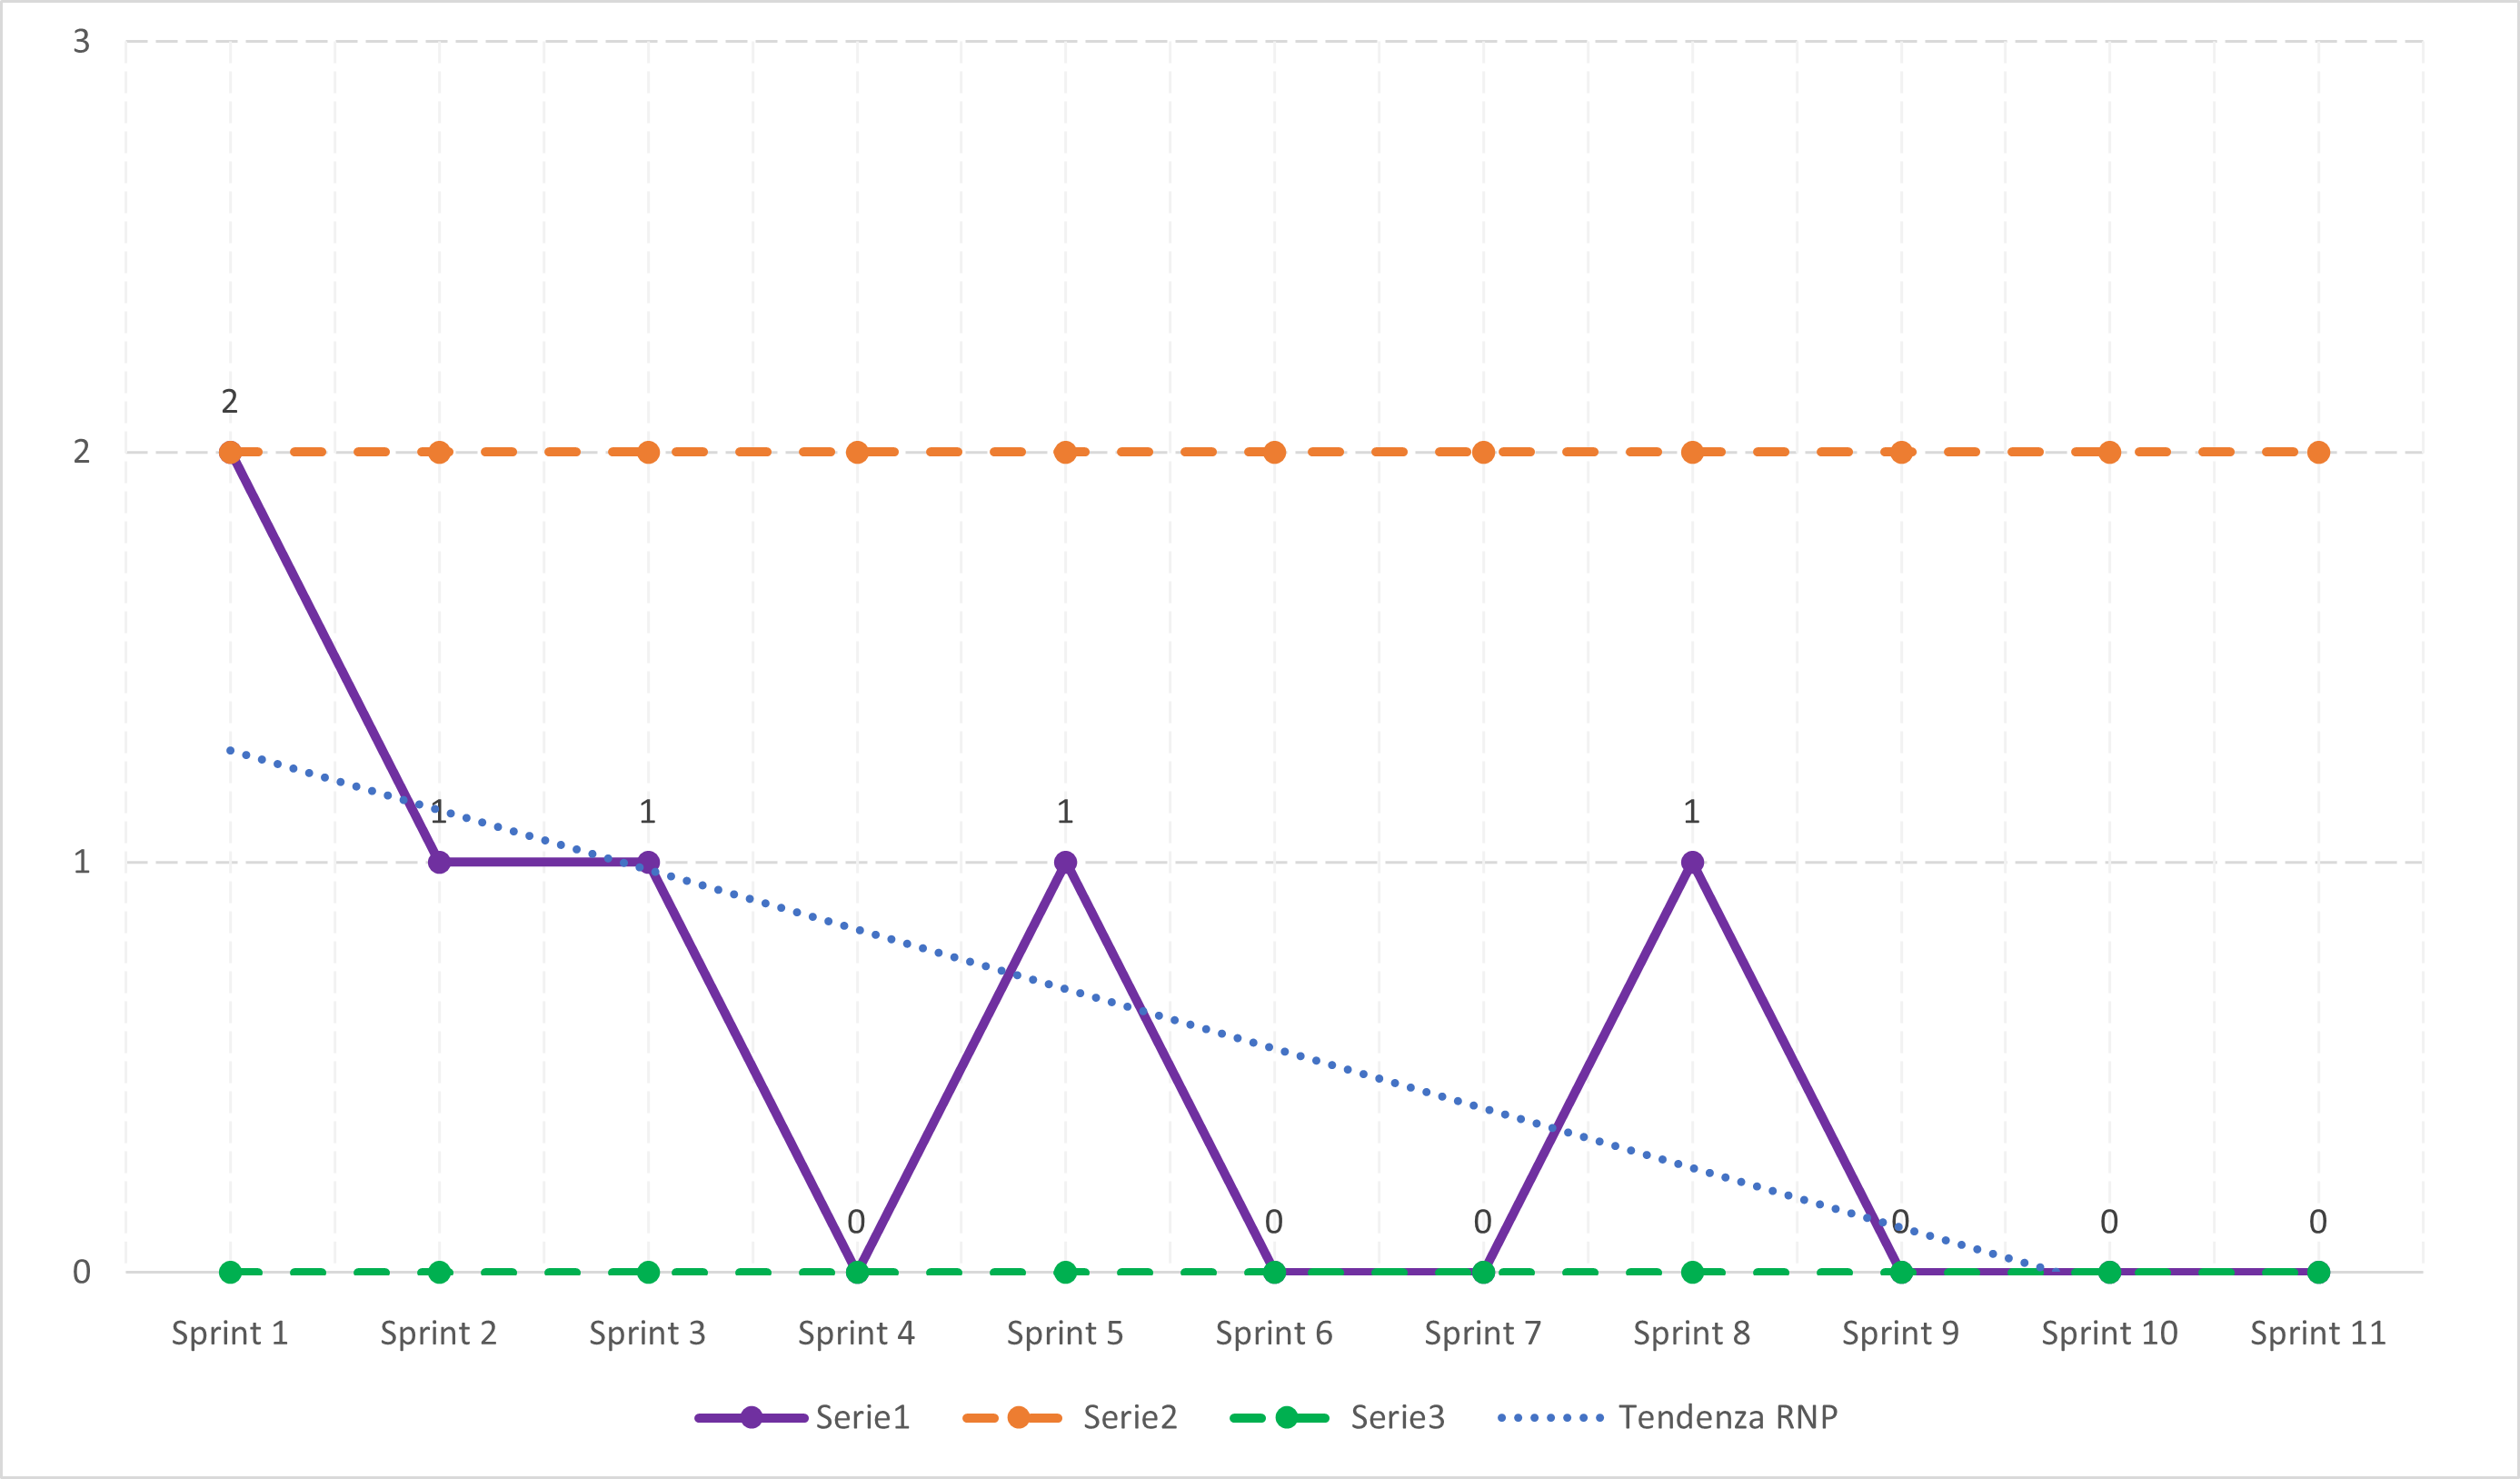
\includegraphics[width=15.5cm]{img/metriche/MPC2RNP.png}
\caption{M.PC.2.RNP - Rischi non previsti.}
\end{figure}
\subsubsection{Considerazioni}
Attraverso il grafico possiamo notare un'iniziale difficoltà nell'individuare i possibili rischi.
Si sono infatti presentati due imprevisti che sono emersi a causa della nostra inesperienza generale.
Tuttavia, il team è riuscito a mantenere la misurazione entro i limiti di tolleranza, gestendo i rischi pervenuti con metodo e ragionamento.
Nel quarto sprint non è stato riscontrato alcun rischio, raggiungendo così il livello desiderato.
Nel quinto sprint il team ha incontrato una nuova problematica legata alla scarsa comunicazione tra i membri, dovuta a impegni extra-universitari e periodi festivi.
In linea di massima, il team ha quindi inizialmente sottovalutato i rischi, imparando poi ad affrontarli in modo più professionale, riportandoli e tracciandoli in modo dettagliato attraverso discussioni documentate nei vari verbali.
\subsection{M.PC.3.VP}
\begin{figure}[H]
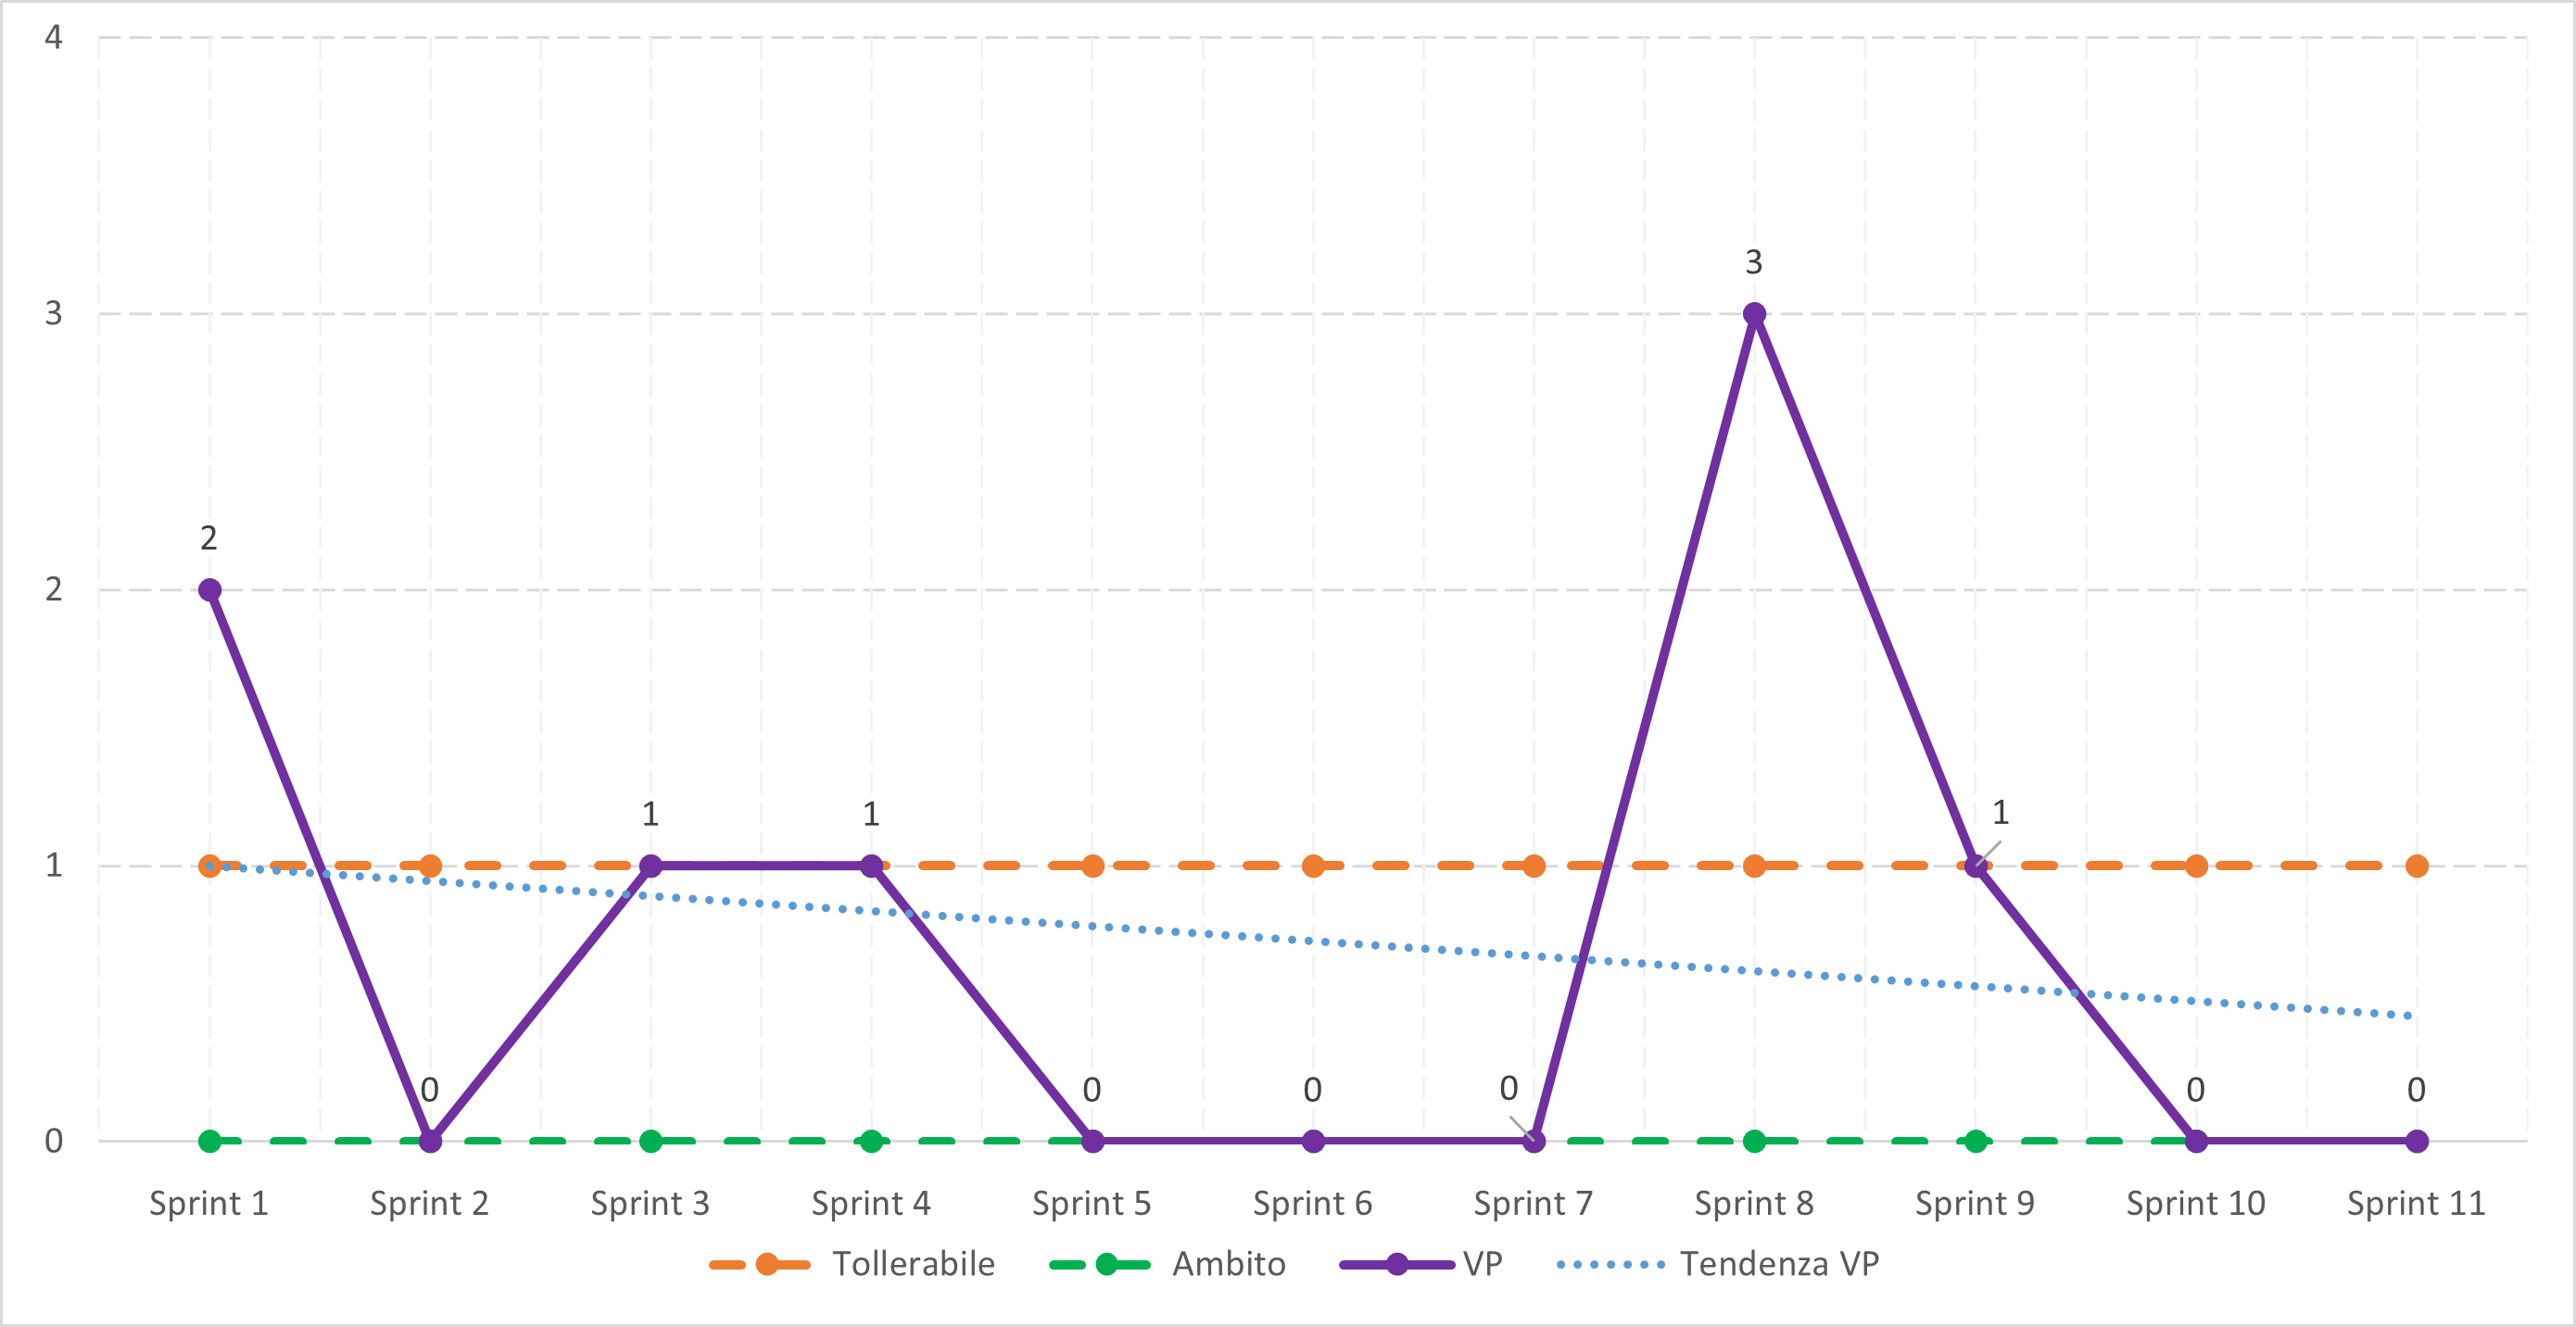
\includegraphics[width=15.5cm]{img/metriche/MPC3VP.png}
\caption{M.PC.3.VP - Variazione di piano.}
\end{figure}
\subsubsection{Considerazioni}
Inizialmente il team ha avuto difficoltà nel mantenere un ritmo adeguato e una pianificazione accurata.
A causa di una sovraccarico della quantità di lavoro assegnata ad ogni membro e di una pianificazione superficiale, si è verificata una discrepanza significativa tra i compiti pianificati e quelli effettivamente completati.
Tuttavia, nel secondo sprint, il team ha preso decisioni più precise e prudenti, raggiungendo un livello ottimale di performance.
Successivamente, dopo due sprint con un leggero technical debt legato alla grande quantità di lavoro pianificato, il team è riuscito a ristabilire il valore ambito durante il quinto e sesto sprint.
\subsection{M.PC.4.VC}
\begin{figure}[H]
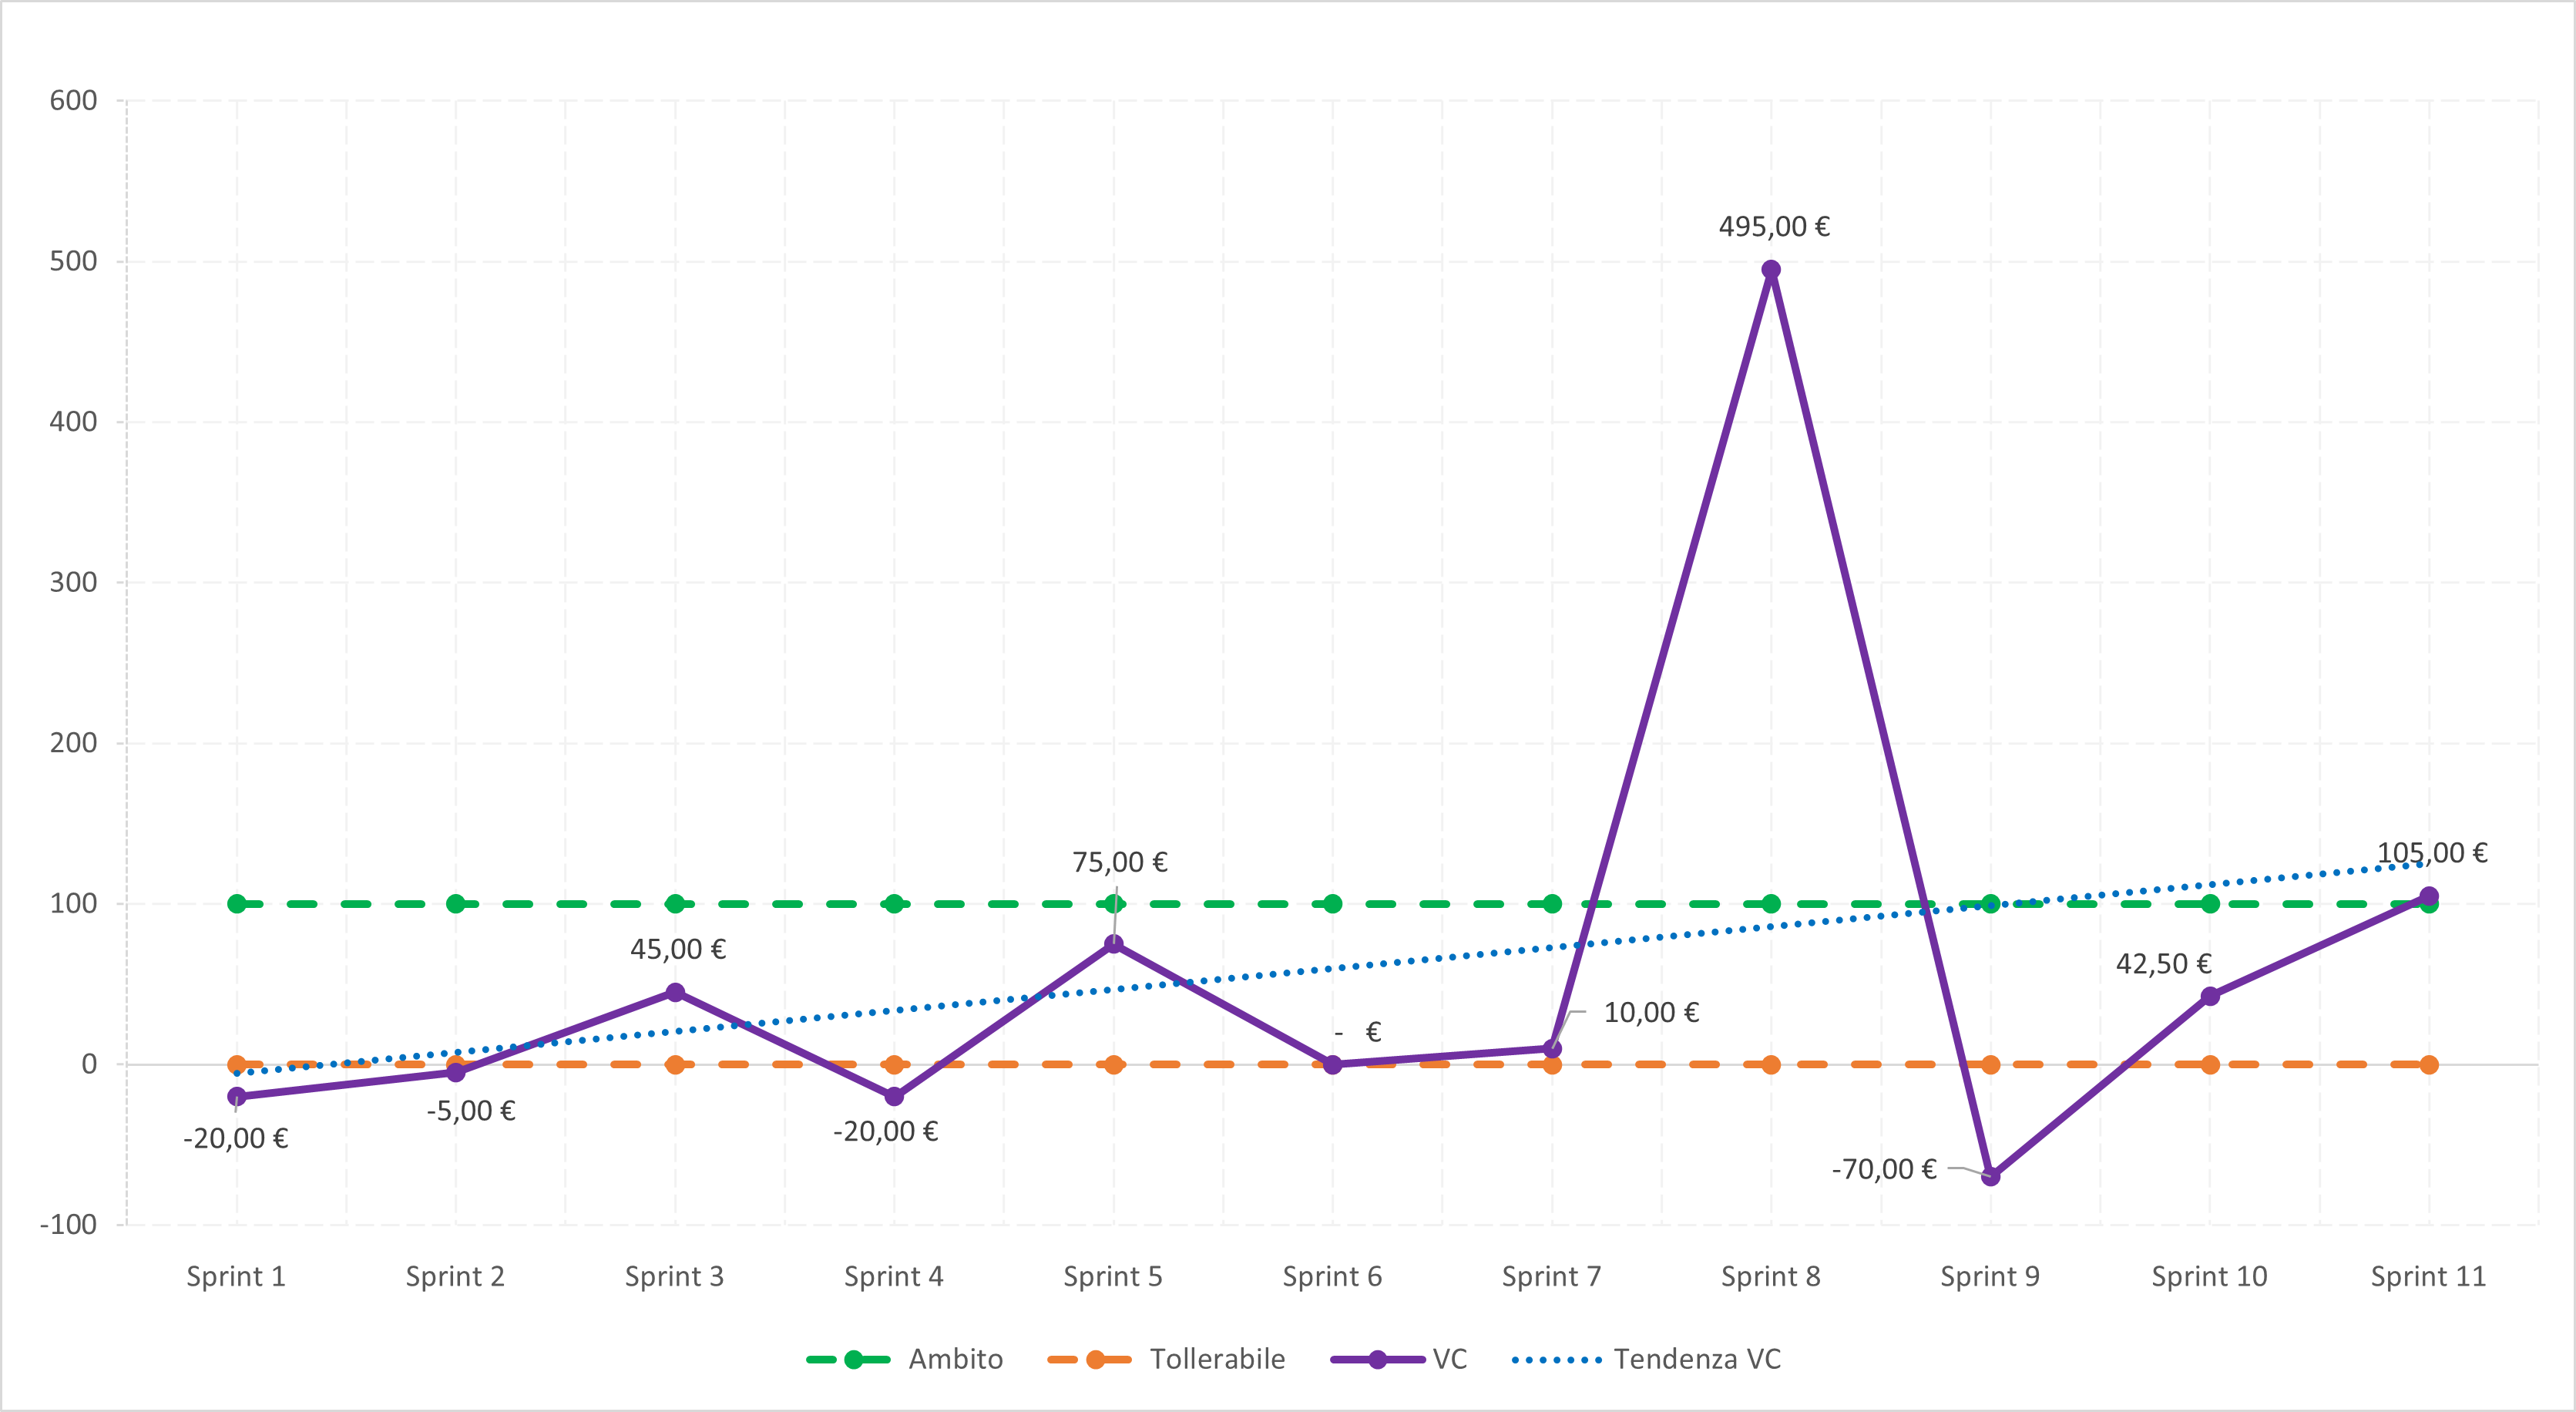
\includegraphics[width=15.5cm]{img/metriche/MPC4VC.png}
\caption{M.PC.4.VC - Variazione di costo.}
\end{figure}
\subsubsection{Considerazioni}
Inizialmente il team ha sottovalutato la quantità di lavoro necessario per completare le attività pianificate, superando i costi stimati.
Nel terzo periodo, data una sovrastima dei costi di realizzazione del PoC, il team è riuscito a contenere le spese e rientrare nelle stime iniziali.
Durante il quarto sprint, il colloquio con il professor Cardin ha richiesto una ristrutturazione dell'Analisi dei requisiti, causando un aumento delle ore dedicate alla preparazione della prima revisione RTB.
Nonostante questo impegno aggiuntivo e apparentemente dispendioso, il team è riuscito a portare a termine lo sprint limitando le perdite.
Il gruppo punta a migliorare la pianificazione, ponendo più attenzione alla definizione dei task e alla loro stima oraria, cercando di abbassare la varianza, molto evidente nel grafico. 
\subsection{M.PC.5.ISR}
\begin{figure}[H]
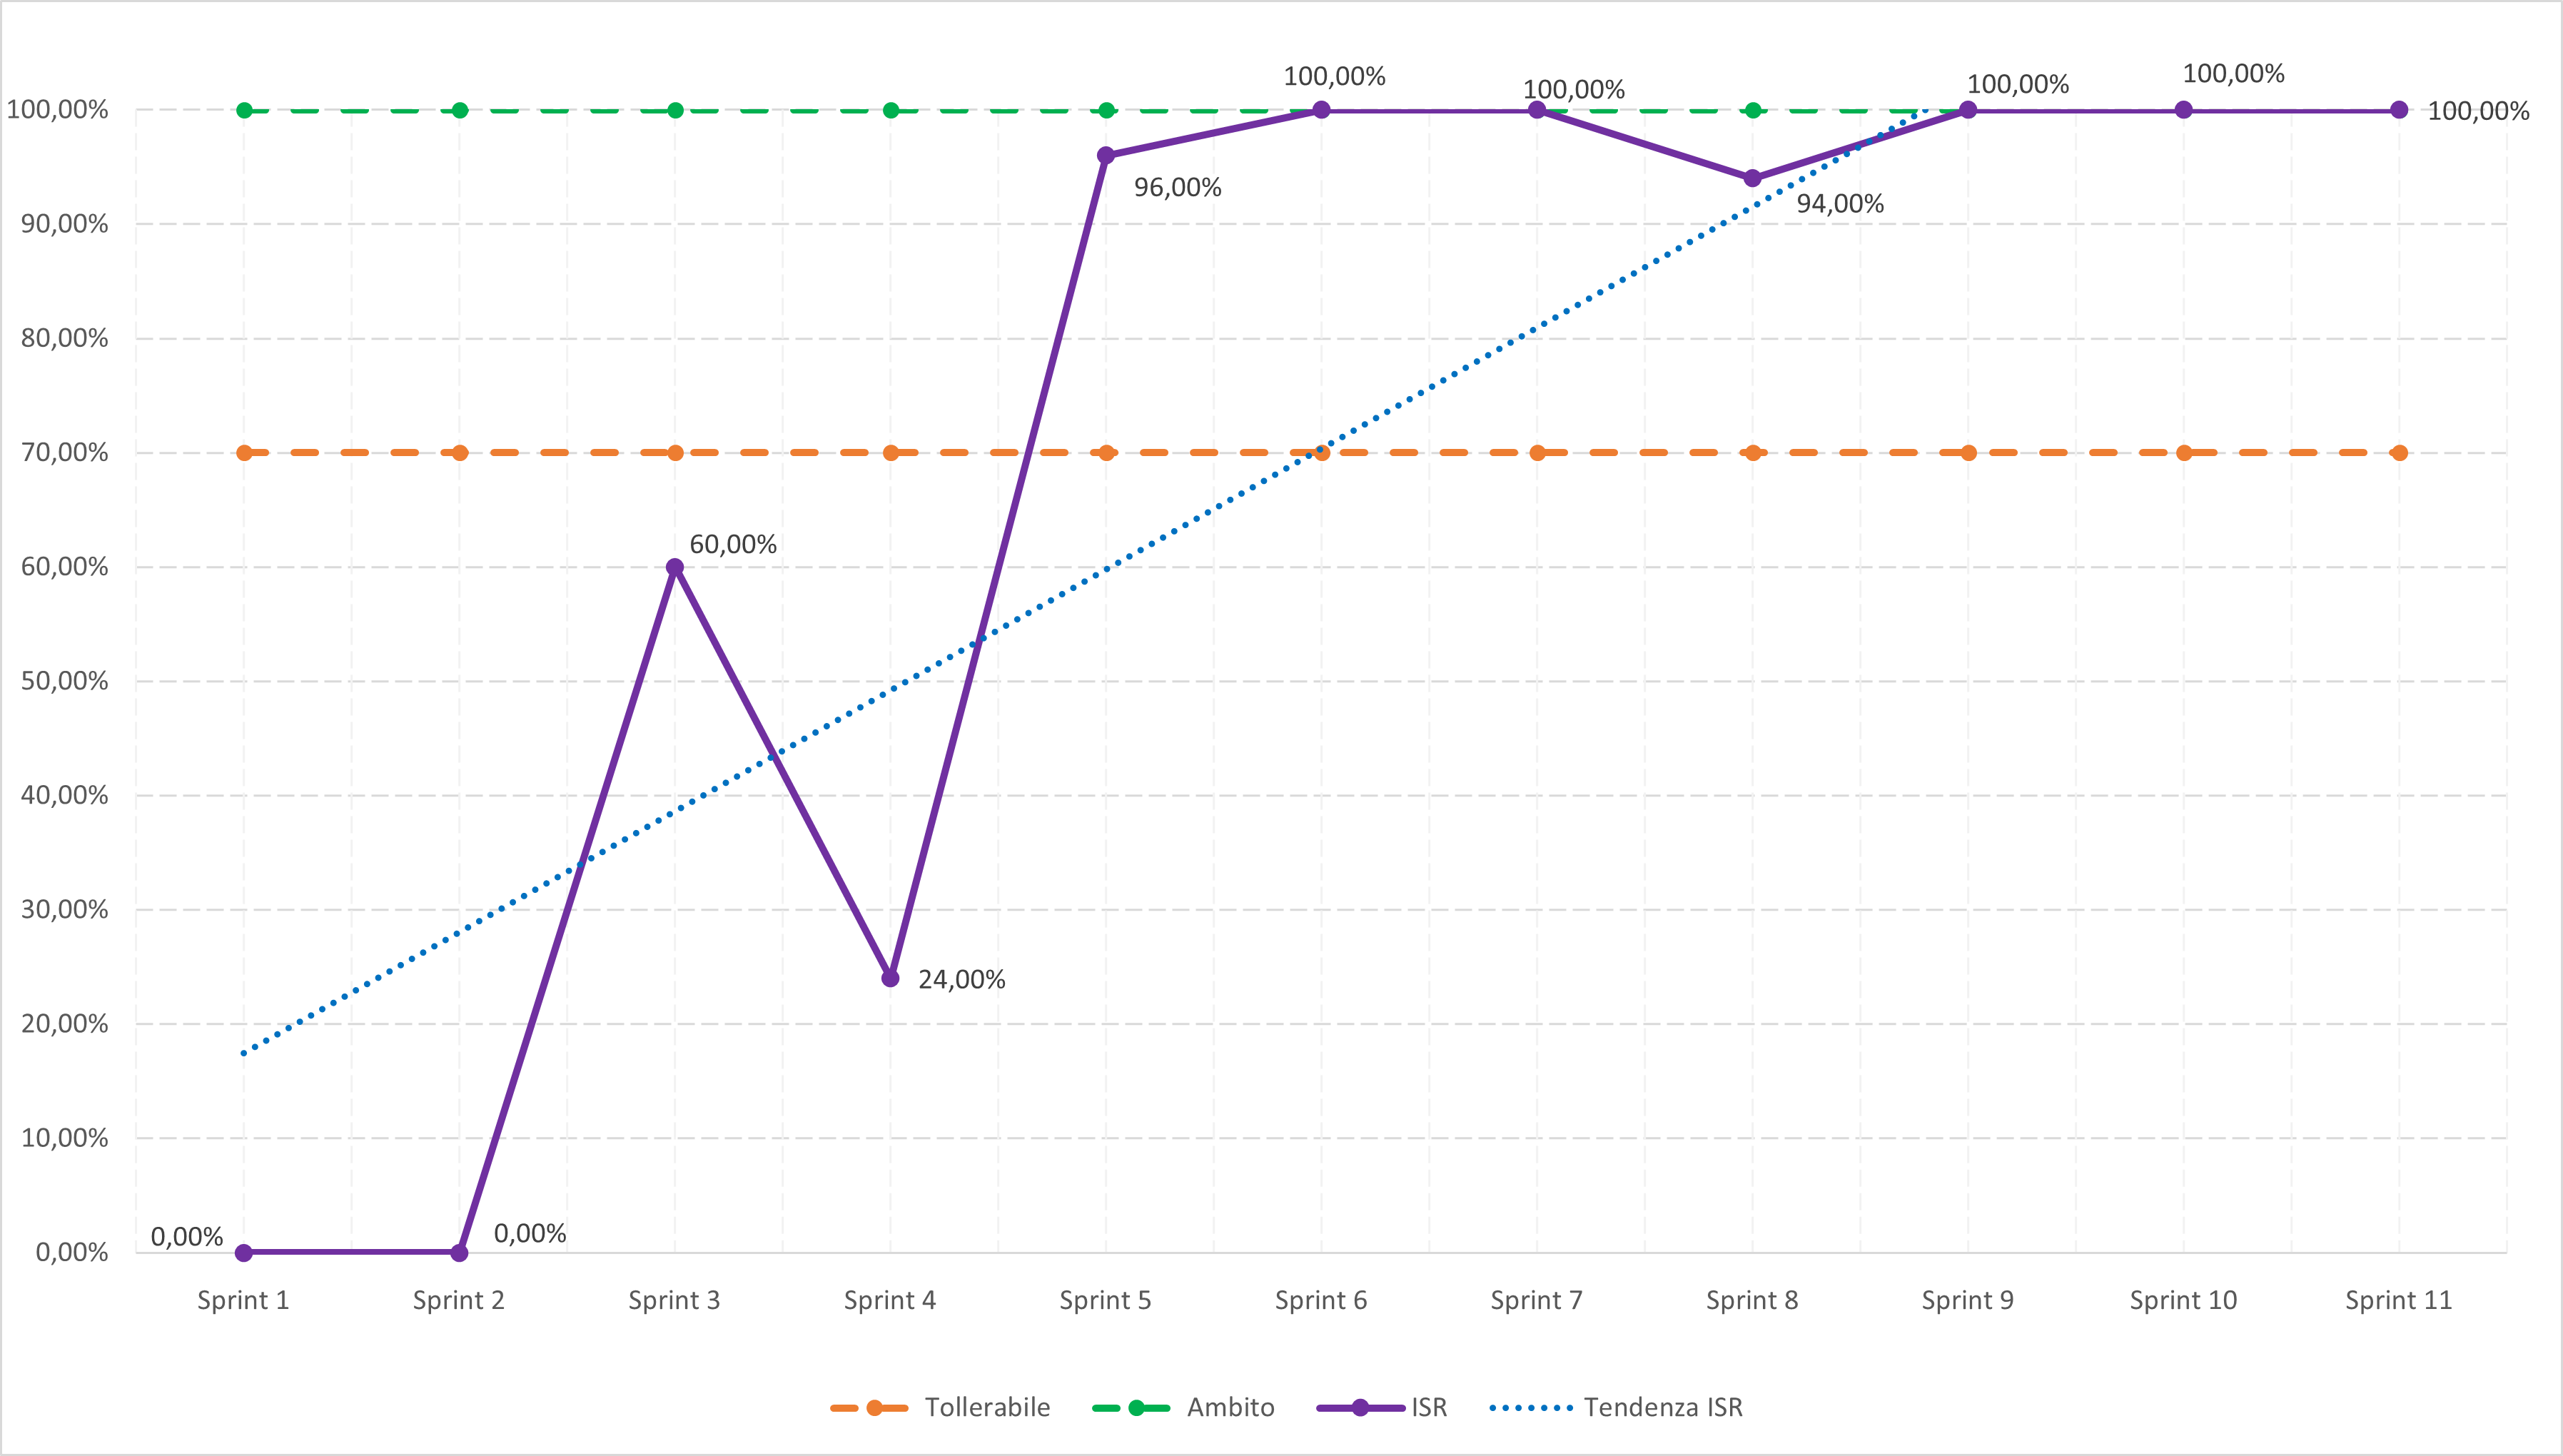
\includegraphics[width=15.5cm]{img/metriche/MPC5ISR.png}
\caption{M.PC.5.ISR - Indice di stabilità dei requisiti.}
\end{figure}
\subsubsection{Considerazioni}
Nei primi due sprint, la nostra inesperienza nella definizione di un gran numero di requisiti ha portato ad un'alta instabilità dei requisiti.
Nel terzo sprint, il team ha aggiunto numerosi requisiti, anche grazie a incontri interni ed esterni che hanno contribuito a rendere più chiare le funzionalità del prodotto.
Nel quarto sprint, dopo un incontro con il Professore Cardin, è stato necessario ristrutturare l'Analisi dei requisiti, sia per struttura del documento che per contenuto.
Nel quinto e sesto sprint, il team ha rapidamente ristabilito l'ordine, definendo un elenco dei requisiti che, al netto di eventuali modifiche future limitate, rappresenterà l'insieme finale che verrà considerato nello sviluppo dell'MVP.
\subsection{M.PC.6.CCM}
Questa metrica verrà misurata solo dopo il superamento della revisione RTB.
\subsection{M.PC.7.SC}
Questa metrica verrà misurata solo dopo il superamento della revisione RTB.
\subsection{M.PC.8.BC}
Questa metrica verrà misurata solo dopo il superamento della revisione RTB.
\subsection{M.PC.9.ET}
\begin{figure}[H]
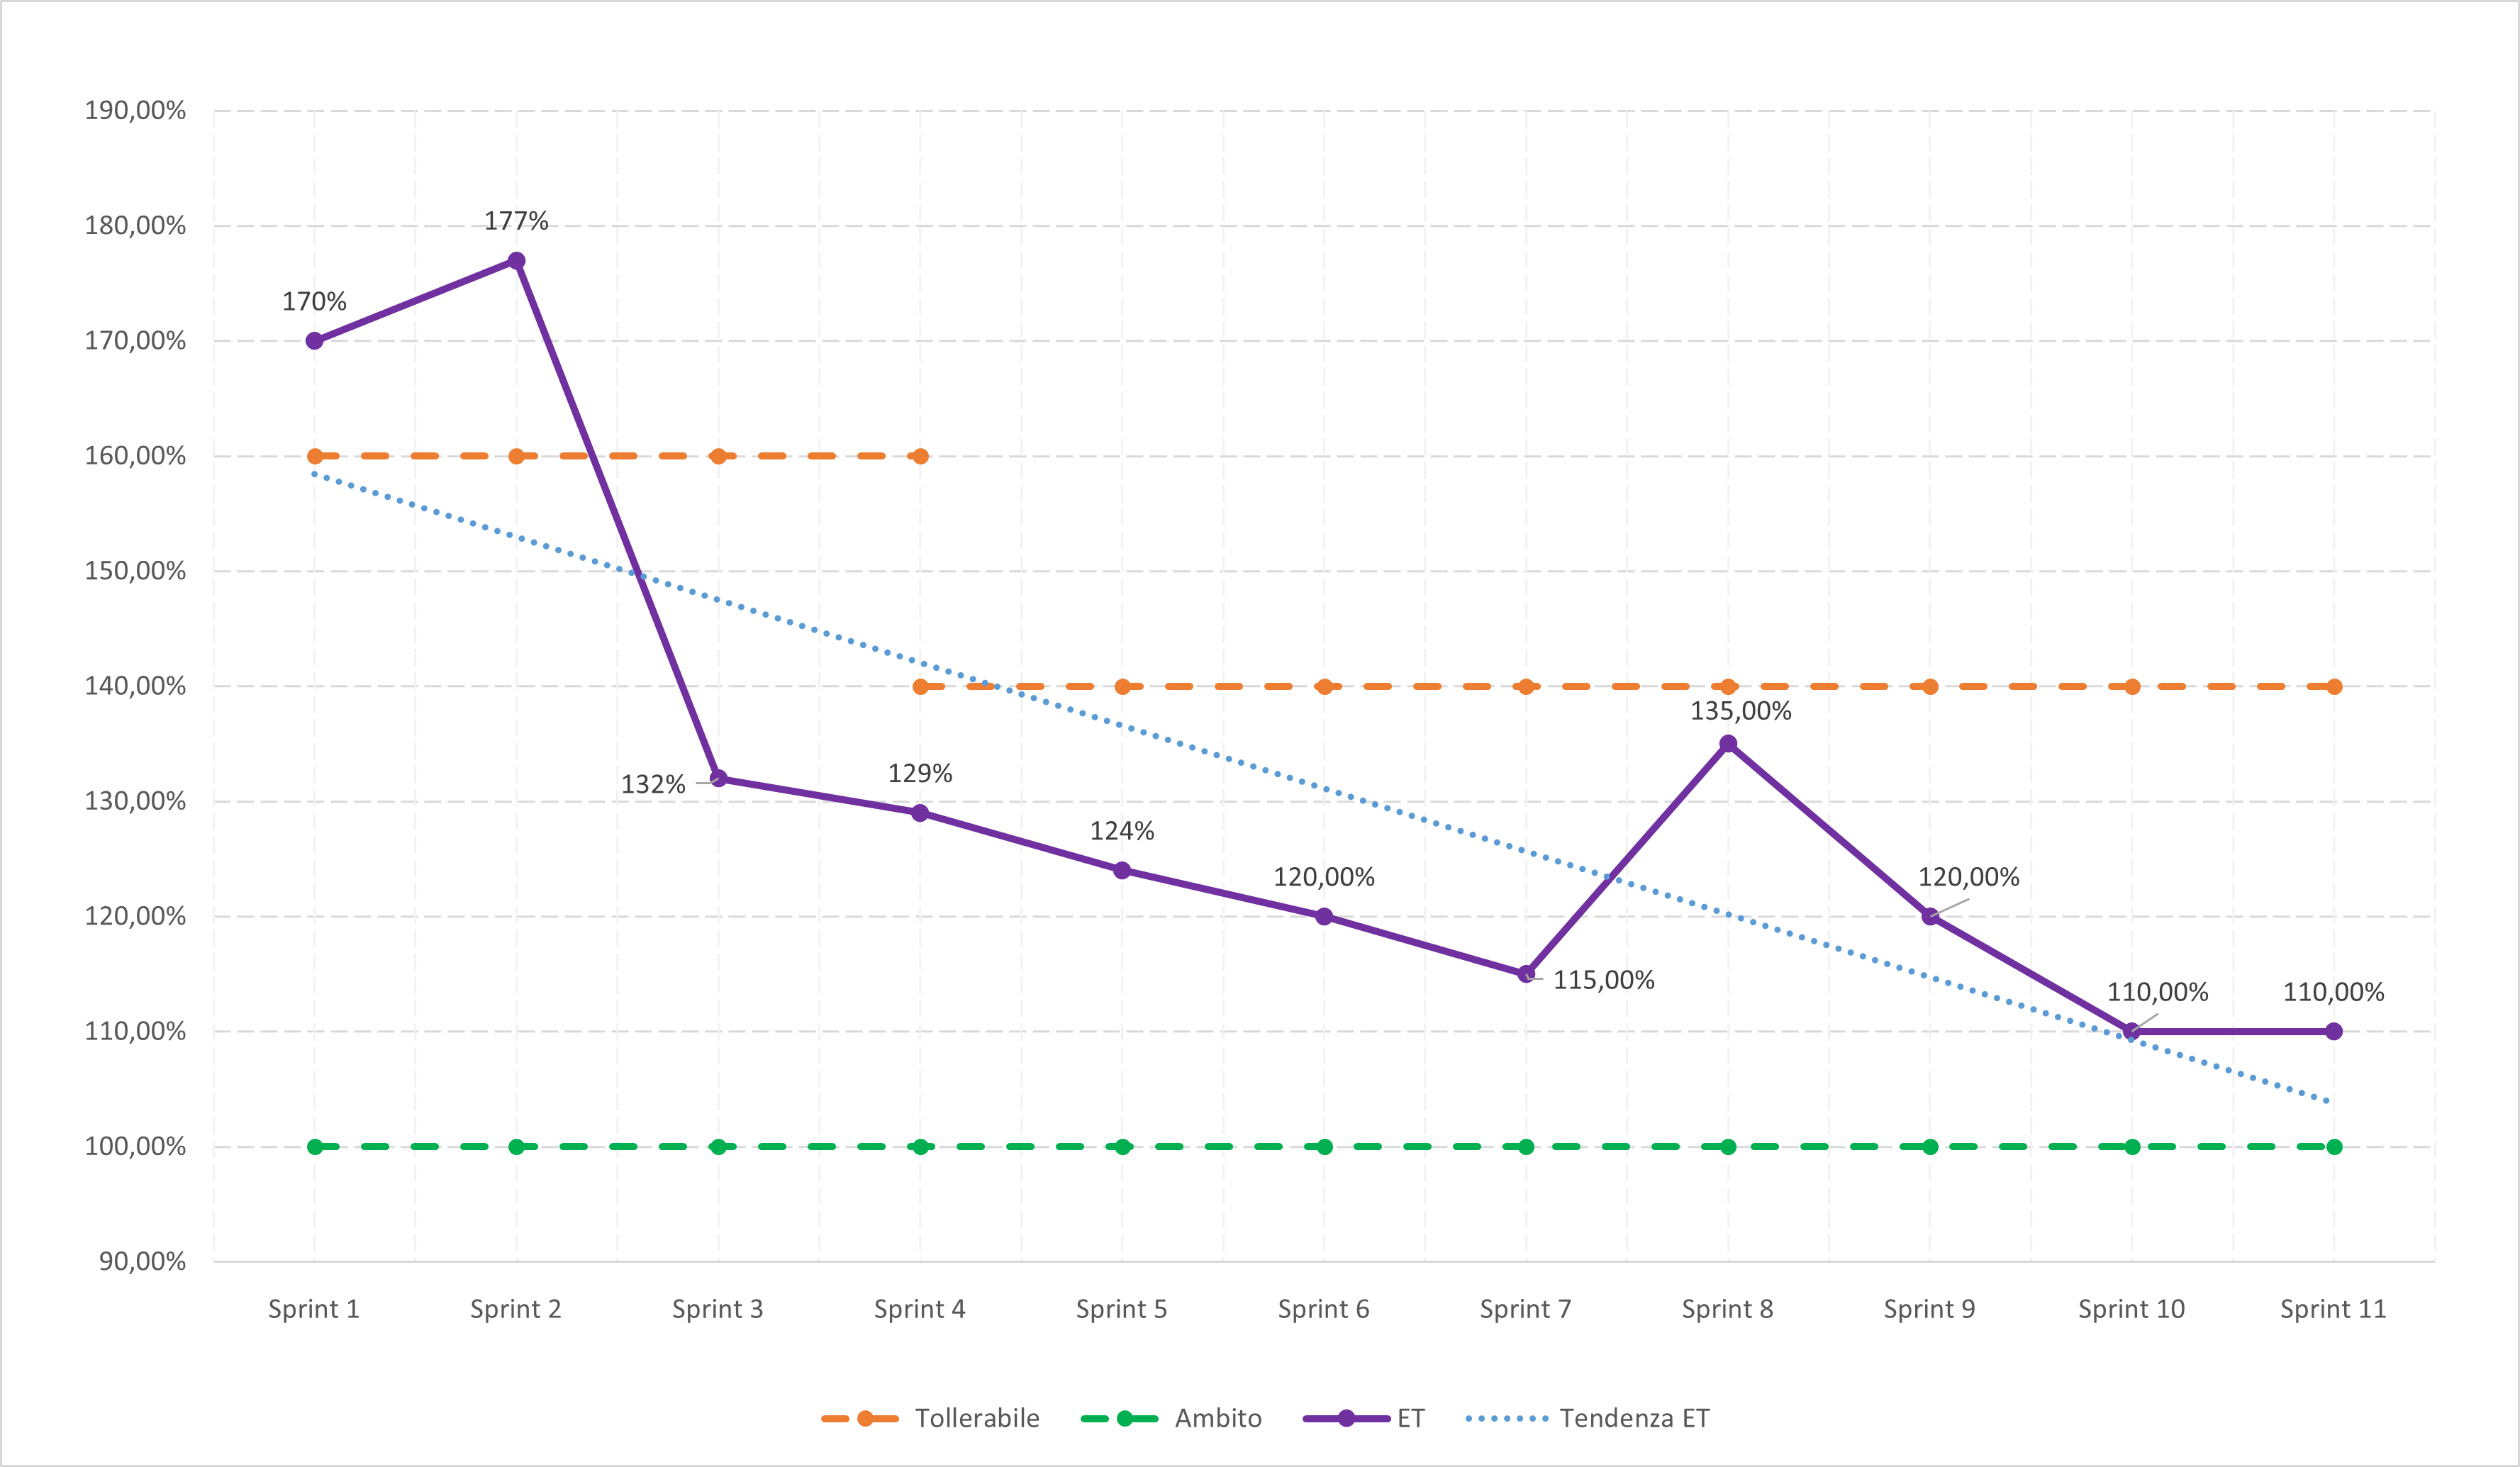
\includegraphics[width=15.5cm]{img/metriche/MPC9ET.png}
\caption{M.PC.9.ET - Efficienza temporale.}
\end{figure}
\subsubsection{Considerazioni}
Nonostante un inizio caratterizzato da un elevato rapporto tra ore di lavoro e ore produttive, dovuto all'inesperienza e alla scarsa familiarità con gli strumenti utilizzati, si è registrato un notevole miglioramento dal terzo sprint in poi.
Questo è stato possibile grazie al miglioramento delle norme, che hanno infatti ricoperto la funzione di guida durante lo svolgimento delle attività da parte dei componenti del gruppo.
Con l'obiettivo di migliorare in modo costante la qualità, il team ha deciso di ridurre la soglia tollerabile da 160\% a 140\%.
Il team punta a migliorare ulteriormente questo rapporto, ritenendolo uno degli indicatori più importanti da considerare nella valutazione dell'automiglioramento.
\subsection{M.PD.1.IG}
\begin{figure}[H]
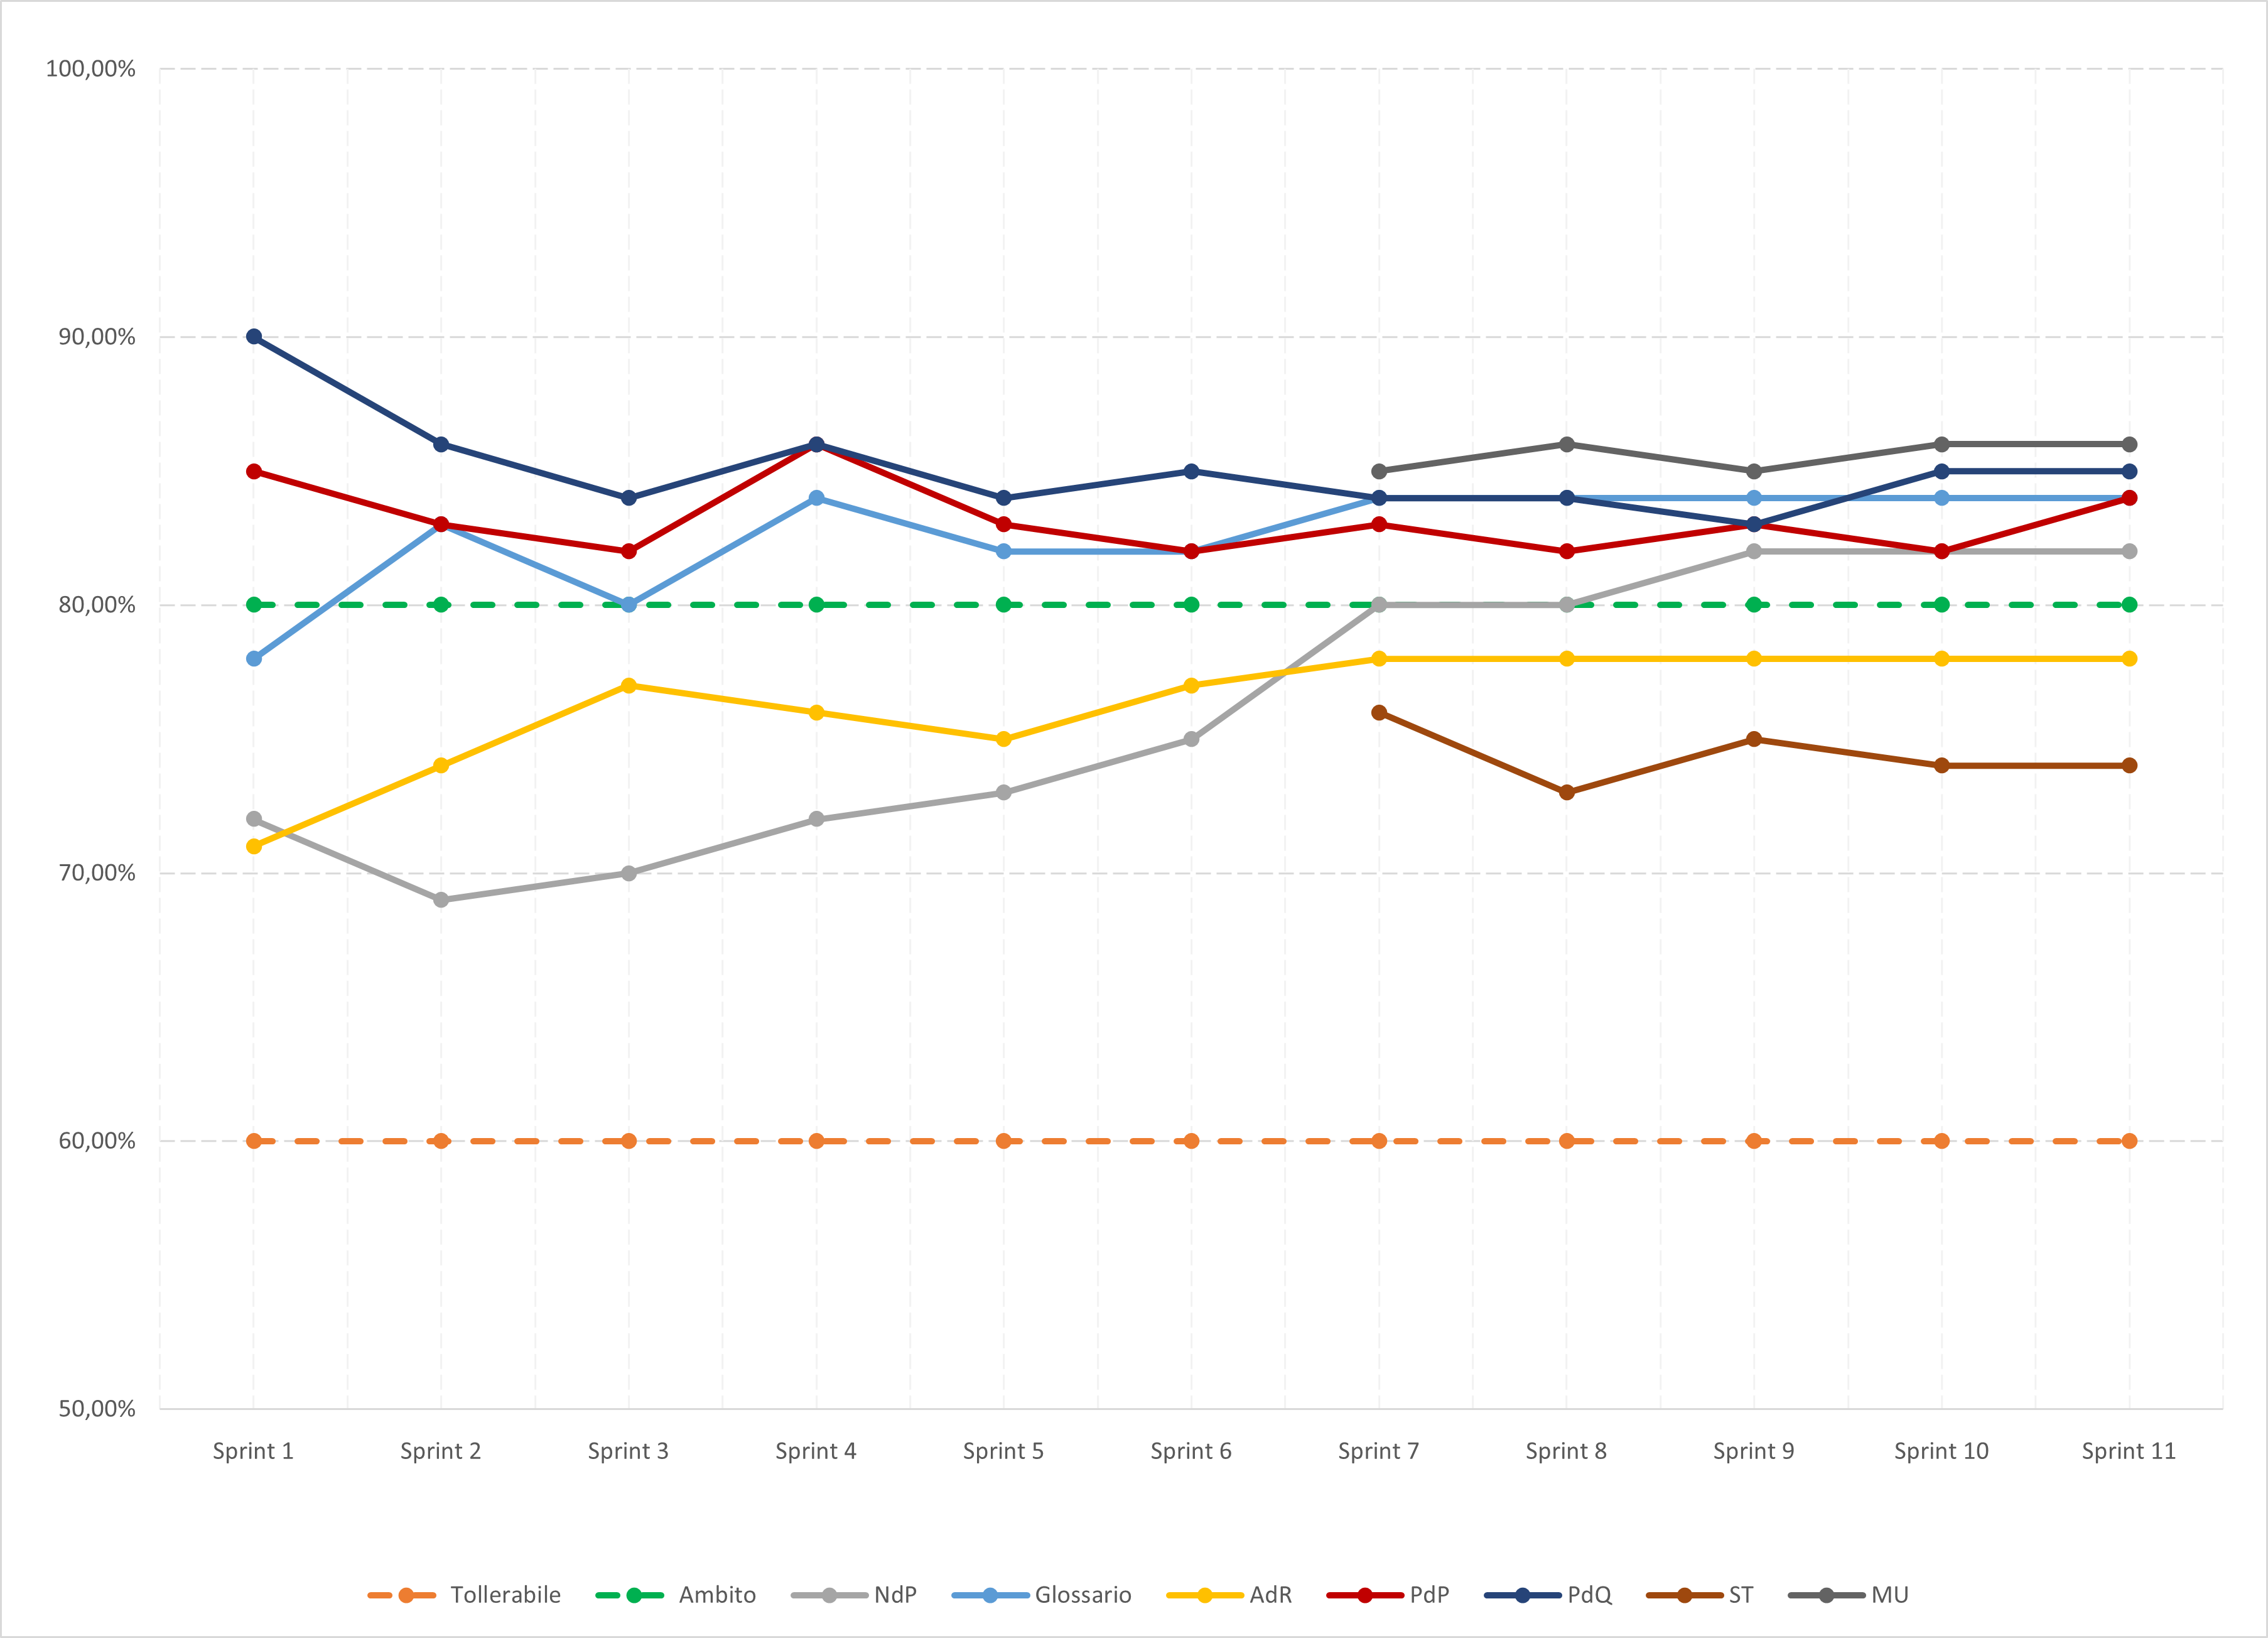
\includegraphics[width=15.5cm]{img/metriche/MPD1IG.png}
\caption{M.PD.1.IG - Indice di Gulpease.}
\end{figure}
\subsubsection{Considerazioni}
Tutti i documenti sono facilmente comprensibili anche per chi ha una licenza media, poiché rispettano la soglia di tolleranza del 60\%.
Trattando argomenti più specifici, le Norme di progetto utilizzano frasi più elaborate, rendendo l'indice di leggibilità di tale documento leggermente più basso degli altri.
Il gruppo pensa di continuare a migliorare questo indice rielaborando i periodi lunghi, abbreviandoli o riformulando i concetti esposti ove possibile.
\subsection{M.PD.2.LMC}
Questa metrica verrà misurata solo dopo il superamento della revisione RTB.
\subsection{M.PD.3.AFS}
Questa metrica verrà misurata solo dopo il superamento della revisione RTB.
\subsection{M.PD.4.AR}
Questa metrica verrà misurata solo dopo il superamento della revisione RTB.
\subsection{M.PD.5.RD}
Questa metrica verrà misurata solo dopo il superamento della revisione RTB.
\subsection{M.PD.6.LCG}
Questa metrica verrà misurata solo dopo il superamento della revisione RTB.
\subsection{M.PD.7.CD}
Questa metrica verrà misurata solo dopo il superamento della revisione RTB.
\subsection{M.PD.8.IM}
Questa metrica verrà misurata solo dopo il superamento della revisione RTB.
\subsection{M.PD.9.TS}
Questa metrica verrà misurata solo dopo il superamento della revisione RTB.
\subsection{M.PD.10.CSD}
Questa metrica verrà misurata solo dopo il superamento della revisione RTB.
\subsection{M.PD.11.AFPH}
Questa metrica verrà misurata solo dopo il superamento della revisione RTB.
\subsection{M.PD.12.TR}
Questa metrica verrà misurata solo dopo il superamento della revisione RTB.
\subsection{M.PD.13.EI}
Questa metrica verrà misurata solo dopo il superamento della revisione RTB.

\end{document}